\documentclass[12pt, a4paper]{article}
\pagestyle{plain}
\setlength{\parindent}{0in}
\setlength{\parskip}{2mm}

\usepackage{geometry}
% \geometry{bindingoffset=4cm}
\geometry{bindingoffset=0cm}

%%%%%%%%%%%%%%%%%%%%%%%%%%%%%
% PACKAGES & ENVIRONMENTS
%%%%%%%%%%%%%%%%%%%%%%%%%%%%%

% \usepackage[margin=0.75in]{geometry}   % Put this in each specific document to choose margin

\usepackage{amssymb,amsmath,amsthm}
\usepackage{makeidx}
%\usepackage{MnSymbol}
\usepackage{latexsym}
\usepackage{enumerate}
\usepackage{hyperref}		%% For URLs
% \usepackage{calrfsf}		%% For scroll font \mathscr{}
%\usepackage{todonotes}		%% For \todo{} margin notes
\usepackage{tikz}

\theoremstyle{definition}  %% Use non-italic text for body of Theorem


\newtheorem{Definition}{Definition}
\newtheorem{Corollary}{Theorem}
\newtheorem{Theorem}{Theorem}
\newtheorem*{Proof}{Proof}
\newtheorem{Lemma}{Lemma}
\newtheorem{Example}{Example}


% \usepackage{delarray}

%\usepackage[all,cmtip,2cell]{xy}
%\UseAllTwocells
%\input xy
%\xyoption{all}
%\xyoption{v2}

%%%%%%%%%%%%%%%%%%%%%%%%%%%%%
% STANDARD NEW COMMANDS
%%%%%%%%%%%%%%%%%%%%%%%%%%%%%

\newcommand{\upwedge}{\wedge}
\newcommand{\downwedge}{\vee}
\newcommand{\glb}{\wedge}
\newcommand{\lub}{\vee}


\newcommand{\tstile}{\vdash}
\newcommand{\makestrue}{\models}

\newcommand{\andalso}{,\;}		%% Comma with more space, for premises


% \newcommand{\newIdea}[1]{\emph{#1}} %% Emphasis for the first intro of new terminology
\newcommand{\newIdea}[1]{\textbf{#1}} %% Bold text for the first intro of new terminology
\newcommand{\terminology}[1]{\textbf{#1}} %% Bold text for the first intro of new terminology
\newcommand{\pr}[1]{\ensuremath{{#1}^{\prime}}}

\newcommand{\cat}[1]{\ensuremath{\mathcal{#1}}}
\newcommand{\category}[1]{\ensuremath{\mathcal{#1}}}
\newcommand{\Sets}{{\textsc{Sets}}}

\newcommand{\following}{\circ}

\renewcommand{\emptyset}{\varnothing}  %% Use the nice symbol
% \newcommand{\Hom}[1]{\ensuremath{\mbox{\textup{Hom}}_{#1}}}
% \newcommand{\Nat}{\mbox{\textup{Nat}}}
\newcommand{\Id}[1]{\ensuremath{\mbox{\textup{Id}}_{#1}}}
\newcommand{\monoidunit}[1]{\ensuremath{\mathbf{1}_{#1}}}
% \newcommand{\nt}{natural transformation}
% \newcommand{\NT}{Natural transformation}

%% Numbers:
\newcommand{\CC}{\ensuremath{\mathbb{C}}} %% Complex numbers
\newcommand{\RR}{\ensuremath{\mathbb{R}}} %% Real numbers
\newcommand{\QQ}{\ensuremath{\mathbb{Q}}} %% Rational numbers
\newcommand{\NN}{\ensuremath{\mathbb{N}}} %% Natural numbers
\newcommand{\ZZ}{\ensuremath{\mathbb{Z}}} %% Integers
\newcommand{\BB}{\ensuremath{\mathbb{B}}} %% Booleans

\newcommand{\HomSet}[2]{\ensuremath{\{{#1} \to {#2}\}}}

%% Logical notation:
\newcommand{\AND}{\,\&\,}
\newcommand{\OR}{\vee}
\newcommand{\NOT}{\neg}
\newcommand{\IMPLIES}{\Rightarrow}
\newcommand{\ABSURDITY}{\bot}
\newcommand{\intersect}{\cap}
\newcommand{\union}{\cup}
\newcommand{\iso}{\cong}

\newcommand{\set}[1]{\ensuremath{
\{ #1 \}
}}  %% Curly brackets for sets
\newcommand{\setSuchThat}[2]{\ensuremath{
\{ #1 \,|\, #2 \}
}}  %% Curly brackets with 'pipe' divider for sets with conditions


\newcommand{\List}[1]{\texttt{List(}#1\texttt{)}}
%\newcommand{\List}[1]{\texttt{[}#1\texttt{]}}
\newcommand{\Nil}{\texttt{[\;]}}
\newcommand{\ListOf}[2]{
\texttt{[}
#1
\texttt{||}
#2
\texttt{]}
}

\newcommand{\BTree}[1]{\texttt{BTree(}#1\texttt{)}}



% %% Some type-theory notation
\newcommand{\mono}[1]{\texttt{#1}}
% \newcommand{\term}[1]{\texttt{\ensuremath{#1}}}
\newcommand{\term}[1]{\texttt{#1}}
% \newcommand{\type}[1]{\texttt{\ensuremath{#1}}}
\newcommand{\type}[1]{\texttt{#1}}

\newcommand{\DefinedAs}{:\equiv}

%\newcommand{\TermOfType}[2]{\term{#1}:\type{#2}}
%\newcommand{\ToT}[2]{\term{#1}:\type{#2}}		%% ToT = TermOfType

%\newcommand{\IdMathrm}{\mathrm{Id}}
\newcommand{\Identity}[2]{#1 \! = \! #2}
\newcommand{\IdType}[3]{#1 \! =_{#3}\! #2}
\newcommand{\ii}{\iota}
\newcommand{\pind}[1]{\texttt{pind}_{#1}}

\newcommand{\s}{\term{s}}					% successor in \NN
\newcommand{\zN}{\term{0}_{\type{\NN}}}		% zero of \NN
\newcommand{\N}[1]{\term{#1}_{\type{\NN}}}  % numerals of \NN

\newcommand{\fin}[2]{\term{#1}_{\term{#2}}}


\newcommand{\JEqTerms}[3]{\ensuremath{\term{#1} \!\equiv\! \term{#2}:\type{#3} }}
\newcommand{\JEqTypes}[2]{\ensuremath{\type{#1} \!\equiv\! \type{#2}}}

\newcommand{\ctx}{\,\textrm{ctx}}

\newcommand{\PROD}[2]{\ensuremath{\prod_{#1} #2}}
\newcommand{\SUM}[2]{\ensuremath{\sum_{#1} #2}}
\newcommand{\AltPROD}[2]{\ensuremath{\langle{#1}\rangle \to #2}}
\newcommand{\AltSUM}[2]{\ensuremath{\langle{#1}\rangle \x #2}}
\newcommand{\TYPE}{\type{TYPE}}

%\newcommand{\PType}[2]{\type{#1}\,\ensuremath{\times}\,\type{#2}}
%\newcommand{\CType}[2]{\type{#1}\,\ensuremath{+}\,\type{#2}}
%\newcommand{\FType}[2]{\type{#1}\,\ensuremath{\to}\,\type{#2}}

\newcommand{\x}{\times}
\newcommand{\+}{+}
\newcommand{\z}{\type{0}}

\newcommand{\rec}[1]{\ensuremath{\texttt{rec}_{#1}}}
\newcommand{\ind}[1]{\ensuremath{\texttt{ind}_{#1}}}


\newcommand{\inl}{\texttt{inl}}
\newcommand{\inr}{\texttt{inr}}

\newcommand{\refl}[1]{\ensuremath{\textrm{refl}_{#1}}}

%%%%%%%%%%%%%%%%%%%%%%%%%%%%%
% DIAGRAM TEMPLATES
%%%%%%%%%%%%%%%%%%%%%%%%%%%%%

% A shortcut to make commutative squares: single-spaced
\newcommand{\SmallCommutativeSquare}[8]{
% Usage: \SmallCommutativeSquare{Top Left Object}{Top Right Object}{Bottom Left Object}{Bottom Right Object}{Top Arrow}{Left Arrow}{Right Arrow}{Bottom Arrow}
\xymatrix{
{#1} \ar[r]^{{#5}} \ar[d]_{{#6}} & {#2}\ar[d]^{{#7}} \\
{#3} \ar[r]_{{#8}}& {#4}
}
}

% A shortcut to make commutative squares: double-spaced
\newcommand{\LargeCommutativeSquare}[8]{
% Usage: \LargeCommutativeSquare{Top Left Object}{Top Right Object}{Bottom Left Object}{Bottom Right Object}{Top Arrow}{Left Arrow}{Right Arrow}{Bottom Arrow}
\xymatrix{
{#1} \ar[rr]^{{#5}} \ar[dd]_{{#6}} && {#2}\ar[dd]^{{#7}} \\
\\
{#3} \ar[rr]_{{#8}}&& {#4}
}
}


% A shortcut to make ``tent diagrams'' for natural transformations
\newcommand{\NatTransDiag}[9]{
% Usage: \NatTransDiag{Object 1}{Object 2}{Arrow}{Functor 1}{Functor 2}{Category 1}{Category 2}{NT Name}{Curvature of arrows}
\xymatrix{
&{#1} \ar[rrr]^{{#3}} \ar@/^{#9}/[ddddr]^{{#5}} \ar@/_{#9}/[dddl]_{{#4}} &&&{#2}\ar@/^{#9}/[ddddr]^{{#5}}\ar@/_{#9}/[dddl]_{{#4}}  &&& {#6} \ar@{-->}[dddd]^{{#4},\, {#5}}\\
\\
\\
{#4}({#1})\ar[drr]^{{#8}_{#1}} \ar@{->}[rrr]^{{#4}({#3})}	&&&	{#4}({#2})\ar[drr]^{{#8}_{#2}}  \\
&&	{#5}({#1})\ar[rrr]_{{#5}({#3})} 	&&&	{#5}({#2}) && {#7}
}}



% A shortcut to make ``constraint diagrams'' for natural transformations
\newcommand{\NTConstraint}[6]{
% Usage: \NTConstraint{NT Name}{Functor 1}{Functor 2}{Object 1}{Object 2}{Arrow}
\LargeCommutativeSquare
{{#2}({#4})}	% Top Left Object
{{#2}({#5})}	% Top Right Object
{{#3}({#4})}	% Bottom Left Object
{{#3}({#5})}	% Bottom Right Object
{{#2}({#6})}	% Top Arrow
{{#1}_{#4}}		% Left Arrow
{{#1}_{#5}}		% Right Arrow
{{#3}({#6})}	% Bottom Arrow
}




%%%%%%%%%%%%%%%%%%%%%%%%%%%%%
% Putting date \& time, section number into header of every page
%%%%%%%%%%%%%%%%%%%%%%%%%%%%%
\usepackage{fancyhdr, datetime}
\setlength{\headheight}{15.2pt}
\renewcommand{\headrulewidth}{0.25pt}
\renewcommand{\footrulewidth}{0pt}
\pagestyle{fancy}
\fancyhf{}
\lhead{DRAFT: \currenttime, \today }
\rhead{Section \thesubsection}
\cfoot{\thepage}
%%%%%%%%%%%%%%%%%%%%%%%%%%%%%




%%%%%%%%%%%%%%%%%%%%%%%%%%%%%
\author{Stuart Presnell \& James Ladyman
\\stuart.presnell@bristol.ac.uk
\\james.ladyman@bristol.ac.uk
}
\title{A Primer on \\Homotopy Type Theory
\\ (version 2.13)
}
% \institute[Bristol]{
  % Department of Philosophy\\
  % University of Bristol\\
  % Cotham House, Bristol BS6 6JL\\[1ex]
  % \texttt{stuart.presnell@bristol.ac.uk}
% }
%%%%%%%%%%%%%%%%%%%%%%%%%%%%%

\begin{document}
\maketitle
\begin{abstract}
A brief introduction to Homotopy Type Theory and some of the associated ideas.

The original source for the ideas presented here is the ``HoTT Book'' -- \emph{Homotopy Type Theory: Univalent Foundations of Mathematics} published by The Univalent Foundations Program, Institute for Advanced Study, Princeton.\footnote{
Page numbers for the HoTT book refer to the edition on Google Books, available at 
\href{http://books.google.co.uk/books?id=LkDUKMv3yp0C}{http://books.google.co.uk/books?id=LkDUKMv3yp0C}.
However, the book is being continually corrected and updated.  The latest edition (last updated on September 21st 2013 at the time of writing this document) is available at 
\href{http://homotopytypetheory.org/book/}{http://homotopytypetheory.org/book/}.
}  
However, the exposition in that book is rather dense and fast, whereas these notes are more gently paced for the beginner and also do more to motivate, justify, and explain things in more detail, and also address foundational and philosophical issues that the book does not.  In later sections we also go through a number of worked examples that are not covered in the book.
\end{abstract}

\newpage
\setcounter{tocdepth}{2}
\tableofcontents

\newpage



\section{Type Theory}
\label{sec:TypeTheory}
\subsection{Motivation}
\label{sec:TypeTheory-Motivation}
In mathematics we define and study objects and structures of various kinds, such as integers, real numbers, vectors, groups, manifolds, and fibre bundles. Different kinds of things can be treated and manipulated in different ways: we can take the square root of a real number or try to construct a connection on a fibre bundle, but it makes no sense to try to take the square root of a fibre bundle or put a connection on a real number. This idea that there are different kinds of mathematical entities, and operations that can be performed with some kinds but not others, goes back to antiquity: Euclid in the \emph{Elements} distinguishes points and lines in the plane as two distinct kinds of things, and, for example, defines the intersection of two lines but not the intersection of two points, since the latter makes no intuitive sense.\footnote{
See Kamareddine, Laan \& Nederpelt, ``A Modern Perspective on Type Theory'', Chapter 1 for more discussion of the `prehistory' of type theory.
}
A \terminology{type theory} or \terminology{type system} is a formalisation of this idea.  Whereas in ordinary informal mathematical practice we are guided by intuitive understanding of the distinction between different kinds of mathematical entities, in a type theory these distinctions are made formal, and enforced and studied.

Ancient mathematics was concerned with concrete operations that could be performed in physical space, such as the bisection of a line, or with physical objects, such as the addition of two collections of units. The history of mathematics has been one of increasing abstraction. Operations such as the folding or knotting of a four-dimensional surface cannot be performed in practice, and some mathematical structures have only the remotest if any connection to the physical universe, and in so far as they are accessed it is by thought and language. Hence, the history of mathematics has involved an explosion in mathematical vocabulary. In order to make sure they are not talking nonsense mathematicians given definitions of the entities they are studying and the permissible operations that can be performed on them. Some mathematicians and philosophers of mathematics, formalists, argue that mathematics is fundamentally about symbolic systems, and have accordingly sought to make the rules governing them completely explicit so that no interpretation or intuition is required to apply them as it is with ordinary mathematics.

Formal systems in general and type systems in particular are used in computer science. 
If a programming language enforces 
strict rules according to which every entity has some type and every function is restricted to take inputs and give outputs of some specified types, it becomes possible to catch and eliminate some common errors entirely automatically, thereby saving the programmer's time and effort and making it impossible for certain kinds of errors to occur when a program is run.
%\footnote{
%For example, some programming languages define an `integer division' operation, sometimes written as $//$, that rounds its output down to the nearest integer (i.e.~such that $11//2 = 5$).  If we erroneously used that function when we meant to use real-number division we would get unexpected results, but this  might show up only in subtle ways making it hard to track down the error.  
%With a strictly enforced type system, such errors are harder to make and easier to catch.
%}

Type theory is also used to represent and study logic. 
The ``Curry-Howard correspondence'' is a strong analogy between various logical systems and certain type systems. In particular, a proof in a logical system can be thought of as a mapping from premises to conclusions, analogous to a function that takes terms of its input type to terms of its output type.

\begin{table}[htp]
\centering
\begin{tabular}{|c|c|c|c|}
\hline
Logic	&	Proof	&	Premises	&	Conclusion \\
\hline
Type theory	&	Function	&	Input type	&	Output type	\\
\hline
\end{tabular}
\end{table}

This correspondence extends to other features of logic, including logical connectives such as conjunction, disjunction, and negation, and the quantifiers. As explained below, this allows the definition of a type theory, in which some types correspond to familiar kinds of mathematical objects while others correspond naturally to \emph{propositions}. In such a system a single set of operations play two roles at once: they are simultaneously mathematical constructions like \emph{forming pairs of elements} and logical operations such as \emph{conjunction}. Likewise, the basic rule of logical deduction, \emph{modus ponens}, follows from the general rule for applying functions to arguments.

This makes it possible to construct a unified language in which logical and mathematical proofs can be expressed, and in which -- since the language is grounded in a formal type theory -- the correctness of proofs can be verified automatically by a computer program by the definition of a \emph{programming language for mathematics}.

A variety of automated proof verification systems exist already, of course.\footnote{
Such systems include Automath, Metamath, HOL, Isabelle, and Mizar.
}
However, according to Vladimir Voevodsky, one of the founders of Homotopy Type Theory, many of these are impeded in their progress by problems that stem from their use of the standard set theoretic foundation for mathematics. 
The alternative foundation provided by HTT avoids these problems by design (as will be explained in Section~\ref{sec:TypeTheory-Intensional}) and can therefore be used in a much wider domain of mathematics -- in principle, all of modern mathematics can be expressed in this language, and thus all proofs can be checked and verified automatically.

Aside from these practical benefits, a foundation for mathematics based in type theory has other advantages. It forces us to reassess our understanding of logic and mathematical activity in general: the logic that naturally emerges from this unification process is not familiar classical logic, but rather a form of \terminology{constructive logic}. Although this might usually be considered a disadvantage, since familiar principles like the ``Law of Excluded Middle'' cannot be generally used, it is argued below that it enables us to give a firmer philosophical basis for the resulting foundation for mathematics, and eliminates many of the long-standing problems in understanding and justifying mathematical activity. 
Formalism can be thought of as a way of explaining and ensuring that mathematics is not merely playing with words. Another way of doing the latter is to insist that the entities that are discussed in mathematical discourse are somehow 'constructed' from more basic entities. Brouwer and other intuitiionists based such constructions in the mind of the mathematician, and involved mysterious ideas that have proven hard to make clear and coherent.  Other forms of constructivism (such as Bishop's) involve philosophical claims about mathematics that are unpalatable to the working mathematician. HTT combines constructivism with formalism so that the constructions in question are concatenations of symbols, but without taking a stand on questions about the ontology of mathematics (for more on this, see Section~\ref{sec:TypeTheory-Philosophy}).
}

Furthermore, the constructive logic we obtain is of interest in its own right. It observes distinctions that collapse in classical logic, thereby revealing mathematical concepts that would normally go undiscovered.  It also has many strong connections to other areas of study such as computer science, category theory, topology, and (crucially) homotopy theory.  This allows ideas to be taken back and forth between these various domains, inspiring innovations in one area that are the analogues of ideas from another. For example, the ``Univalence Axiom'', a central idea in the full development of the theory, is a novel proposed principle of logic that is the direct analogue of an idea from homotopy theory.

\newpage
\subsection{Basic Ideas of Type Theory}
\label{sec:TypeTheory-BasicIdeas}

A type theory is a formal system consisting of \terminology{terms} and \terminology{types}, where every term is of some unique type, where the operations that are done to the former are restricted according to the latter, and where types can be terms of higher order types. The basic idea goes back to Bertrand Russell's work at the beginning of the 20th century, though it is implicit in Frege's logic (Quine 1940). Since an understanding of its origins and history is not necessary in order to gain a sufficient understanding of the subject it is only sketched here. \footnote{
TODO: Cite for the history of type theory.
}  

Russell developed his type theory in order to avoid the contradiction that he discovered in his set theory.\footnote{Russell also proposed a `ramified theory of types' to avoid problems that arise from impredicativity. HTT in general is impredicative but there is a predicative restriction of it.} Russell's Paradox cannot occur if sets cannot be members of themselves. In his type theory there is a hierarchy of constructions and sets can only belong to sets at a higher level of the system. Paradoxes of self reference that are related to Russell's paradox beset other logical systems too, famously including Frege's, and Alonzo Church introduced a type theory to make his Lamda calculus consistent. In type theories the objects of each type are constructed exclusively from those of lower level types thus avoiding loops in definitions. In Homotopy type theory types can be thought of as spaces inhabited by mathematical objects of lower level types in the hierarchy (HHT, 4).

Fundamentally then a type theory is a 
formal way of dividing up some universe of discourse
, usually some part of mathematics, into different types so that each thing is of exactly one type. 
Different type theories may concern themselves with different universes of discourse, and they may divide things along different lines according to different criteria.  
The rules of a type theory say what entities it talks about, and into what types it can classify them, as well as what operations can be performed on the terms.  
By careful choice of the rules it is possible to define a type theory that encompasses \emph{all} of mathematics -- i.e. that is able to talk about any mathematical thing that can be defined -- and that classifies them along lines that make intuitive sense to a mathematician while providing powerful tools for carrying out mathematical reasoning.  Homotopy Type Theory is exactly such a type theory and work on it explores the view of mathematics that arises from it.

Some type systems are, roughly speaking, `finer' or `coarser' than others, 
in the sense that a finer system draws distinctions between things that a coarser system lumps together into the same kind.  In this sense, Russell's type theory is rather coarse, distinguishing only between \emph{individuals}, \emph{propositions}, and relations over these. Similarly, G\"{o}del had a type theory that had \emph{individuals}, \emph{classes of individuals}, \emph{classes of classes of individuals}, and so on. To capture fully the intuitive idea of `different kinds of things' from ordinary mathematical practice a much finer type system than this is required.

Type systems used in programming languages are generally quite fine, in that they typically distinguish between integers, real numbers, boolean variables, and many other types.  Further, for any two types \type{A} and \type{B} we typically have the \terminology{function type} $\type{A}\to\type{B}$ of functions whose input must be of type \type{A} and whose output will always be of type \type{B}, thus enforcing the idea that certain operations can only be performed on certain kinds of things.

HTT is similarly fine grained. In particular, there is, for example, a type of \emph{natural numbers}, and a type of \emph{points in the infinite Euclidean plane}, and for any two types \type{A} and \type{B} there is the function type $\type{A}\to\type{B}$, and so on. So, as a first approximation, we can think of types as \emph{kinds of thing that a mathematical entity could be}, with the things of a particular type being the terms of that type.

\subsection{Intensional Type Theory}
\label{sec:TypeTheory-Intensional}

All of what is said above is compatible with taking type theory to be a way of stratifying the universe of sets, terms being taken to be members of their types. However, the interpretation of the idea of `kinds of thing a mathematical entity could be' in HTT is not equivalent to the idea of the set of all mathematical entities of a certain kind being picked out in a particular way. 
Types are not just particular sets, and terms of types are not just elements of 
sets. Rather, we should think of \emph{types} and \emph{terms} as the primitives of a different alternative foundation for mathematics. The analogy between \emph{types and terms} and \emph{sets and elements} is sometimes helpful, but it is only an analogy and taking it literally does not give a correct picture.

The fundamental difference between HTT and set theory is that the former is \terminology{intensional} (in fact \terminology{hyperintensional} and the latter is \terminology{extensional}. In set theory there are no two sets having the same members; particular sets are nothing over and above particular collections of entities. The set of even divisors of nine and the set of even divisors of eleven are the very same set, namely the empty set (note that the latter is not nothing but is the unique set that has no members). That sets defined differently are identical iff they have the same members is called the 'axiom of extensionality'. On the other hand, intensions can differ even when extensions are the same. The intension is sometimes associated with the sense or meaning of an expression whereas the extension is associated with that to which the expression refers; for example, the intensions of `featherless biped' and 'rational animal' are different but both expressions refer to human beings. In HTT types are characterised by how they are described as well as by what belongs to them. This decision has consequences, as explained below, that may seem unusual, so we should give some justification for it.

Recall that part of the aim here 
is to provide a ``programming language for mathematics'' -- a system that is rich enough to encompass all of mathematical practice, but formal so that the correctness of proofs can be verified entirely automatically by computer. The basic notions that we work with must therefore be presented in an entirely clear manner. In particular, if we have two different ways of defining a particular thing then it should be possible to determine just by computational means that these definitions do in fact pick out the same thing. But things defined extensionally, such as the sets of standard set theory, do not in general satisfy this criterion: we may give two definitions that in fact pick out the same extensional collection of entities, but this fact cannot be verified by any known algorithm.

For example, consider the descriptions `positive natural number less than $3$' and 'natural number $n$ for which the Fermat equation $x^n + y^n = z^n$ has at least one solution in the positive integers'.  As Andrew Wiles proved, these two descriptions pick out the same set of numbers. But until his proof was completed we had no way of verifying this fact, and so could not know whether the two described sets were equal or distinct.

In a system in which entities are distinguished extensionally, substituting  one description for another that picks out the same extensional collection should leave everything unchanged.  But in any system that we could actually implement, verifiable proofs that used one description for a particular entity could become unverifiable when we substitute an equivalent description, since we might be unable to confirm that we're talking about the same things.  In practice we are limited by what we can prove, rather than simply what is mathematically true, and any foundational system that is intended to be useful in automated proof verification must recognise this and take account of it from the start.  The equivalence of any entities in our system must not simply be an unprovable (or hard to prove) mathematical fact, but must be \emph{manifest} and so immediately determinable.\footnote{ 
For more on this, see 
Per Martin-L\"{o}f, 
``Constructive Mathematics and Computer Programming''
(1984)
\emph{Philosophical Transactions of the Royal Society of London A}, 
\textbf{312}, 
pp. 501--518.
}

This is what makes (extensional) sets unsuitable for a computationally-relevant foundation for mathematics.  We instead use intensional types, which are distinguished by the description under which they are defined.  Thus any question of their equality is immediately determined simply by comparing the descriptions themselves\footnote{
Up to small modifications: for example, if we had called the three variables in the Fermat equation $a$, $b$, and $c$ instead of $x$, $y$ and $z$, this change would not result in a different type.  The details of exactly what modifications are allowed need not concern us at the moment.
}
and so we can always know whether the things we are talking about are the same or different.

By this criterion, the types 
\emph{positive natural number less than $3$}
and
\emph{natural number $n$ for which the Fermat equation 
$x^n + y^n = z^n$ has at least one solution in the positive integers} are different types, even though (as we now know) these two descriptions pick out the same \emph{set} of numbers.

Intensionality is a feature of all types including those that have \emph{no terms at all}. 
For example, \emph{even prime number larger than 2} is a type, 
and \emph{even divisor of 9} is a type -- but there are no terms of either type. However, despite the fact that both types are extensionally empty, they are different types. We said above that types can be thought of as ``kinds of thing a mathematical entity could be''.  However, it's a necessary fact that there are no even divisors of 9, and so it's impossible that there be any, and so no mathematical entity could be one. This illustrates the limitations of the above way of thinking about types. Another way of understanding them that accords very well with their intensional nature is to think of types as concepts. The concept `even divisor of nine' is a different concept to that of `even divisor of eleven', notwithstanding the fact that neither concept has any instances. In mathematics just like in type theory higher level concepts can be built out of lower level ones, and it can be of great mathematical significance to learn that two mathematical concepts have the same extension.

Finally: what types are there?  
For now, we have no reason to put any kind of limits on what types there are, so any ``kind of mathematical entity'' corresponds to a type, where as usual in mathematics genuine kinds of mathematical entities are those that are well-defined. In HTT well-defined means that higher order types can be constructed from lower order ones according to rules many of which are explained in what follows, and there are certain cannonical lowest order types that are introduced as the primitive types of the theory. We may want to introduce further kinds of restriction if this libertarian attitude leads us into problems, but for now we can leave it open.\footnote{
If you are now asking ``What about \emph{type} -- is that a kind of mathematical entity?  Is there a type of all types?'' then feel free to look ahead to Section~\ref{sec:Quantifiers}, where we address this issue.  If you weren't asking that question, feel free to ignore it until we get to Section~\ref{sec:Quantifiers}, since it won't bother us until then.
}

%Since types are not just sets we should not immediately assume that the functions we can construct between types are the same as those we can construct between sets.  In set theory, a function between $A$ and $B$ is just a set of ordered pairs $(a,b)$ satisfying some properties.  In an intensional type theory functions are something different, and between two given types there may be fewer functions or more functions than we might have expected based on set-theoretic intuitions.

\subsection{Subtypes}
\label{sec:TypeTheory-Subtypes}

Extensional set theory does not distinguish between sets that have the same members, and so does not respect the fact that we may be thinking about the same collection of members in different ways. The fact that the set of even divisors of nine is the empty set is conceptually very different from the fact that the set of even primes greater than two is the empty set.  On the other hand, sometimes descriptions may differ in unimportant ways.  Furthermore, intensional type theory is so fine-grained in the distinctions it makes that each term belongs to exactly one type, and hence the term for the natural number three is a different type to that of the term for the odd number three. In (extensional) set theory we define a subset $S$ of a set $A$ to be a set containing only some but not necessarily all of the elements of $A$; we correspondingly call $A$ a superset of $S$.  Thus any element of $S$ is also an element of $A$. The odd numbers are part of the natural numbers as a whole, and any odd number is also a natural number; set theory naturally represents this fact since the set of odd numbers is a subset of the set of natural numbers, and so the odd number three is also the natural number three. It would appear to be a serious problem for HTT if it cannot faithfully represent such facts as that the odd numbers are among the natural numbers because no term can belong to both types. In this section we'll briefly sketch the solution to this problem, in order to assuage such worries and give a clearer picture of what the terms of types are like.

The basic idea is to use something corresponding to the axiom scheme of separation in ZFC set theory that defines sets of the form:
\[
\setSuchThat{x \in A}{P(x)}
\]
where $A$ is any set and $P$ is any predicate we can define in our language. Anything defined in this way is evidently a subset of $A$, and there is an obvious injective function from it to $A$.

There is a similar construction in our language that defines ``subtypes'' of a given type. A term of the subtype will be a \emph{pair} consisting of a term \term{x} of \type{A} along with another term that serves as a ``witness'' or ``certificate'' (see Section~\ref{sec:TypeTheory-PropositionsAsTypes} below) that \term{x} satisfies the predicate \term{P}.    

So, for example, by defining predicates corresponding to ``odd'' and ``prime'' we can produce a certificate to to the fact that some number \term{x} is odd (which we might denote $\term{o}^{\term{x}}$), or that some number \term{y} is prime (which we might denote $\term{p}^{\term{y}}$).  Then the pair 
$(\term{x}, \term{o}^{\term{x}})$ is a term of the type \emph{odd numbers}, while 
$(\term{y}, \term{p}^{\term{y}})$ is a term of the type \emph{prime numbers}. Then, to take the intersection of two subsets we simply combine certificates, so that, for example, a term of the type \emph{odd primes} would take the form
$(\term{z}, (\term{o}^{\term{z}}, \term{p}^{\term{z}}))$.
%The facts that all the primes are odd and that not all the odd numbers are prime can thus be represented by there being no term of the type even primes but a term of the type odd non-primes.%

Thus while the terms of the subtype 
are not literally the same as those of the supertype, the relation between them is obvious -- to recover the term \term{x} of the supertype from a term $(\term{x}, \term{o}^{\term{x}})$ of the subtype, we simply discard the certificate (i.e. project out the first element of the pair).  This gives a straightforward ``injection'' function, just as we have in set theory and allows to represent the facts mentioned above. 

\begin{samepage}
This approach neatly combines the following three principles:
\begin{enumerate}[(i)]
\item any ``kind of mathematical entity'' or mathematical concept corresponds to a type;
\item types are distinguished by their descriptions;
\item each term belongs to exactly one type.
\end{enumerate}
\end{samepage}
without ending up with a profusion of ``clones'' of familiar mathematical entities.
Even though there are distinct types 
\emph{natural numbers}, 
\emph{odd numbers}, 
\emph{prime numbers}, and so on, we do not face the problem of artificially and arbitrarily distinguished copies of, say, the number $5$ in each type, for example, \emph{5 as a natural number}, 
\emph{5 as an odd number}, and
\emph{5 as a prime number}.
The use of ``witnesses'' or ``certificates'' 
sketched above (which is the subject of Section~\ref{sec:TypeTheory-PropositionsAsTypes}) allows us to construct terms of all of these types that are distinct from each other in a natural and obvious way and related through predicates and subtypes.

%\newpage
\subsection{The Curry-Howard correspondence}
\label{sec:TypeTheory-CurryHoward}

As mentioned in Section~\ref{sec:TypeTheory-Motivation}, type theory can be used to represent and implement logical reasoning. 

It was noted by Curry and Howard (and also by Brouwer, Heyting, and Kolmogorov) that there is a correspondence between type theory and natural deduction.\footnote{Curry much earlier and types, Howard lambda calculus} Operations in type theory that involve the construction of an output term from some input terms (computations) correspond to inferences in the constructive fragment of natural deduction. 
For example, if we have a function \term{f} of type $\type{A}\to\type{B}$ and a term \term{x} of type \type{A} then applying \term{f} to \term{x} gives, by definition, a term of type \type{B}.  This is formally parallel to the rule of \emph{modus ponens}: if proposition $A \IMPLIES B$ is true, and proposition $A$ is true, then it follows that proposition $B$ is also true.  The Curry-Howard correspondence (or 'equivalence' or 'isomorphism') extends this to other logical operations.  Some of its relevant details are explored below.

Note that in the above example the propositions $A$, $B$, and $A \IMPLIES B$ correspond to types \type{A}, \type{B}, and $\type{A}\to\type{B}$. This will be the case in general: under the Curry-Howard correspondence each \emph{proposition} (which is given by a formula in natural deduction) has a corresponding \emph{type}, and a given proposition being \emph{true} corresponds to the appropriate type being \terminology{inhabited} in the sense that there is a term of that type that we can construct.

We can read the correspondence in the other direction as well, but this is not usually very useful. The type of \emph{natural numbers} corresponds to the proposition ``there exists a natural number'', and since in HTT, as we will see below, there are indeed terms of that type (i.e. the numbers themselves), this proposition is true. The type \emph{even divisor of 9} is uninhabited, since the corresponding proposition ``there is an even divisor of 9'' is false. Hence, this direction of the correspondence -- the interpretation of \emph{types as propositions} -- appears somewhat trivial. \footnote{
Although it is connected to an interesting feature of our type theory, see Section~\ref{sec:Quantifiers-OtherUsesDependentTypes}.
}  
However, the incorporation of logic into type theory known as the \terminology{propositions as types} interpretation, is a key part of the theory, as the next section explains.

%\newpage
\subsection{Propositions as Types}
\label{sec:TypeTheory-PropositionsAsTypes}

The Curry-Howard correspondence incorporates logic into HTT by positing a type \type{P} corresponding to every proposition in the domain of mathematics. For example, propositions like ``7 is prime'' and ``every complemented distributive lattice is a Boolean algebra'' correspond to types. (We do not consider propositions about concrete reality such as 
``snow is white'' or ``water is $H_{2}O$''.) 
However, we've also said that types are, roughly, 
``kinds of thing that a mathematical entity could be''.  So for a given proposition $P$, what are the mathematical entities that play the role of the terms of type \type{P} -- the things whose existence corresponds to the proposition $P$ being true?

In some cases we can immediately see what such a thing might be.
For example, consider the proposition that two entities $X$ and $Y$ are isomorphic (i.e. that there exists some isomorphism between them).  The terms of the corresponding type are precisely the isomorphisms between $X$ and $Y$ (if there are any).  
Similarly, as we noted above, we can interpret the type \emph{natural number} as corresponding to the proposition ``there exists a natural number'', and of course the existence of each natural number is sufficient for the truth of that proposition. More generally, if $P$ is the claim that there exists such-and-such kind of a thing (or can be naturally interpreted in this way, as in the case of isomorphism above) then of course we can take the terms of the corresponding type to be just those things whose existence is asserted.\footnote{
Note that a structuralist view of the natural numbers is implicit here since it is assumed that the existence of one natural number is sufficient for the existence of the natural numbers in general because each number would not be what it is if it was not appropriately related to each of the other natural numbers.}

However, there are many mathematical propositions that are not naturally read as existential claims, for example, `7 is prime' (which is perhaps better understood as something like: `all divisors of 7 are equal to 1 or 7'). What mathematical entity could serve as a term of the corresponding type?%\footnote{
%Relating this to other philosophical discussion about truth in general, we might phrase the question as ``What are the \terminology{truthmakers} for such mathematical propositions?''
%}

The most obvious mathematical entity whose existence corresponds to the truth of a proposition is a \emph{proof} of that proposition $P$, and indeed the Curry-Howard correspondence relates terms in type theory to proofs in logic. 
Recall from Section~\ref{sec:TypeTheory-Motivation} that the logic we obtain is \emph{constructive}. Unlike in classical logic, in constructive logic we cannot prove $P$ by showing that $\NOT P$ is contradictory, rather we must have a positive demonstration of the truth of $P$.\footnote {We do not have the rule of reductio ad absurdam, but we can prove that $\NOT P$ by showing that $P$ is contradictory so we do have the rule of indirect proof.} 
This means that a proof of $P$ requires that there be some means of constructing a thing that stands as conclusive evidence for the truth of the proposition. The things constructed by proofs in HTT are terms known as \terminology{witnesses}. 
In later sections we'll spell out the various rules of construction, and see many examples of constructive proofs, which will make these ideas clear.

Since we construct witnesses to propositions by means of mathematical and logical rules, 
we can say that witnesses are mathematical entities. For each proposition $P$, then, \emph{witness to $P$} is an instance of a mathematical concept or way a mathematical entity can be, and therefore constitutes a type. Just as every proof is a proof of a particular proposition, so each witness is a witness to exactly one proposition, and therefore belongs to exactly one type. Witnesses can therefore serve as the terms of these types.

We therefore get a neat  story that allows us 
to fit the \emph{propositions as types} account into the general model of types as `kinds of thing a mathematical entity could be' or mathematical concepts. The constructive approach to logic requires that 
every proof must construct a witness to the proposition it proves, and \emph{witness to $P$} is then the type corresponding to proposition $P$.



\subsection{Formalism}
\label{sec:TypeTheory-Formalism}

HTT is in part a formal theory in the sense that there are strings of symbols and rules that transform them into one another. We have talked in this section (and will continue to talk) about `constructing terms' and `defining types'.  This way of talking is not intended to imply that mathematical objects are mental or any other kind of constructs.\footnote{
See Section~\ref{sec:TypeTheory-Philosophy} for more discussion of the philosophical background.
}
Rather in HTT to construct a term is to construct an expression in the language that names a term, often given some other terms as input. 

Similarly, `defining a type' is shorthand for `constructing an expression in our language that names a type'. 
In the remainder of this section we'll unpack these ideas, setting out some of the formalism we'll be using, distinguishing between and connecting the abstract mathematical world and the concrete things, symbols, that we and the computers we program can manipulate.

The language with which we talk about the abstract entities we're working with involves both \terminology{syntax} that tells us how we can put elements of our vocabulary together to make expressions, and \terminology{semantics} that tells us how to interpret these expressions.\footnote{
The following discussion may seem a little heavy-going, 
because we need to draw attention to the distinction between expressions in our language and the abstract things they name.  In subsequent sections we will suppress this but it is important that the relevant distinction between the linguistic and the non-linguistic is understood.}
}



Until now we've mainly been talking 
about mathematical entities in English rather than in a formal language, using phrases like `\emph{natural numbers}' to denote types, and saying things like `7 is a prime number'.  But of course we'll want to be able to discuss type theory in a general abstract way without always coming back to specific mathematical examples, and without making any particular assumptions about what types we have and what things can have those types.  (And anyway, we need a formal language to work in if we're going to have a system that can be used by computer programs to validate our proofs.)

In what follows we'll denote arbitrary types by capital letters \type{A}, \type{B}, {\type{C} \ldots} rather than just by descriptions like `natural numbers'.  And rather than talking about `things' that have a particular type, we'll talk about \terminology{terms} of that type, which we'll generally denote with lower case letters \term{x}, \term{y}, {\term{z} \ldots}.  When we want to write down the fact that \term{x} is a term of type \type{A}, we'll write $\term{x}:\type{A}$.  
%Types and terms will be written in a monospaced typeface.
%, but we'll sometimes switch back to the usual mathematical typeface (e.g. $k_3 \times x^{a+b}$) when we're not explicitly working in the type theory.

Subsequent sections introduce further syntactic elements which 
allow us to take expressions that name terms and types 
and construct from them new expressions that name other terms and types.  For example, if `\type{A}' and `\type{B}' are the names of types, and `\term{a}' and `\term{b}' are the names of terms of these types,
then `$\type{A} \x \type{B}$' is the name of another type, 
and `$(\term{a},\term{b})$' is the name of a term of this type.

The \terminology{semantics} assigning meaning to such expressions is as follows:
%
\begin{enumerate}[(i)]
\item Most expressions are the \emph{names} of terms or types in our type theory; we call these \emph{naming expressions}. Each such expression names exactly one term or type -- the evaluation of expressions is always entirely unambiguous. Moreover, any such expression constructed using these rules is the name of a term or type. That is, if we can construct it then it is a valid name. (With one exception: see footnote \ref{fn:empty-names}.)

However, a given term or type may have multiple different names that express it in the language. For example, when we introduce the natural numbers we will use both a unary representation as a sequence of successor operations, such as `$\s(\s(\s(\zN)))$', but we will also use ordinary numerals like `$3$' for convenience. These two expressions are two names for the same term.
%
\item Expressions such as `$\term{x}:\type{A}$' assert that the term named by the expression `\term{x}' belongs to the type named by the expression `\type{A}'. We sometimes abuse this notation slightly and say something like `given a $\term{x}:\type{A}$ \ldots', where what we mean is `given an \term{x}, where $\term{x}:\type{A}$, \ldots'.
%
\item An expression of the form 
\[
\mbox{\textit{exp}}_1 \DefinedAs
\mbox{\textit{exp}}_2
\]
(where $\mbox{\textit{exp}}_1$ and $\mbox{\textit{exp}}_2$ are both names of terms or both names of types)
introduces the expression $\mbox{\textit{exp}}_1$ as a new name for
whatever term or type is named by $\mbox{\textit{exp}}_2$.

In particular, when we define functions we write things like 
`$\term{f}(\zN) \DefinedAs 1$', 
which introduces the expression `$\term{f}(\zN)$' as a new name for the term named by `$1$'. What we mean by this, expressed verbosely, is
\begin{quote}
When we apply the function named by the expression `\term{f}' to the term named by the expression `$\zN$', the output value is named by the expression `$1$'.
\end{quote}
%
\end{enumerate}
These are the main kinds of expressions used in HTT. The following sections (starting at Section~\ref{sec:SimpleTT}) introduce the main vocabulary and rules of construction that are used to construct the names of terms and types, and explain them as they appear. Section~\ref{sec:DoingLogic} introduces and explains a new kind of expression involving the turnstile symbol $\tstile$, which is used for talking about proofs and constructions.

In sum this is the overall set-up with which we're working:
\begin{enumerate}[(a)]
\item 
We have a language consisting of some basic vocabulary and some construction rules, and we use this language to construct names of terms and types.
\item
Every naming expression we can construct using these rules is the name of a term or a type.
\item
Every term belongs to exactly one type.
\item
Proving a proposition involves constructing a term of the corresponding type using the rules of construction. If the proposition is being proved from some premises then the construction uses terms of types corresponding to the premises as inputs.
\end{enumerate}

(b) is what guarantees that the rules correspond to constructive proofs of the propositions in question. A proof of some proposition is the construction of an expression that is  sure to name a term of the relevant type, which is by definition a witness to the proposition. There is no further work to give an \emph{existence proof} that the thing named actually exists.\footnote{
\label{fn:empty-names}
There is an exception to this: if we are given \emph{inconsistent} premises then we may be able to construct from them an expression that does not name any term -- i.e. an \emph{empty name}.  See 
Section~\ref{sec:Logic-Negation} for further discussion, and 
Section~\ref{sec:DoingLogic} for examples.
}

In general we won't talk explicitly about syntactic matters at all but the above picture provides the background.  We talk about `constructing a term' and `defining a type' rather than the literally correct but more verbose `constructing an expression that names \ldots'.

\subsection{Philosophy}
\label{sec:TypeTheory-Philosophy}

We end this introductory section with some remarks on the philosophical background to the project. The explosion of work in mathematical logic and set theory in the early twentieth century was accompanied by the development of three schools in philosophy of mathematics, namely Platonism, Formalism and Intuitionism. Platonism is roughly the view that mathematical entities exist independently of our minds. Formalism is roughly the view that mathematics is about the manipulation of symbols in accordance with rules. Intuitionism is the view that mathematical entities are creations of the mind. The latter two views are important influences on HTT though note that the use of constructive logic in HTT does \emph{not} commit us to the view that mathematical entities do not exist before some mathematician has defined them. Nor does it require us to believe that mathematical propositions \emph{gain a truth value} only when some mathematician has proved them.

When it was originally proposed by Brouwer, intuitionism was intended as a thorough reappraisal of all of the underpinning ideas of mathematics. Traditional foundational ideas about the nature of mathematical entities and proofs were supposed to be overturned.\footnote{
The Intuitionist account was softened somewhat by the Constructivists (e.g. Bishop).
TO DO: Sketch of Constructivism, how it differs from Intuitionism.
}
Brouwer, troubled by classical mathematicians' handling of entities that are far from any possible human experience,  advocated a position that makes narrower claims about what mathematical entities exist, and ties them more directly to human experience and activity. In particular, the law of the excluded middle -- according to which any mathematical proposition can be assumed to be either true or false -- is rejected by intuitionists, and the existence of entities is only inferred when they can be directly constructed according to some finite set of rules in accordance with our intuitions. This is to adopt a constructive attitude to the \terminology{ontology} of mathematics.

However, we might choose to work with a constructive rather than classical logic without adopting the philosophy of Intuitionism or Constructivism for a variety of reasons while being uninterested or untroubled by ontological issues. We may adopt the position that questions about what mathematical entities exist need not trouble us, so long as we suitably restrict ourselves regarding what entities about which we can claim to \emph{know}. Constructive logic provides a secure basis for our claims to knowledge about mathematics, since we only talk about things that are known to exist (since we construct them directly), and everything we prove is guaranteed to have a witness that certifies its truth. This is to adopt a constructive attitude to the \terminology{epistemology} of mathematics.

On the other hand, we might say that philosophical worries of this sort are not relevant at all to our work as mathematicians, 
and yet still prefer to use a constructive logic for practical reasons. 
This may be because constructive proofs always produce witnesses to propositions that can be used elsewhere (rather than simply establishing mathematical facts as true or false) and are arguably more useful accordingly, and/or, it may be because constructive proofs are more secure because they are easier to verify. We might, therefore, take a constructive attitude to the \terminology{methodology} of mathematics.

Commitment to constructive methodology can come in different degrees. 
Constructive logic does not incorporate the Law of Excluded Middle as a general law of logic. 
However, this does not mean that for each and every proposition $P$ the disjunction $P \OR \NOT P$ does not hold. 
That is, constructive logic does not adopt the denial or negation of the Law of Excluded Middle. Thus we can always introduce as a posit an assumption of this form for any given proposition, and use this in a proof that is otherwise constructive.  Constructive logic does not \emph{forbid} us from using instances of $P \OR \NOT P$, it simply forces us to take note of any such instances we use and either prove them or acknowledge them as unproven assumptions.

So if, for whatever reason, we want to work in a mathematical framework or style that leans toward constructive methods but is not fully constructive, it is easier to work in a strictly constructive logic and then introduce non-constructive assumptions as and when they're needed than to work in a classical framework that includes the Law of Excluded Middle and then to consider the restrictions of constructive logic later.\footnote{For more details on the merits of constructive logic, and its surprising departures from classical logic,
see 
Andrej Bauer's talk ``Five Stages of Accepting Constructive Mathematics'', available at
\texttt{http://video.ias.edu/members/1213/0318-AndrejBauer}.
}

In any case, as a subject of \terminology{mathematical} study, 
constructive logic is of interest independent of any particular philosophical motivations, in particular for its connections to computer science and category theory.  Also, constructive logic allows us to study a broad spectrum of new mathematical objects and properties that are either forbidden or obscured classically.  (For many examples of this, see the Andrej Bauer talk in the previous footnote.)

In the present project we set aside ontological questions about mathematics, and adopt constructive logic for epistemological, methodological, and mathematical reasons.\footnote{
Essentially, we are assuming that the mathematics founded in constructive logic that we study is no worse off as regards ontological questions 
than any other branch of mathematics on any other foundation. Further, we assume that whatever solutions can be found to these problems in other settings can equally well be applied here, in a way that is compatible with the foundational assumptions we've made. HTT fits particularly well with structuralism in the philosophy of mathematics but we do not pursue this in the present work.
} 
Constructive logic provides essential connections between logic and other domains, in particular topos theory and homotopy theory, that are central to the HTT project. It forces us into methods of proof and definition that are more explicit and therefore more amenable to formalisation in a language that can be used by computer programs to assist in doing mathematics. 

%A foundation for mathematics based in type theory could therefore, potentially, be more economical than the traditional set-theoretic foundation.
%Rather than separately setting up the axioms and rules of an underlying logical system (such as first-order logic, FOL) and then using this to define the additional axioms and rules of a foundation for mathematics itself (such as ZFC), we can define a single set of axioms and rules for the manipulation of types.  Thanks to the overlap between the logical operations on propositions and the operations on mathematical objects more generally, we don't just end up with all the axioms and rules of FOL \emph{plus} all the axioms and rules of ZFC -- we instead have a much smaller core, written in a unified language.





%To answer this fully, we need to pin down exactly what we mean by ``proof''.  If they are to play the role we want, ``proofs''must be mathematical entities that can be constructed and manipulated using (something like) the same basic tools we use in the rest of mathematics.  
%We could then argue that ``proof of $P$'' is a kind of thing that a mathematical entity can be, and therefore there is a type \emph{proofs of $P$}, which is exactly the type we're looking for.  Finally, we require that each proof is a proof of some \emph{specific} proposition, to conform to the principle that each term has exactly one type that it belongs to.
%
%All this seems roughly compatible with our pre-theoretic notion of ``proof'' in mathematics.  But can we make it precise enough to serve in what is suposed to be a foundational theory?
%
%The original intuitionists such as Brouwer took proofs to be some kind of mental activity, but we would prefer to avoid this if possible.  We might alternatively take ``proof'' to mean ``formal proof in some preferred logical system'' -- but then we have to say what system, and how exactly proofs are be formalised (which probably requires some powerful principles such as induction just to get the mathematical machinery started).
%
%If we're incorporating logic into our type system, as has been our goal all along, then our aim should surely be that ``proof'' means ``proof in the logic that we have incorporated''.  That is, whatever operations we define for manipulating mathematical entities should \emph{self-evidently} play the role of logical operations without being considered part of some pure formal system, and the things they construct should self-evidently stand as proofs of the propositions they purport to be proofs of.  So, for example, when we construct something that counts as a term of the type corresponding to ``7 is prime'', that thing should, in virtue of the meaning conferred upon it by its construction, constitute a demonstration that the natural number 7 is indeed prime.
%
%This rough idea, though it may appear at best semi-coherent at the moment, will be as much interpretation as we can give for now for what we mean by taking proofs as terms of types.  We hope it at least gives a hint that, with a bit of work, a coherent foundational picture can be built up in which the terms of types are particular mathematical entities without requiring that we already have an elaborate mathematical machinery established before we can begin the discussion.
%
%In the hope of avoiding further confusion on the matter we will for now set aside all interpretation of how we should think of the terms of types corresponding to propositions.  Rather than calling them ``proofs'', we will henceforth simply call them ``witnesses'' to their propositions, with the heuristic that we started with: having a witness to a proposition corresponds (\emph{by definition}) to that proposition being true.













\newpage





\section{Expressions and Functions}
\label{sec:Functions}

In this section we begin the process of building up the particular type theory that we'll be working with throughout these notes.  

Functions are central to type theory.  In most type theories, including the one we'll be developing and exploring, functions are an essential tool for defining and using types and terms.  To define any type in our theory we must specify how to \emph{construct} terms of that type and how to \emph{use} terms that we are given, and this is done via functions into and out of that type (see Section \ref{sec:SimpleTT} for details).
We therefore need to know how to define and work with functions before we can do anything else.  

This section will be a little more complex than the subsequent ones, since at this stage we have to work directly with the expressions that name terms and types.
However, once we've done this the definitions of other types can be given by using functions, and the direct manipulation of expressions can be left behind, making things much simpler.

As we've seen many times, the function type between \type{A} and \type{B} is written 
$\type{A} \to \type{B}$.  That is, if expresions ``\type{A}'' and ``\type{B}'' 
name types, then the expression ``$\type{A} \to \type{B}$'' also names a type as well.
Terms of this type are understood as functions whose input is of type \type{A} and whose output is of type \type{B}.  
But what exactly \emph{are} functions?  Colloquially, we often 
talk about functions very loosely, treating them as ``gadgets'' or ``devices'' that ``take in'' inputs and ``return'' outputs.  But if we are to use them as a basic part of the foundations of mathematics we need to give them a rigorous formal definition.  (After this we can go back to talking loosely, safe in the knowledge that it can be translated to something more formal).

\subsection{What functions can we define?}

Before we work out \emph{how} we define functions, we should consider the question of \emph{what} functions we should expect to be able to define, since this wil guide our thinking on what functions are.


In set theory, a (total) function between sets $A$ and $B$ is an arbitrary pairing of elements of $A$ and $B$, in such a way that each element of $A$ is paired with exactly one element of $B$.
However, this allows us to define functions that are \emph{uncomputable}, i.e. functions such that no finite process that can be carried out by a computer can take the input and return the specified output.  

Since part of the aim of this project is to define a foundation for mathematics that can be entirely implemented in a computer program, we require that every function that can be defined must be a \emph{finitely computable procedure}.  That is, it must be specifiable in a finite set of instructions and must be guaranteed to terminate within a finite number of computational steps.
Thus a function cannot just be a pairing of arbitrary inputs to arbitrary outputs as in set theory.  

We must therefore turn to a different style of function definition that ensures the computability of all functions that it can define -- specifically, Church's \terminology{lambda calculus}.\footnote{
TODO: Cite a source on lambda calculus.
}  
In this system we define functions via manipulations of expressions: in summary, the application of a function to an argument involves replacing certain parts of an original expression with a new sub-expression (which names the argument), thereby transforming it into a new expression (which names the output).  Since this is a simple process of \emph{rewriting}, each such step is computationally trivial to carry out.  We can then go on to show that, in this system, any sequence of successive allowed re-writings will eventually terminate, as required.\footnote{
We won't actually prove this here, but it can be proved.
}

In the remainder of this section we'll see how this style of function definition works, starting from first principles.




%\newpage
\subsection{Expressions and Variables}

Since we must deal directly with expressions here, let's remind ourselves of a few details about them.

We have said that every expression -- that is, every sequence of symbols from the vocabulary of our type theory's language, arranged in accord with the construction rules of the language -- can be uniquely and unambiguously interpreted as the name of a term or a type.\footnote{
Setting aside the issue of inconsistent premises and empty names for now.
}

Many expressions that name terms will involve sub-expressions that name other terms.  This is familiar from arithmetic and algebra: 
the expressions ``$3$'' and ``$5$'' name integers, ``$3+5$'' names another, and ``$3/5$'' and ``$(3+5)/5$'' both name rational numbers.  Thus it is clear that an expression naming a term of one type can involve sub-expressions naming terms of other types.  

When we're doing algebra we introduce the idea of \terminology{variables}.  A variable is a symbol from our vocabulary that is stipulated, for the purposes of a calculation, to name a term of some particular type.  Whereas expressions such as ``$(3+5)/5$'' name \emph{particular} terms, variables do not -- we may say that they name ``unknown'' terms of that type whose particular identity has not yet been established.  Expressions involving variables are then stipulated to name ``unknown'' terms of the corresponding types.  For example if we stipulate in a calculation that the symbol ``$x$'' is intended to name an integer, then 
the expression ``$(3 + x)$'' also names an integer and the expression ``$(3 + x)/5$'' names a rational number.


Variables serve as placeholders in an expression, which can be replaced by sub-expressions that name (particular or ``unknown'') terms of the same type.
For example, if we take the expression ``$(3 + x)/5$'' and replace the symbol ``$x$'' with an expression naming a particular integer, e.g. ``$11$``, then we obtain an expression naming a particular rational number, ``$(3 + 11)/5$''.  We could instead replace ``$x$'' with some other sub-expression involving a variable, such as ``$(2y + 7)$'', to get a new expression ``$(3 + (2y + 7))/5$''.  Or we could simply replace 
``$x$'' with a different symbol ``$z$'' to get the expression ``$(3 + z)/5$''.

Expressions can of course contain multiple distinct variables, and multiple instances of a given variable, such as ``$(x + 2y)/y$''.  When we replace a variable with some other sub-expression, we must replace every instance of that variable.
Also, if the sub-expression we are introducing contains variables, we should be careful to ensure that none of these variables are already used elsewhere in the main expression.  Such a \emph{collision} may change the intended meaning of the expression.

There is one further complication that we must address.  In some expressions, such as 
``$
\forall n \in \NN, n^2 \geq n
$'', 
a symbol such as ``$n$'' appears that does not name a particular term -- so it' a variable -- and yet should not be thought of as a placeholder, waiting to have a particular value filled in.  Rather, we say that ``$n$'' here is a \terminology{bound variable} -- the quantifier ``$\forall$'' \emph{binds} the variable that immediately follows it.  Other mathematical operators that bind variables include ``$\exists$'', the summation symbol ``$\sum$'', and the integration symbol ``$\int$''.

We therefore need to make a distinction between two kinds of variables.  As noted above, some variables are bound by operators like ``$\forall$'' and ``$\exists$''.  Any variable that is not bound in this way is called a \terminology{free variable}.  It is only free variables that serve as placeholders in the way described above, and thus only free variables that are candidates for replacement by sub-expressions naming particular terms.


%\newpage
\subsection{Creating and applying functions}

This basic idea of replacement of free variables -- generalised from arithmetic to arbitrary types, of course -- provides us with a way of defining functions.\footnote{
TO DO: Cite for more details on (typed and untyped) lambda calculus.
}
A function of type $\type{A} \to \type{B}$ is supposed to be something that produces a term of type \type{B} whenever we provide it with a term of type \type{A}.  At the level of syntax, then, what we need is an expression that is stipulated to name a term of \type{B}, but perhaps fails to name a particular term because it contains a free variable ``$x$'' of type \type{A}.  If we provide an expression that names a particular term of type \type{A} we can replace ``$x$'' with this expression, and thus obtain an expression that names a particular term of \type{B}.

Thus for any expression
$\Phi$ that names a term of type \type{B}, 
and for any free variable \term{a} of type \type{A}, 
we have a function, which we write\footnote{
Traditionally in \terminology{lambda calculus}, where this idea of function definition originates, this function would be written as 
''$\lambda \term{a} . \Phi$'', but we won't be using that notation here.
} 
as $[\term{a} \mapsto \Phi]$.
Such a function is a term of type $\type{A} \to \type{B}$.  
So, for example, we have the function
$[x \mapsto (3 + x)/5]$, which is of type 
$\NN \to \QQ$.  We say that it takes a natural number as input, and returns a rational number as output.

This method of defining functions, which takes an expression $\Phi$ containing a free variable $\term{a}$ and produces the function $[\term{a} \mapsto \Phi]$, is called 
\terminology{$\lambda$-abstraction}.

Once we've defined a function, we use it by applying it to arguments.
Given a function $[\term{a} \mapsto \Phi]$ of type $\type{A} \to \type{B}$, 
and a term $\term{x}:\type{A}$, we write the application of 
$[\term{a} \mapsto \Phi]$ to $\term{x}$ as 
\[
[\term{x} \mapsto \Phi](\term{x})
\]  

By definition, the expression 
``$[\term{x} \mapsto \Phi](\term{x})$'' 
is the name of a term of \type{B}, but in general we will want to find a better, more useful name for this term.  We do this, of course, by the substitution process given above: if the free variable \term{a} appears in $\Phi$ then we replace every instance of \term{a} in $\Phi$ by \term{x}.  (If \term{a} does not appear in $\Phi$ then we simply discard the input \term{x}, and the output value is just $\Phi$ itself, unchanged.)
This is the ``computation rule'' for function types, called $\beta$-conversion.\footnote{
The expression obtained in this way is traditionally referred to as 
$\Phi[\term{x}/\term{a}]$.
}
For example, 
the application of the function $[\term{x} \mapsto \term{x} + \term{x}]$ to the term \term{2} is written as $[\term{x} \mapsto \term{x} + \term{x}](\term{2})$, and evaluates to $\term{2} + \term{2}$.



\subsubsection{Renaming the bound variable}

Whenever we have a bound variable in an expression, such as ``$n$'' in  ``$\forall n \in \NN, n^2 \geq n$'', we can always replace it with some other symbol to get an equivalent expression, such as 
``$\forall k \in \NN, k^2 \geq k$''.  The only constraint on this is that the new free variable we choose must not be the same as any other variable already occurring in $\Phi$ since, as we noted above, such a \emph{collision} may change the intended meaning of the expression.  This procedure of consistent non-colliding renaming is called \terminology{$\alpha$-conversion}.


The role of ``\term{a}'' in ``$[\term{a} \mapsto \Phi]$''
is simply to stand in for the sub-expression that is to replace it.
Therefore ``$\term{a}$'' is no longer a free variable -- it has been bound\footnote{
In the traditional notation, ``$\lambda \term{a} . \Phi$'', we would say that ``$\lambda$'' is another operator that binds the variable immediately following it, like ``$\forall$'' and ``$\exists$''.
} -- and so we can apply $\alpha$-conversion to rename the function.
Thus, for example, the expressions 
``$[\term{y} \mapsto \term{x} + \term{y}]$''
and
``$[\term{z} \mapsto \term{x} + \term{z}]$''
are two names for the same function, 
but 
``$[\term{x} \mapsto \term{x} + \term{x}]$''
names a different function.

\subsubsection{Composing functions}

Given functions $f$ and $g$ of types $\type{A} \to \type{B}$ and $\type{B} \to \type{C}$ respectively, we can \emph{compose} them to give a function of type $\type{A} \to \type{C}$.  
For example, we can compose $[x \mapsto x + 2]$ with $[y \mapsto 3y/5]$ to give $[x \mapsto 3(x+2)/5]$.  The effect of applying this function to some input is, by definition, the same as applying $f$ to that input, and then applying $g$ to the output of $f$.

Examining the above example, we can see how to define the composition of two functions $[a \mapsto \Phi_1]$ and $[b \mapsto \Phi_2]$.  We do this
simply by replacing the dummy variable ``$b$'' in $\Phi_2$ with the expression $\Phi_1$.  The resulting expression $\Phi_3$ 
%(which we could also write as $\Phi_2[\Phi_1/\term{b}]$) 
contains $a$ as a free variable, and so $[a \mapsto \Phi_3]$ is the function we want.


\subsubsection{Some elementary functions}

Let's set out some elementary functions that are easy to define.

For any type \type{B} we have the \emph{identity} function on \type{B}.  The expression for this function is just a single symbol 
that is stipulated to name a term of \type{B}, and which is therefore a free variable.  When we replace this variable with the name of a particular term of \type{B}, what we're left with is, of course, precisely that name.  This therefore gives us a function that takes a term of \type{B} as input and returns exactly the same term as output.  This is trivial, of course, but that's exactly what the identity function is supposed to do.

Similarly trivial, we can define a function whose expression names a particular term \term{b} of \type{B}, but whose dummy variable is a symbol \term{a} of type \type{A}, thus giving the function $[a \mapsto b]$.  When this function is applied to an input of type \type{A} that input is discarded, and the output is the original term $\term{b}$.  This is therefore a \emph{constant} function of type $\type{A} \to \type{B}$.  Again, this may appear confusingly trivial, but constant functions will turn out to have useful applications.





%\newpage
\subsection{Currying: Functions of multiple arguments}

The above definition tells us how to form functions that take single inputs, but we will often want to define functions with multiple inputs: for example, the function that takes two integers and returns their sum.  We can write the expression ``$x + y$'' with two free variables, but how do we make this into a function?

One obvious solution we might suggest is that 
application of a function to multiple arguments is given by \emph{simultaneously} replacing each variable with its corresponding input.\footnote{
Taking care, of course, to avoid problems arising from the possibility of collisions between expressions, as in $alpha$-conversion.
}
However, the problem with this is that it's not clear what the input type of such a function could be: since all the inputs are treated symmetrically, it seems that the input type ought to be a multi-set of the types of each of the inputs.

Alternatively, rather than simultaneously replacing each variable with its corresponding input, we can replace the variables one by one in some arbitrary order.  So for example, to apply the sum function to inputs $2$ and $5$ we first replace one free variable $x$ with $2$ to get the expression ``$2 + y$'', and then replace the other free variable $y$ with $5$ to get ``$2+5$''.  

The final outcome is of course the same as if we'd replaced all the variables simultaneously, but this scheme has the advantage that it already fits into the picture of function definition and function application given in the previous section:
\begin{itemize}
\item 
Each step in this process is the replacement of a single free variable in an expression by the name of a term, which is just a function application as defined above.
\item 
The intermediate thing we produce is again just an expression with a free variable, which therefore gives us a function.  
\end{itemize}
So we can think of the intermediate steps as applications of functions which give us \emph{new functions} as their outputs.  In the above example we have one function given by the expression ``$x + y$'' and the free variable ``$x$''; when we apply this function to $2$ we get as output another function, defined by the expression ``$2 + y$'' and the free variable ``$y$''; we then apply this function to $5$ to get the final answer ``$2 + 5$'', which names an integer.

Since we write the latter function as $[y \mapsto 2 + y]$, we must write the original function (which returns this when applied to $2$) as
\[
[x \mapsto [y \mapsto 2 + y]]
\]
Similarly, since the type of $[y \mapsto 2 + y]$ is $(\NN \to \NN)$, the type of $[x \mapsto [y \mapsto 2 + y]]$
%the original function 
is $\NN \to (\NN \to \NN)$.


This technique of defining functions of multiple arguments by way of functions that return other functions as their outputs, is called ``Currying'' (named for logician Haskell Curry). 


This straightforwardly extends to functions of more than two inputs, of course.  For example, if we want a function whose output of type \type{Z} depends upon three inputs of types \type{P}, \type{Q}, and \type{R}, then by currying we want to define a function 
\[
\term{h}: \type{P} \to (\type{Q} \to (\type{R} \to \type{Z}))
\]
If $\Psi$ is the expression of type \type{Z} that defines this function, containing variables ``$\term{p}$'', ``$\term{q}$'', and ``$\term{r}$'' of the three respective input types, then we might write \term{h} as 
\[
\term{h} \DefinedAs 
[\term{p} \mapsto [\term{q} \mapsto [\term{r} \mapsto \Psi]]]
\]


%When we need a function of two arguments
%$\term{g}: (\type{A} \x \type{B}) \to \type{C}$ 
%we can instead provide a function 
%$\term{f}: \type{A} \to (\type{B} \to \type{C})$ 
%that takes the first argument $\term{x}:\type{A}$ as input and returns a function 
%$\term{f}(\term{x}):(\type{B} \to \type{C})$ 
%that in turn takes the second argument $\term{y}:\type{B}$ as its input.  Thus 
%$\term{g}:(\term{x},\term{y}) \DefinedAs \term{f}(\term{x})(\term{y})$.


For example, if we have the expression ``$(x + y)/z$'' 
we can produce a function that takes three integer arguments and returns a rational number as output, which we write as:
\[
[x \mapsto [y \mapsto [z \mapsto (x + y)/z]]]
\]
Let's see how we apply this function to three arguments, say $3$, $6$ and $5$.
First we apply this function to $3$, and we get
\[
[x \mapsto [y \mapsto [z \mapsto (x + y)/z]]](3)
\quad \DefinedAs \quad 
[y \mapsto [z \mapsto (3 + y)/z]]
\]
and applying this latter function to $6$ gives
\[
[y \mapsto [z \mapsto (3 + y)/z]](6)
\quad \DefinedAs \quad 
[z \mapsto (3 + 6)/z]
\]
which, finally, we can apply to $5$ to give
\[
[z \mapsto (3 + 6)/z](5)
\quad \DefinedAs \quad 
(3 + 6)/5
\]
Note that sometimes the intermediate functions we get will be interesting in their own right: for example, if we have a function for raising one number to the power of another, 
$[k \mapsto [x \mapsto x^k]]$, 
then applying it to the single input $2$ gives us the function that squares its input, $[x \mapsto x^k]$.  This method of \terminology{partial application} can be a useful way of defining functions, allowing us to move from more general functions to more specialised ones.

Note also that we can only apply the function to its arguments in the order specified: only the variable at the very front of the function expression is available for substitution.  Thus we could not, for example, have taken $[k \mapsto [x \mapsto x^k]]$ and substituted $5$ for ``$x$'' to give a function 
$[k \mapsto 5^k]$, since ``$x$'' is not a free variable -- it is bound when we form the function $[x \mapsto x^k]$.
However, from the original expression we can choose any of the free variables to bind first, and so we could just as well define the function
$[x \mapsto [k \mapsto x^k]]$, which takes the same arguments in the opposite order.











\subsection{Notation}


Rather than referring to functions by names of the form ``$[x \mapsto \Phi]$'', it will generally be more convenient to give them names like ``$f$'' and ``$g$''.  We use the ``$\DefinedAs$'' notation discussed in Section~\ref{} to introduce new names for terms:
\[
f \DefinedAs [x \mapsto \Phi]
\]
The result of applying function \term{f} to $\term{x}:\type{A}$ is written $\term{f}(\term{x})$, as usual.


Now, it is common in mathematics writing to see the same notation ``$f(x)$'' used to denote both 
\begin{enumerate}[(a)]
\item a function $f$ that takes a single input, here illustrated with the dummy variable $x$; and
\item the value obtained by \emph{applying} such a function to a particular input $x$.
\end{enumerate}
 
This notation is ambiguous: the former is a function of some type $\type{X} \to \type{Y}$, while the latter is a value in that function's output type \type{Y}.  In these notes we will avoid that ambiguity wherever possible, writing \term{f} for the function itself and reserving $\term{f}(\term{x})$ for the result of applying the function to an input.  However, when we're \emph{defining}§ a function by what it does to its input, it will usually be more convenient to write this as
\[
\term{f}(\term{x}) \DefinedAs \Phi
\]
rather than
\[
\term{f} \DefinedAs [\term{x} \mapsto \Phi]
\]
but the former can be thought of as simply a synonym for the latter.

It will sometimes be convenient to put the argument of a function as a subscript to the function rather than in parentheses, i.e. writing 
$\term{f}_{\term{x}}$ 
instead of
$\term{f}(\term{x})$.  In particular, we might use this when we have a curried function of multiple arguments and want to write down one of the intermediate functions given by partial application.  For example, given the function 
$
\term{h} \DefinedAs 
[\term{p} \mapsto [\term{q} \mapsto [\term{r} \mapsto \Psi]]]
$
of the previous section, we could provide inputs \term{p} and \term{q} to give a function 
$\term{h}(\term{p})(\term{q})$ of type $\type{R} \to \type{Z}$.  
If we want to use this function frequently we might re-name it 
$\term{h}_{\term{p},\term{q}}$.

Some authors will write e.g., 
$\term{f}(\term{x},\term{y})$ for
$\term{f}(\term{x})(\term{y})$, or will freely switch between the two notations.  While this saves parentheses, it slightly obscures exactly which types are involved.  In particular, we will later introduce the notation ``$(\term{a},\term{b})$'' for \emph{pairs} (which are terms of a new kind of type); when we investigate the relationship between functions that take pairs as input, such as $\term{g}((\term{a},\term{b}))$, and curried functions of two inputs, such as $\term{f}(\term{a})(\term{b})$, clear notation will be essential.

Finally, some authors will drop the parentheses entirely, simply writing $\term{f}\,\term{x}\,\term{y}$
for
$\term{f}(\term{x})(\term{y})$
and depending upon the reader's remembering the types of all the terms involved to render this unambiguous.  We will avoid this notational minimalism in these notes but you ought to be aware of it when reading other sources: for example, the authors of the HoTT Book note that they will sometimes use this parenthesis-free notation (p. 23).

%Note that a function \term{f} that maps from \type{A} to \type{B} is a term of the function type, and so we have a happy coincidence with the usual notation for indicating the domain and codomain of a function, $\term{f}:\type{A} \to \type{B}$.





\newpage









\newpage
\section{Logic}
\label{sec:Logic}

As we noted in Section \ref{}, the Curry-Howard correspondence allows us to incorporate logical operations into our type theory by defining suitable types to represent compound propositions.  The main example we gave there was the correspondence between 
the implication ${A \IMPLIES B}$ and the function type $\type{A}\to\type{B}$, and thus between the rule of \emph{modus ponens} and function application.  Now that we have seen how functions are defined in our type theory, we must look at this correspondence more closely.

We also need a type-theoretic interpretation of conjunction, disjunction, and negation.\footnote{
Eventually we will want type-theoretic interpretations for the quantifiers $\forall$ and $\exists$ as well.  We will introduce these in Section~\ref{sec:Quantifiers}.
}
We know that for each proposition $P$ there is a corresponding type \type{P} whose terms are witnesses to that proposition.  These logical operations simply produce new propositions (which we will call \emph{compound} propositions) from old ones (which we will call their \emph{component} propositions).
We should therefore be able to work out 
how to construct a witness to each compound proposition from witnesses to its components, and thus how to define the types corresponding to compound propositions.

In this section we will consider each of the logical connectives in turn, to se what a witness to each compound proposition should be.\footnote{
Much of the following will be a sketch of the much more thorough argument given in Per Martin-L\"{o}f, 1996, ``On the Meanings of the Logical Constants and the Justifications of the Logical Laws'', so see that paper for more details and justification.
}
In many cases this will result in a logical operation that differs from its classical counterpart -- we will instead get the \emph{constructive} version of the operation.

Then 
in the next section we 
show how to implement the required features in type theory.


\subsection{Implication}
\label{sec:Logic-Implication}

We already know, since it was our motivating example, that a witness to $A \IMPLIES B$ is a function that takes terms of \type{A} as input and returns terms of \type{B} as output, i.e. a function of type $\type{A} \to \type{B}$.  But we have not yet seen how this interpretation of $\IMPLIES$ behaves.  Is it the material conditional, or something else?

The standard interpretation of $A \IMPLIES B$ is the material conditional, defined as a function that outputs ``true'' or ``false'' depending only on the truth values of its two inputs.  It is classically equivalent to $(\NOT A) \OR B$ and to $\NOT (A \AND \NOT B)$, but constructively we cannot assume that these equivalences hold (see Section~\ref{}), so instead we take the material conditional to be defined by the following \emph{truth table}:
\begin{table}[h]
\centering
\begin{tabular}{c|c|c}
$A$ & $B$ & $A \IMPLIES B$ \\
\hline
$F$ & $F$ & $T$ \\
$F$ & $T$ & $T$ \\
$T$ & $F$ & $F$ \\
$T$ & $T$ & $T$
\end{tabular}
\end{table}\\
We read each line in this table as saying ``whenever $A$ takes value \ldots\ and $B$ takes value \ldots, then $A \IMPLIES B$ takes value \ldots''.  Is this the correct interpretation of $\IMPLIES$ in the logic we obtain in our type system?

In the \emph{propositions as types} interpretation that we're using, a proposition being true corresponds to its type being inhabited.  But what does ``$F$'' in the table correspond to?  Does it mean that the type is \emph{uninhabited} (i.e. has no terms), or that the type corresponding to the \emph{negation} of the proposition is inhabited?
In classical logic $\NOT A$ is true exactly when $A$ is not true, but in a non-classical logic this will not in general be the case.\footnote{
We would expect that $A$ and $\NOT A$ will not both be true (i.e. we expect the Principle of Non-Contradiction to hold).  But if $A$ is not true, this does not mean that $\NOT A$ is true (i.e. we don't expect the Law of Excluded Middle to hold).
}

Let's first consider the interpretation of ``F'' as meaning that the type is \emph{uninhabited}.
Given any term $\term{b}:\type{B}$ we can always define a constant function that discards any input and always returns \term{b}; this is in agreement with the second and fourth lines of the truth table.  Similarly, if a term $\term{a}:\type{A}$ exists but \type{B} is uninhabited then 
$\type{A} \to \type{B}$ must be uninhabited: otherwise we could use this function to produce a term of \term{B}, contrary to our assumption.  This is what the third line says.  But what about the first line?  If both $\type{A}$ and $\type{B}$ are uninhabited then any expression purporting to name a term of \type{B} is an \emph{empty name}, as is any symbol stipulated to name a term of \type{A}; we know that, given an empty name, we can construct another, so it seems reasonable to say that there is indeed a function of type $\type{A} \to \type{B}$ in this case.


Since we haven't yet worked out what type corresponds to the negation of a proposition, we can't yet consider the interpretation of ``F'' as saying that the type corresponding to the negation of the proposition is inhabited.  But we will see (in Section~\ref{sec:DoingLogic}) that again all four lines of the truth table are satisfied.  There is a function of type $\type{A} \to \type{B}$ whenever $\type{B}$ is inhabited, or whenever the type corresponding to $\NOT A$ is inhabited.  Likewise, whenever $A$ is true and $\NOT B$ is true, we can prove that $\NOT (A \IMPLIES B)$ is true.  Thus the truth table given above holds if ``$F$'' in a column means ``the negation of the proposition is true''.

This agreement with the material conditional may come as a surprise.  Since the type corresponding to 
$A \IMPLIES B$ is the function type $\type{A} \to \type{B}$, and since functions are defined, roughly speaking, as things that take an input of type \type{A} and construct from it an output of type \type{B}, we might have expected the interpretation of $A \IMPLIES B$ in our type system to be more like a \emph{relevance logic}, in which $A \IMPLIES B$ only holds if there is some particular connection of relevance between $A$ and $B$.  However, the existence of constant functions 
and the treatment of empty names 
provide `loopholes' which are sufficient to weaken the required link between $A$ and $B$ to the extent that $\IMPLIES$ becomes just the material conditional.






\subsection{Conjunction}
\label{sec:Logic-Conjunction}

What is a witness to the conjunction $A \AND B$?  Classically, $A \AND B$ is true exactly when $A$ and $B$ are both true.
Since, in our type theory, truth of a proposition corresponds to the relevant types containing witnesses, the natural candidate for ``witness to the conjunction $A \AND B$'' is a pair of witnesses \term{a} and \term{b}, where 
\term{a} is a witness to the proposition $A$ and 
\term{b} is a witness to the proposition $B$.  We then find that this behaves exactly like the classical conjunction does: 
from the conjunction we can derive each of the conjuncts, and we can derive the conjunction itself if we have both of the conjuncts.

Thus in order for the logic we incorporate to have an operation of conjunction, we need our type theory to have a way of forming pairs. 
Put another way, we need it to recognise that if there can be things of type \type{A} and things of type \type{B}, then another kind of thing that a mathematical entity can be is \emph{a pair of things, one of type \type{A} and one of type \type{B}}.  Syntactically, we need an operation that takes two expressions that name types and combines them to make an expression naming a new type.
We therefore need a way of defining the `pair type' or `product type' that we write as $\type{A}\x\type{B}$.  

\subsection{Disjunction}
\label{sec:Logic-Disjunction}

What is a witness to the disjunction $A \OR B$?  
Anything that witnesses the truth of $A$ would be sufficient, as would 
anything that witnesses the truth of $B$.  Thus it would appear that the type corresponding to $A \OR B$ should be the 
\emph{union} of the two types \type{A} and \type{B} -- that is, a type that gathers together all the terms of types \type{A} and \type{B}.  

But we can't construct a type-theoretic union: as we noted repeatedly in Section~\ref{sec:TypeTheory-Motivation}, a term has a single unique type, and so a term of \type{A} could not also be a term of such a `union type'.  The terms of the type corresponding to $A \OR B$ therefore cannot literally be the same as the terms of $A$ and $B$.

We saw a similar problem in Section~\ref{sec:TypeTheory-Subtypes}, where we wanted to construct something like a subset, but couldn't have the same terms belonging to both the subset and the superset.  In that case, the problem was solved by having the terms of the subset be suitable \emph{counterparts} of the terms of the superset.  

We take a similar approach here: just as `$5$ as a prime number' was made distinct from `$5$ as a natural number' in a straightforward natural way, we can similarly make 
``\term{a} as a witness to $A \OR B$'' distinct from 
``\term{a} as a witness to $A$'' in a minimal, natural way.  

In Section \ref{sec:SimpleTT-Coproduct} we show the straightforward way we name these counterparts for each $\term{a}:\type{A}$ and each $\term{b}:\type{B}$.
The type we produce -- `\emph{witnesses to $A \OR B$}' --
is then not the union of the two input types, but rather their \emph{disjoint union}.  %, since each term is labelled with which of the two component types it came from.%\footnote{
%If every term can be of exactly one type, why is this label necessary?  Surely if we have some \term{a} it can only be a term of \type{A}, and similarly a term \term{b} can only be of type \type{B}.  This is true, but it's not sufficient.  If we're handed a term and we know that it came from exactly one of \type{A} or \type{B} it might still not be possible to determine from this information and by inspection of the term \emph{which} of \type{A} or \type{B} it came from, and in general we need to know this more specific information in order to be able to use the term.  Thus we have to tag the terms with information sufficient to work out which type they came from.
%}
We call this the `coproduct type', $\type{A} \+ \type{B}$.

This may seem fiddly and therefore an obvious disadvantage of type theory, with its `one type per term' requirement (versus set theory, in which an element can belong to any number of different sets).  However, we show in Section~\ref{sec:SimpleTT-Coproduct} that this requirement automatically leads us to a feature of constructive logic that we might otherwise have had to impose by hand: when we are given a witness of $A \OR B$ we immediately know which of $A$ or $B$ it is a witness to, since the procedure for constructing counterparts retains this information.  
Thus if we have a proof of a disjunction in constructive logic, we can immediately obtain from it a proof of one of the disjuncts.  The same is not true in classical logic: we can classically prove a disjunction without proving either disjunct.\footnote{
For example, let $R(a,b)$ denote that $a$ and $b$ are both irrational numbers and $a^b$ is rational.  Let $q=\sqrt{2}^{\sqrt{2}}$, so $q^{\sqrt{2}} = 2$.  Then either $q$ is rational and $R(\sqrt{2},\sqrt{2})$, or $q$ is irrational and $R(q, \sqrt{2})$.  This argument (clasically) proves the disjunction 
$R(\sqrt{2},\sqrt{2}) \OR R(q, \sqrt{2})$ without proving either disjunct.
}






%But we still need to be careful.  Given a term of this compound type, we know that it is either the counterpart of a term of \type{A} or 
%the counterpart of a term of \type{B}.  But if that's all we know, we won't be able to do anything with the term.  Why not?  Because, as we noted above, making deductions by \emph{modus ponens} corresponds to applying functions; we therefore need to know which of \type{A} or \type{B} our term (or rather, the original to which this is the counterpart) belongs, or else we won't know which function can be applied to it.\footnote{
%This is a very unclear explanation -- fix it!}
%The counterparts must therefore record which type each original term came from.










%\newpage

\subsection{Negation}
\label{sec:Logic-Negation}

The last of the basic logical notions we need to incorporate is negation. There are lots of classical rules and principles involving negation, but since we know that the logic we're incorporating is not classical, we shouldn't expect all of them to be preserved.
Rather, we need to identify one idea that we can take to be necessary or definitional of negation, and then see which rules are satisfied.

The core idea we  use is that of \terminology{contradiction}.
We said in footnote \ref{fn:empty-names} that there is one exception to the rule that any naming expression we can construct is the name of a term or a type: if we are given contradictory premises, we may be able to construct from them an \emph{empty name}, i.e. an expression that is not the name of anything.  For example, if we are given that some number $n$ is a divisor of $9$, and we are also given that the same $n$ is an even number, then we cannot guarantee that reasoning that begins from these contradictory premises will produce only sensible mathematics and meaningful names.

This association goes both ways: contradictory premises are the only way we can construct empty names, and likewise the way we demonstrate that our premises are contradictory is to derive an empty name from them.

The simplest and most direct contradiction we can state is of course just the combination of a proposition and its negation. We can therefore take this as (the beginning of) a definition of negation: $\NOT P$ is the proposition that is, by definition, contradictory to $P$ -- i.e. the proposition that allows us to derive an empty name if we are also given $P$, but is not contradictory without $P$.\footnote{
Without this last clause we could take any self-contradictory proposition to be the negation of any $P$, which is of course not what we intend.
}

Again, the simplest and most direct way to derive some conclusion from a given premise is to have a \emph{function} that produces the conclusion as output when given the premise as input. We can therefore define a witness to $\NOT P$ as a function that, given a witness to $P$, returns an empty name.

But which empty name?  What should be the output type of such a function?
As we've noted (in Section~\ref{}) there are many different empty types, i.e. descriptions that are not satisfied by any mathematical entity, such as ``even divisor of $9$'' or ``even prime number greater than $2$''.  We must choose one type to be the ``canonical'' empty type for the purposes of defining negation -- 
we don't want an infinite profusion of different negations of $P$, each purporting to produce a different empty name when given a witness of $P$!

Since empty names can be derived from contradictory premises, any empty type would be as good as any other to play this role: given an expression purporting to name a term of one empty type, we could presumably construct any other empty name.  But for the same reason, we have no criterion to prefer any one contradictory type over another!\footnote{
Tradition has favoured statements such as `$0=1$', but this is no more fundamental than any other candidate.
}

We therefore introduce a new type to play this role -- a type that is by definition empty \emph{and has no other defining characteristics}. We call this the `Zero Type', denoted $\z$. The negation of a proposition $P$ is then the type of functions from $P$ to this Zero Type. Then from any function that purports to construct a particular empty name from a term of \type{P} we can construct a term of the negation type $\type{P} \to \z$ (and vice versa). Thus, although the `infinite profusion' of types mentioned above may still be defined, and all are inhabited exactly when $\type{P} \to \z$ is, it is only the latter that is defined to be \emph{the negation} of $P$. Thus we still have a single canonical negation of each proposition, not infinitely many distinct but logically equivalent ones.

As we show in Section~\ref{sec:DoingLogic}, 
defining negation in this way makes many proofs, 
such as the Principle of Non-Contradiction or the validity of \emph{modus tollens}, entirely trivial, and more generally this definition allows us to recover exactly the properties of negation that we would expect in a constructive logic.

%\newpage
\subsection{The BHK interpretation}
\label{sec:Logic-BHK}

Let's summarise the chain of reasoning we have followed so far.

We started with the general notion that a proof in a constructive logic is a process that constructs a witness to the proposition being proved. This gave us the idea that witnesses to propositions are mathematical objects, which gives us a type corresponding to each proposition $P$, having the witnesses to $P$ as its terms.  
We then take inspiration from the Curry-Howard correspondence, which says that logical operations on propositions correspond to constructions in type theory.  

From these ideas we define a type construction corresponding to each of the logical operations, i.e. we show how to define a witness to each compound proposition with reference to the witnesses to their component propositions. What we obtain is a version of the \terminology{BHK interpretation} of intuitionistic/constructive logic, defined by Brouwer, Heyting, and Kolmogorov:
\begin{samepage}
\begin{itemize}
\item A witness to $A \AND B$ consists of a pair of witnesses: the first being a witness to $A$ and the second being a witness to $B$.
\item A witness to $A \OR B$ consists of either a witness to $A$ or a witness to $B$.
\item A witness to $A \IMPLIES B$ is a function that returns a witness to $B$ when given a witness to $A$.
\item A witness to $\NOT A$ is a function that returns an empty name -- specifically, an expression that purports to name a term of the Zero Type -- when given a witness to $A$.
\end{itemize}
\end{samepage}
The particular constructive logic that results follows from the very simple conceptual premises listed above, along with the requirement that we must be able to implement the resulting system with a computer program. This adds the two further requirements that:
\begin{itemize}
\item All functions are finitely specified procedures that are guaranteed to terminate within a finite number of computational steps.
\item Types are \emph{intensional}, i.e. they are distinguished by their definitions, not by their contents.
\end{itemize}

In the following section we show exactly how these basic pieces of our type theory are defined. Then in Section~\ref{sec:DoingLogic} we give some examples of the use of these tools to carry out proofs, and we explore some ways in which our constructive logic differs from classical logic.


\newpage
\section{A Simple Type Theory}
\label{sec:SimpleTT}


In the previous section we set out some of the basic requirements our type theory must satisfy in order for it to incorporate (constructive) logic under the Curry-Howard correspondence/BHK interpretation. Each of the logical connectives -- implication, conjunction, disjunction, and negation -- introduces a demand on the type theory: a new way of building types out of existing ones (or in the case of negation, an empty type \type{0} that corresponds to the `canonical contradictory proposition' $\ABSURDITY$).  We can summarise these requirements as follows:

\begin{table}[h]
\centering
\begin{tabular}{|c|c|c|c|}
\hline
Logical operation	&	Logical notation	&	Type notation	&	Requirement\\
\hline
Implication	&	$A \IMPLIES B$	&		$\type{A} \to \type{B}$ 	&	Function Type\\
Conjunction	&	$A \AND B$		&		$\type{A} \x \type{B}$ 	&	Product Type\\
Disjunction	&	$A \OR B$		&		$\type{A} \+ \type{B}$ 	&	Coproduct Type\\
Negation	&	$\NOT A$		&		$\type{A} \to \z$ 		&	Zero Type\\
\hline
\end{tabular}
\end{table}

In this section we'll see more specific details of how we implement this by defining a very simple type system.  It won't come close to the full system we need -- in particular, the most basic types it provides will not correspond to interesting ``kinds of mathematical entities'', but will be almost trivial placeholders.  But this very simple ``toy type theory'' will be useful to illustrate how we define the basic tools we need to do logical reasoning.  We will demonstrate this in Section \ref{sec:DoingLogic} by going through a number of logical proofs in this system.  Moreover, all the definitions we introduce in this section will be retained in the full type system, so we can think of this as a central core around which more sophisticated tools will be added.

We have already seen in Section~\ref{sec:Functions} how to define functions, which are the terms of the function type $\type{A} \to \type{B}$.  We can now use these in stating the definitions of other types, and thereby avoid having to directly manipulate expressions.

To define a new type, or a new way of taking old types and forming new ones from them, we need to provide the following:
\begin{itemize}
\item a \terminology{type former} that gives us a way of \emph{naming} the new type (in a way that may depend upon the names of the input types, if there are any);
\item zero, one, or more \terminology{term constructor}s -- functions that produce a term of the new type (given some terms of the input types, if there are any);
\item \terminology{elimination rule}s that tell us how to use terms of the new type, i.e. how to define functions that take terms of this type as input.
\end{itemize}
We will sometimes also provide a \terminology{computation rule} that tells us how the elimination rules and constructors interact.





\subsection{Product Types}
\label{sec:SimpleTT-Product}

We said in Section~\ref{sec:Logic-Conjunction} that to implement logical conjunction $A \AND B$ we need a type whose terms are pairs of witnesses to $A$ and $B$.  We therefore need to introduce the \terminology{product type} to play this role.  
The product of types \type{A} and \type{B} is written $\type{A} \x \type{B}$.  That is, if expressions ``\type{A}'' and ``\type{B}'' 
name types, then the expression ``$\type{A} \x \type{B}$'' also names a type as well.

Since types are defined intensionally (i.e. they are distinguished by their descriptions) we should therefore consider $\type{A} \x \type{B}$ and $\type{B} \x \type{A}$ to be two \emph{distinct} types.\footnote{
Assuming \type{A} and \type{B} themselves are distinct types.}


\subsubsection{Term constructor for products}

To construct a term of a product type we need a term of each of the two input types; we then write the term as $(\term{a}, \term{b})$.  This is analogous to the logical rule of \terminology{$\AND$-introduction}: $A, B \tstile A \AND B$.

Since $\type{A} \x \type{B}$ and $\type{B} \x \type{A}$ are distinct types, we should think of the terms of $\type{A} \x \type{B}$ as \emph{ordered} pairs: if $(\term{a}, \term{b})$ is a term of $\type{A} \x \type{B}$ then $(\term{b}, \term{a})$ is a term of $\type{B} \x \type{A}$.  However, it is clear that from any term of $\type{A} \x \type{B}$ we can construct a term of $\type{B} \x \type{A}$, so the distinction is a purely formal one.

Note also that these ordered pairs are not built out of other things, in the way that ordered pairs in set theory are built up as e.g. $\set{\set{a}, \set{a,b}}$ -- they are \emph{primitive}. 
% (For more on the comparison with set theory, see Section~\ref{}.)


\subsubsection{Elimination rule for products}
\label{sec:SimpleTT-ProductElimination}

If we are given a term of a product type, how do we use it?  
Since types correspond to propositions, and terms are witnesses to those propositions, to \emph{use} a term of a product type must mean to \emph{carry out a deduction} involving the conjunction that it witnesses.  At the minimum, then, we will need to know how to apply \emph{modus ponens} where we have a conjunction as the antecedent.  This means we need to know how to define a function from $\type{A} \x \type{B}$ to some type \type{C}.


We've seen in Section \ref{} how to define functions of multiple inputs via \emph{currying} -- a function that takes two inputs \term{a} and \term{b} is written as a function that takes \term{a} as its input and returns a new function, which in turn takes \term{b} as input and returns an answer of the appropriate output type.

In the present case, we need a curried function
$\term{f}:\type{A} \to (\type{B} \to \type{C})$.  From this, we can define a function 
$\term{g}:(\type{A} \x \type{B}) \to \type{C}$, which works by first applying \term{f} to \term{a} to produce a function 
$\term{f}_{\term{a}}:(\type{B} \to \type{C})$, and then applying this $\term{f}_{\term{a}}$ to \term{b} to give 
$\term{f}_{\term{a}}
(\term{b}):\type{C}$.

This process of taking curried functions and producing from them functions that take a single compound input is called \terminology{uncurrying}.  We will show in  
Section~\ref{sec:DoingLogic-CurryingUncurrying}
that there is a one-to-one correspondence between curried and uncurried functions -- each curried function gives us an uncurried version as described above, and all functions of type 
$(\type{A} \x \type{B}) \to \type{C}$ are obtained in this way.

Currying and uncurrying correspond to the two directions of the logical equivalence 
\[
(A \AND B) \IMPLIES C
\;\;\mbox{ iff }\;\; 
A \IMPLIES (B \IMPLIES C)
\]

\subsubsection{Projectors}

As a first example, we can take the special cases where we substitute \type{A} and \type{B} (respectively) for \type{C} in the above, to get the two ``projectors''
\[
\term{pr}_\type{A}:(\type{A} \x \type{B}) \to \type{A}
\quad \mbox{ and } \quad
\term{pr}_\type{B}:(\type{A} \x \type{B}) \to \type{B}
\]
These will be given by curried functions
\[
\term{pr}^{\prime}_\type{A}:\type{A} \to (\type{B} \to \type{A})
\quad \mbox{ and } \quad
\term{pr}^{\prime}_\type{B}:\type{A} \to (\type{B} \to \type{B})
\] 
%
Which functions should we choose?  It should be clear that in each case there is only one function that is well-defined in general for all types \type{A} and \type{B}.  These are the trivial \emph{identity} and \emph{constant} functions that we considered in Section~\ref{}.

\begin{itemize}
%
\item Given any term $\term{a}:\type{A}$ we can define a function $\term{k}_\term{a}:\type{B} \to \type{A}$ that ignores its input and always returns $\term{a}$. 
The function $\term{pr}^{\prime}_\type{A}$ must therefore take $\term{a}$ as input and return this $\term{k}_\term{a}$.  So
$\term{pr}^{\prime}_\type{A} 
\DefinedAs
[\term{a} \mapsto [\term{b} \mapsto \term{a}]]$.
%
\item For any type \type{B} we can define an identity function $\term{id}_{\type{B}}$ that returns its inputs unchanged. 
$\term{pr}^{\prime}_\type{B}$ must be the function that ignores its input and always returns $\term{id}_{\type{B}}$.  So
$\term{pr}^{\prime}_\type{B} 
\DefinedAs
[\term{a} \mapsto [\term{b} \mapsto \term{b}]]$.
%
\end{itemize}
%
It is then a simple exercise to see that the functions we get by uncurrying 
$\term{pr}^{\prime}_\type{A}$ and $\term{pr}^{\prime}_\type{B}$ are exactly the projectors that pick out the first and second components of a pair.  These projectors are the witnesses to the propositions $A \AND B \IMPLIES A$ and $A \AND B \IMPLIES B$, which correspond to the \terminology{$\AND$-elimination} rules.








\subsection{Coproduct Types}
\label{sec:SimpleTT-Coproduct}


We use the coproduct to implement logical disjunction.  
So for any two types A and B, we need a type whose terms can be (counterparts to) \emph{either} a term of \type{A} \emph{or} a term of \type{B}.  If we are given a term of the coproduct we will always be able to see which of the two input types it came from.    
Thus the coproduct of two types is analogous to the disjoint union of two sets.
The coproduct of types \type{A} and \type{B} is written 
$\type{A} \+ \type{B}$.  That is, if expresions ``\type{A}'' and ``\type{B}'' 
name types, then the expression ``$\type{A} \+ \type{B}$'' also names a type as well.




\subsubsection{Term constructor for coproducts}

Unlike the product type, the coproduct type has \emph{two} term constructors, since we must be able to produce a term of $\type{A} \+ \type{B}$ if we are given a term of $\type{A}$ or a term of $\type{B}$.  
We call the constructor that `injects' a term of \type{A} into 
$\type{A} \+ \type{B}$ the ``left injection''
\[
\inl: \type{A} \to \type{A} \+ \type{B} 
\]
and similarly we have the ``right injection'' that injects terms of \type{B}
\[
\inr: \type{B} \to \type{A} \+ \type{B} 
\]
%
Every term of $\type{A} \+ \type{B}$ is therefore of the form 
$\inl(\term{a})$ for some $\term{a}:\type{A}$
or
$\inr(\term{b})$ for some $\term{b}:\type{B}$.  That is, 
if ``$\term{a}$'' names a term of \type{A} then 
``$\inl(\term{a})$'' names a term of $\type{A} \+ \type{B}$, and likewise 
if ``$\term{b}$'' names a term of \type{A} then 
``$\inr(\term{b})$'' names a term of $\type{A} \+ \type{B}$.  We have no further way of reducing these expressions -- there is no further substitution we can do to eliminate the labels $\inl$ and $\inr$.


This is the ``simple, minimal way'' that we distinguish 
terms of the component types
from
their counterpart terms in the coproduct, as discussed in Section \ref{}.  We simply retain the names of the injection functions as part of the names of the counterpart terms, thereby producing a distinct (but obviously closely related) term that records the information about which of the two component types the term came from.\footnote{
Strictly, the injectors ought to be written as 
$\inl^{\type{A} \+ \type{B}}$ 
and 
$\inr^{\type{A} \+ \type{B}}$ 
to distinguish the constructors of one coproduct from those of another: 
$\inl^{\type{A} \+ \type{B}}(\term{a})$
is a term of $\type{A} \+ \type{B}$, and therefore distinct from
$\inl^{\type{A} \+ \type{Z}}(\term{a})$, which is a term of $\type{A} \+ \type{Z}$, but omitting these superscripts obscures that.  However, in practice we will abuse notation for the sake of simplicity, and drop the superscripts whenever the coproduct involved is unambiguous from context.
}





\subsubsection{Elimination rule for coproducts}

Since a term of type $\type{A} \+ \type{B}$
will either be of the form $\inl(\term{a})$ or $\inr(\term{b})$, we can only produce a function from $\type{A} \+ \type{B}$ to some \type{C} if we have functions that can handle each of those two particular cases, i.e. functions 
$\term{g}_l:\type{A} \to \type{C}$ and 
$\term{g}_r:\type{B} \to \type{C}$.  A function 
$\term{f}:(\type{A} \+ \type{B}) \to \type{C}$
 must then examine its input, see whether it came from \type{A} or from \type{B}, and then apply one or other of $\term{g}_l$ or $\term{g}_r$ accordingly.  This is called \newIdea{case analysis}, and is used whenever we have multiple term constructors for a type.  
 
Thus to define a function 
$\term{f}:(\type{A} \+ \type{B}) \to \type{C}$
we just need to specify functions $\term{g}_l$ and $\term{g}_r$ of the appropriate types; \term{f} is then defined as:
\[
\term{f}(\inl(\term{a})) \DefinedAs \term{g}_l(\term{a})
\]
\[
\term{f}(\inr(\term{b})) \DefinedAs \term{g}_r(\term{b})
\]






\newpage

\subsection{Finite Types}
\label{sec:SimpleTT-FiniteTypes}

\subsubsection{``No-input'' constructors and the Unit type}

As we've seen in the previous sections, we formally define types by giving constructors for them.  The constructors for the product and coproduct types take terms of other types as input.  However, we will sometimes also want to define types having one or more constructors that take no input.  For example, when we define the natural numbers $\type{\NN}$ (Section~\ref{}) we will want to say that there is a term $\zN:\type{\NN}$ to serve as the zero element, but the constructor that produces $\zN:\type{\NN}$ does not take a term of some other type as input.  Or does it?

In category theory we have the idea of a \terminology{terminal object}: an object $t$ in a category is terminal if there is exactly one morphism from any object in the category to $t$.  For example, in the category of sets any singleton set $\set{x}$ is terminal, since there's exactly one function from any set to $\set{x}$.  If a category has a terminal object $t$ then we can use morphisms \emph{from} $t$ into other objects to pick out ``elements'' of those objects: in the category of sets, a function $f: \set{x} \to A$ picks out a single element $f(x) \in A$.  

We can use a similar idea in our type theory.  We therefore define the \terminology{Unit type}, written as \type{1}, which by definition has exactly one term, $\ast:\type{1}$.  It therefore has just a single term constructor, which produces this term.
Then, whenever we want to define a type like $\type{\NN}$ that has particular named terms like $\zN$, we can fit these into the usual scheme of term constructors as functions from another type.  For example, the constructor for $\zN$ is a function of type $\type{1} \to \type{\NN}$.  Since there is only one term of \type{1}, this function has just one output, which is $\zN$ itself.\footnote{
In the language of expressions and substitutions of Section~\ref{}, this is the constant function $[\term{i} \to \zN]$ which takes an expression naming a term of \type{1} and discards it, always returning $\zN$.  Indeed, any function from \type{1} must be a constant function: if we know that the dummy variable in a function is of type \type{1} then we know it can only be replaced by an expression naming $\ast:\type{1}$, and so there is no possible variation in the outputs the function can return.
}  Although we write them as functions $\type{1} \to \type{\NN}$ we will still call these ``no-input constructors''.


\subsubsection{Finite types}

Since we can define types that have one or more no-input constructors, we can also define types that have \emph{only} no-input constructors.  Since any type must be finitely specified, there can only be finitely many such constructors for a given type, and thus these types are guaranteed to have only finitely many terms.  We therefore call them \terminology{finite types}.

We name these types after the number of constructors (and therefore the number of terms) they have.  Thus the finite type with two terms is called \type{2}, the one with three terms is \type{3}, and so on.  What should we call the terms of these types?  To name the $n$ distinct terms of a finite type we want $n$ distinct names, and of course we don't want to have to re-invent new names for every finite type we encounter.  We therefore use the names $\fin{0}{n}, \fin{1}{n}, \fin{2}{n}, \ldots$ for the terms of the finite type with $n$ constructors.  So for example the terms of \type{2} are 
$\fin{0}{2}, \fin{1}{2}$ and the
terms of \type{3} are 
$\fin{0}{3}, \fin{1}{3}, \fin{2}{3}$.


\subsubsection{Some warnings about notation}

%Don't get confused: ``\type{0}'' (with no subscript) is the name of a type that, by definition, has no term constructors.  ``\type{2}'' (no subscript) is the name of a type that, by definition, has two term constructors that take no input.  ``$\term{0}_{\type{2}}$'' (with subscript ``\type{2}'') is the name of a term constructor in the type \type{2}, and is not related to the type \type{0} at all.  

To be clear: these names for the term constructors are arbitrary -- we could just as well have called the finite types $\alpha$, $\beta$, $\gamma$, etc. (inventing new names when we ran out of Greek letters!).  Likewise we could have used
``$\term{Alice}$''
and
``$\term{Bob}$'' to name 
the terms of \type{2}.  Constructing names out of natural numbers is just a way to ensure that we can always generate names for these types and terms without having to resort to invention.  But this is just a naming scheme -- these do \emph{not} play the role of natural numbers in our type system.  In particular, we don't have anything that serves as a \emph{successor} function mapping from the type with $n$ terms to the type with $n+1$ terms.\footnote{
There are functions of type $\type{2} \to \type{3}$, of course, and also functions of types $\type{2} \to \type{4}$, and $\type{4} \to \type{2}$, and so on.  But none of these can do the job of a successor function, which should be a single function that takes any natural number as input and returns the next natural number as output.
}  Likewise there is no successor function or relationship -- in fact, no ordering at all -- between the terms of a given finite type.

In Section~\ref{} we will extend the Simple Type Theory presented in this section by introducing a new type $\type{\NN}$ containing \emph{infinitely many} terms, which are the natural numbers.  In the Simple Type Theory that we're describing in the present section we don't have a type that corresponds to the natural numbers, since there is no type that contains infinitely many terms.


Another confusion to be avoided: 
the HoTT Book (p. 34) calls \type{2} ``the type of booleans'', but we avoid this name here since it is misleading.  It's not useful to think of $\fin{0}{2}:\type{2}$ and $\fin{1}{2}:\type{2}$ as  representing truth values ``false'' and ``true'', since we never ``evaluate'' propositions by mapping them into $\type{2}$.  
Under the BHK interpretation the truth of a proposition corresponds to that proposition's type being \emph{inhabited} -- and this can never be demonstrated by means of a function from that type into another type.







%%How do we define a function from $\type{2}$ to some arbitrary type \type{C}?  What ingredients do we need?  Any function $\term{g}: \type{2} \to \type{C}$ is defined by what it does to 
%%$\term{0}_{\type{2}}$ 
%%and 
%%$\term{1}_{\type{2}}$ -- it maps them to some values 
%%$\term{g}(\term{0}_{\type{2}}):\type{C}$ 
%%and
%%$\term{g}(\term{1}_{\type{2}}):\type{C}$ respectively.
%%So all we need are these two designated values in \type{C} to act as the targets for \term{g}.  That is, for any two values 
%%$\term{c}_0:\type{C}$ 
%%and
%%$\term{c}_1:\type{C}$
%%we can define a function $\term{g}: \type{2} \to \type{C}$ such that
%%$\term{g}(\term{0}_{\type{2}}) \DefinedAs \term{c}_0$ 
%%and
%%$\term{g}(\term{1}_{\type{2}}) \DefinedAs \term{c}_1$. 
%%
%%Now let's formalise this claim.  If we can construct a $\term{g}: \type{2} \to \type{C}$ whenever we're given a pair 
%%$\term{c}_0: \type{C}$
%%and
%%$\term{c}_1:\type{C}$ then we should be able to define a function
%%\[
%%\rec{\type{2},\type{C}}:(\type{C} \to (\type{C} \to (\type{2} \to \type{C}))
%%\]
%%that carries out this construction.  We'll call this function 
%%$\rec{\type{2},\type{C}}$ 
%%the \terminology{recursor} for \type{2} (into type \type{C}).   
%%
%%Since we know how to define the function 
%%$\term{g} = \rec{\type{2},\type{C}}(
%%\term{c}_0)( 
%%\term{c}_1)$ 
%%that we want to produce, the definition of $\rec{\type{2},\type{C}}$ is simple to state as a case analysis %\footnote{
%%%So far we've only used case analysis on terms of coproduct types.  But we can apply this technique to any type in which we have a finite number of cases and we can guarantee that any term of the type will fall under one of those cases.
%%%}
%% on the terms of $\type{2}$:
%%\[
%%\rec{\type{2},\type{C}}(\term{c}_0)(\term{c}_1)(\term{0}_{\type{2}}) \DefinedAs \term{c}_0
%%\]
%%\[
%%\rec{\type{2},\type{C}}(\term{c}_0)(\term{c}_1)(\term{1}_{\type{2}}) \DefinedAs \term{c}_1
%%\]
%%
%%The definition of $\rec{\type{2},\type{C}}$ therefore completely formalises the claim that for any two values 
%%$\term{c}_0:\type{C}$ 
%%and
%%$\term{c}_1:\type{C}$
%%we can define a function $\term{g}: \type{2} \to \type{C}$ as required.  Beyond simply saying (informally, in the meta-language) that we \emph{can} do it, we've now stated explicitly (formally, within the language of our type theory) \emph{how} to do it.
%%


\newpage
\subsection{The Zero type and the rule of Explosion}
\label{sec:SimpleTT-ZeroType}

We can give the definition of the Zero or Empty Type very briefly, since it corresponds to the contradictory proposition $\ABSURDITY$ which by definition has no witnesses.

Since the empty type doesn't depend upon any other types we don't have a type former; we just have the name of the type itself, \type{0} (which we could think of as a type former that takes no inputs).

By definition \type{0} has no terms and therefore no term constructors.

The main use of the Zero type is in the definition of negation, and it will rarely show up outside of this use.

% We can think of the Zero type as being like a `degenerate' or `nullary' version of the coproduct.



\subsubsection{Explosion}

According to the HoTT Book (p. 34), for any type \type{C} `we can always construct a function 
$\term{f}:\z \to \type{C}$ 
without having to give any defining equations, because there are no elements of $\z$ on which to define \term{f}.' That is, since there are no terms of \type{0} there is nothing for such a function to act upon, and so no elimination rules to define. The existence of this (trivial) function for each type corresponds to the logical law of `Explosion' -- from a contradiction any proposition follows -- also called \emph{ex falso quodlibet}. For each type \type{C} we will call this function $\term{!}_{\type{C}}:\z \to \type{C}$.

As shown in Section~\ref{sec:DoingLogic},
Explosion is required in order to prove several useful classically valid principles -- in particular, 
\[
A \OR B, \NOT A \tstile B
\] 
the rule of `Disjunctive Syllogism' (DS).%\footnote{
% It is also used in Chapter 7 of the HoTT Book (p. 220) to prove $(A \OR \NOT A) \IMPLIES (\NOT \NOT A \to A)$, which is used on the way to proving ``Hedburg's Theorem'': If $X$ has decidable equality then $X$ is a set.
% }  
It also allows us to prove that one of the `Paradoxes of Material Conditional', namely 
$\NOT A \tstile A \IMPLIES B$, also holds for our conditional (even though it appeared to resemble a `relevant logic' conditional rather than the material conditional).

This is disappointing, and encourages us to reflect more deeply on the justification for including Explosion in our system.  Does the justification given in the HoTT Book (quoted above) fit with our constructive intuitions?  

We could argue that it doesn't, that it's just sneaking in Explosion from the meta-language without good reason.  Specifically, the argument appears to go: ``there are no terms of \z, so it is impossible that we have such a term; therefore, \emph{if we had} a term of \z\ we would be in a contradictory situation, in which case any consequence follows -- in particular, the construction of a term of any type \type{C}; thus, from a term of \z\ we can get a term of any type, so we always have a function $\term{!}_{\type{C}}:\z \to \type{C}$''.  Thus, if we do not commit ourselves to Explosion in the meta-language (i.e. if we remain open to a \terminology{paraconsistent} approach) then the above argument for the existence of $\term{!}_{\type{C}}:\z \to \type{C}$ no longer works.

But if we are trying to establish a new foundation for mathematics that incorporates its own logical foundation (rather than being built upon a separate logical framework) then, unless it is unavoidable, we should not assume the validity of rules in the meta-language in such a way that they are thereby imported into the system.  We should instead be able to give justifications for the rules we assume and build in, in a way that follows from (or at least accords with) the intuitions that motivate the project.

Another attempt to justify the existence of $\term{!}_{\type{C}}:\z \to \type{C}$ might be motivated by analogy with the definition of functions in set theory, where for each set $A$ we have exactly one function from the empty set to $A$ (and similarly in the category of sets, where the empty set plays the role of an initial object).  In set theory we define a function as a subset of the cartesian product meeting the condition that for every $x$ in the domain there is a unique $y$ in the codomain such that $(x,y)$ is included in the subset.  Then, since the domain is empty, this condition is vacuously satisfied by the empty function.  But functions in our type theory are not defined as subsets of the product, but rather are primitive, and so this argument cannot be applied directly.

The intuitive notion of a function in our constructive type theory -- as a gadget that takes terms of its input type and from them constructs terms of its output type -- seems to tell against the existence of $\term{!}_{\type{C}}:\z \to \type{C}$.  What does it mean to construct something from an ``impossible entity''?  Since there are no such things, any claim to have one must be illusory somehow, and so such a function would have to produce a term of \type{C} from nothing.  It is generally accepted that for arbitrary types we cannot simply produce a term of that type from nothing (see, in particular, p.~9 of the HoTT Book).  Arguably, it should be no more possible to produce a $\term{c}:\type{C}$ from a term that claims impossibly to have type $\z$ than it is to produce it from nothing.


\subsubsection{Disjunctive Syllogism and other casualties}

However, we should not hurry into dismissing Explosion, for in discarding this rule we neccesarily must discard others from which it can be derived.  In particular, there is a simple proof of Explosion from $\OR$-introduction and the Disjunctive Syllogism:
\begin{samepage}
\begin{enumerate}
\item assume $A$ and $\NOT A$ as premises;
\item derive $(A \OR B)$ from $A$ by $\OR$-introduction;
\item derive $B$ from $(A \OR B)$ and $\NOT A$ by Disjunctive Syllogism.
\end{enumerate}
\end{samepage}
Thus from contradictory premises we may derive any arbitrary conclusion.  (Combined with the proof of DS from Explosion this shows that, under the assumption of $\OR$-introduction, DS and Explosion are logically equivalent.)

Since $\OR$-introduction is indispensable -- it is implemented as the term constructors of the coproduct type -- then if we are to eliminate Explosion we must also abandon Disjunctive Syllogism. Is this acceptable? We typically motivate DS by the following reasoning: `If I have $A$ or $B$, and I don't have $A$, then I must have $B$'. This idea seems entirely reasonable, and doesn't depend upon non-constructive assumptions like LEM. The problem, then, is in the identification of `I don't have~$A$' with~$\NOT A$. Constructively, $\NOT A$ doesn't mean `I don't have $A$', but rather `If I have $A$ then I can derive a term that should not exist (i.e. a witness to a contradiction)'.  
Unless we have some way of expressing `I don't have $A$' directly, there may be no way to implement the intuition behind DS.\footnote{
Question: Can we justify DS via modus tollens (Section~\ref{sec:DoingLogic-ModusTollens}), which is constructively valid and well-motivated (since it's just function composition)?  i.e. `If I had a term of \type{A} I could do something impossible; I can't do something impossible; therefore I don't have a term of \type{A}.'
}

Aside from DS, there are probably other rules of classical logic that we would need to give up in order to exclude Explosion -- any argument we can use to derive Explosion must contain some rule or combination of rules that will have to be abandoned.  A more detailed study of paraconsistent logic would be required to identify which combinations are unacceptable, and which particular rules should be eliminated.\footnote{It may be that, if we want a system in which Explosion no longer features, we will have to entirely reconsider the reasoning of the previous two Sections, starting afresh from an established paraconsistent logic such as \terminology{LP} or \terminology{RM}$_3$.
}

For the remainder of these notes we go along with the formulation in the HoTT Book, and grant that Explosion is indeed valid, i.e. that we can always construct $\term{!}_{\type{C}}:\z \to \type{C}$.  
% Thus the rules whose justification requires Explosion, such as DS and $\NOT A \tstile A \IMPLIES B$, will also be accepted.  However, it would be interesting to pursue an alternative approach, building a paraconsistent version of HTT that arguably better captures the constructive ideas that motivate the project.



% \end{document} 

%%%%%%%%%%%%%%%%%%%%%%%%%%%%%%%%%%%%%
%%%%%%%%%%%%%%%%%%%%%%%%%%%%%%%%%%%%%
%%%%%%%%%%%%%%%%%%%%%%%%%%%%%%%%%%%%%
%%%%%%%%%%%%%%%%%%%%%%%%%%%%%%%%%%%%%

%\newpage


%\setcounter{section}{4}	%% intended section number - 1
%\section{Doing Logic in Type Theory}
\label{sec:DoingLogic}

We've now set up enough machinery to do some simple logical deductions in our type theory.  In this section we'll get some experience of using it by investigating some classical theorems to see how we prove them in HTT.  As we'll see, some proofs that are classically valid cannot be replicated in constructive logic -- they are not \terminology{constructively valid}.  We therefore need to take a little care when reasoning, in order to ensure that we're not relying on habitual moves from classical reasoning that are no longer allowed in constructive logic.  By checking a few examples we'll eventually build up a `library' of constructively valid moves that we can depend upon, which will simplify future proofs.  

Part of the goal of this section is to illustrate and reinforce the interpretation of terms and types that has been used throughout the previous sections, namely that types correspond to propositions and terms correspond to witnesses to propositions.  This way of thinking about logic is useful because the constructive logic we're using follows very naturally from it, as we saw in Section~\ref{}.  It is therefore easier to re-train our intuitions about logical reasoning from classical to constructive thinking if we use this model.  It will also be helpful when we come to introduce new elements into our type theory, such as \emph{quantifiers} and \emph{identity types}, since it's easier to understand them and motivate their definitions in this explicitly semantic terms-as-witnesses model.

Of course we could define purely \emph{syntactic} rules (as in Natural Deduction, for example) and express all our proofs as formal manipulations of expressions.  While this would serve to show which proofs are constructively valid and which are not, it would provide no experience of thinking about proofs as manipulations of witnesses to propositions.  In the following proofs we will therefore work in a \emph{semantic} mode, using the language of ``being given witnesses'' and ``constructing witnesses''.  For a formal deduction system using introduction and elimination rules, see Appendix A.2 of the Hott Book.

%
%An argument of this form constitutes an \emph{informal proof} of the proposition, in the sense of an argument that convinces mathematicians, just like the informal proofs that are published in mathematics papers with arguments stated in English.  However, in HTT we can take a further step: if we wish we can go on to make that argument completely formal -- turning an argument of the form ``given $X$ we can construct $Y$'' into a specific \emph{function} that implements this construction.  In practice we'll probably only want to complete this formalisation if we intend to have our proof automatically verified by a computer.  But the fact that we really can formalise our proof -- not just in an `in principle' kind of way, but actually in practice -- provides an extra level of reassurance that we've got it right when absolute mathematical certainty is required.



\subsection{Notation}
\label{sec:DoingLogic-Notation}

Let's first set out some notation.  To illustrate the translation into type theory notation, we'll write each example in two forms: first using the familiar ``logical notation'' ($\AND$, $\OR$, $\IMPLIES$, and $\NOT$) and then in the language of the Simple Type Theory defined in the previous section ($\x$, $\+$, $\to$, and $\to \z$).

\begin{samepage}
The theorems to be proved will be of the form ``if $Q$ and $R$ then $P$'', which we'll write as:
\[
Q\andalso R \tstile P
\]
or as simply $\tstile P$ if the theorem is a tautology involving no premises.
\end{samepage}

The translation of these into type theory will usually be written in the same way:
\[
\type{Q}\andalso \type{R} \tstile \type{P}
\] 
(and $\tstile \type{P}$ for tautologies).  However, in our constructive type theory these should be read as ``given a term of type \type{Q} and a term of type \type{R}, we can construct a term of type \type{P}''.  It will often be useful to have names for these terms that we can use in the body of the proof, so we will sometimes write the theorems as
\[
\term{q}:\type{Q}\andalso \term{r}:\type{R} \tstile \term{p}:\type{P}
\] 
Sometimes we'll only name the terms we need to refer to.  When we have terms of negation types like $\type{A} \to \z$ we'll often use the convention of naming them with an overbar, e.g. 
$\bar{\term{a}}: \type{A} \to \z$.  Similarly, terms of double negation types like 
$(\type{A} \to \z) \to \z$ will sometimes be given names with double overbars, e.g. $\bar{\bar{\term{a}}}$.

If we have $\type{A} \tstile \type{B}$ and $\type{B} \tstile \type{A}$ then we'll write 
$\type{A} \dashv \tstile \type{B}$, and sometimes (usually for comparison with another theorem) we'll write $\type{A} \tstile \type{B}$ as $\type{B} \dashv \type{A}$.

We might also want to express facts about \emph{relative constructability} -- if we can construct \type{B} from \type{A} then we can also construct \type{Y} from \type{X}.  We'll write this as
\[
\frac{\type{A} \tstile \type{B}}
{\type{X} \tstile \type{Y}}
\]
So, for example, we have
\[
\frac{\type{A} \tstile \type{B} \quad \type{B} \tstile \type{C}}
{\type{A} \tstile \type{C}}
\]
As we'll see in the next section, this relative constructability notation does not add anything new -- it doesn't make our language more expressive -- since it turns out to be just a convenient notation for something we could already express without it (i.e. what in computer science would be called ``syntactic sugar'').



% \newpage
\subsection{How do we construct a term?}
\label{sec:DoingLogic-ConstructTerm}

A proof in our type theory involves the construction a term of some specified type.  We should therefore review how we construct terms of the various types we've encountered.

Sometimes we can recover the term we want from another term:
\begin{itemize}
\item We may happen to have a function available -- either given in the premises or one that we've constructed ourselves -- that returns a term of the type we want when given an appropriate input.  In that case, we have reduced the problem to producing a term of that function's input type (which may or may not be easier than the original problem). 

\item Alternatively, we may have a term of a product type available that contains as one of its components a term of the type we're looking for.  In that case, we just extract it with the appropriate projector (which is always available).  

\item Alternatively, we may have a term of a coproduct that has as one of its options a term of the type we want.  In that case, we still have work to do.  By case analysis on the coproduct, we can say that \emph{if} the term we have is from the appropriate side of the coproduct then it's the one we want.  But then we have to go on to \emph{prove} that it will be from that side and not the other.  If we can't do that, then we've reduced the problem to constructing the term we want from a term of the \emph{other} side of this coproduct (which may or may not be easier than the original problem). 
\end{itemize}

If we can't do any of these, we will have to construct the term we want ourselves:
\begin{itemize}
\item To construct a term of a product type, such as $\type{A} \x \type{B}$, we must construct terms of each of the component types, $\term{a}:\type{A}$ and $\term{b}:\type{B}$.

\item To construct a term of a coproduct type, such as $\type{A} \+ \type{B}$, we must construct a term of \emph{one} of the component types, either $\term{a}:\type{A}$ or $\term{b}:\type{B}$ -- but either will suffice.
\end{itemize}

But what about constructing a term of a function type?  Aside from the methods mentioned above, there are basically two ways to do this.  
\begin{itemize}
\item Perhaps we have two functions already available that can be composed together to produce the function we want.  That is, if we're trying to construct a function of some type 
$\type{A} \to \type{C}$, then perhaps there's some type \type{B}, and some functions 
$\term{f}:\type{A} \to \type{B}$ and
$\term{g}:\type{B} \to \type{C}$, in which case $\term{g} \following \term{f}$ gives us the function we want.
\item If we can't do that, we our remaining technique is to use the \terminology{Deduction theorem}.  
To define a function of type 
$\type{Y} \to \type{Z}$ we need to say what it does when it's given any term of type \type{Y}.  As long as we can always find something appropriate for it to do, then we've defined our function.  By this we mean that, given an arbitrary term of \type{Y}, it must be able to produce a term of \type{Z}.  

This therefore reduces the problem of producing a term of type $\type{Y} \to \type{Z}$ given some premises to the problem of producing a term of type \type{Z} given those premises along with a term of \type{Y}.
That is, if we were originally presented with the problem of proving
\[
\type{A}\andalso \type{B}\andalso \type{C} \ldots \tstile \type{Y} \to \type{Z}
\]
%(i.e. we were trying to construct a function of type $\type{Y} \to \type{Z}$ from inputs of types $\type{A}\andalso \type{B}\andalso \type{C} \ldots$) 
then the Deduction theorem reduces this to the problem of proving
\[
\type{A}\andalso \type{B}\andalso \type{C} \ldots \type{Y} \tstile \type{Z}
\]
where the term of type \type{Y} we assume given is \emph{arbitrary} -- we can't assume anything special about it (e.g. if it's a coproduct type, we can't assume that it's from one side of the coproduct rather than the other).  In the above notation, the Deduction theorem is written:
\[
\frac
{\type{A}\andalso \type{B}\andalso \type{C} \ldots \type{Y} \tstile \type{Z}
}
{\type{A}\andalso \type{B}\andalso \type{C} \ldots \tstile \type{Y} \to \type{Z}
}
\]
\end{itemize}

Note that when we are trying to derive a negated proposition $\NOT P$ from some premises, this corresponds to constructing a function of type $\type{P} \to \z$.  According to the Deduction theorem, to do this it is sufficient to add \type{P} to the premises and derive a contradiction, since we have:
\[
\frac
{\type{A}\andalso \type{B}\andalso \type{C} \ldots \type{P} \tstile \type{0}
}
{\type{A}\andalso \type{B}\andalso \type{C} \ldots \tstile \type{P} \to \type{0}
}
\]
which is exactly the constructively valid method of \emph{Reductio ad absurdum}.\footnote{
While this form of \emph{Reductio ad absurdum} is constructively valid,  the \emph{Principle of Indirect Proof} is not
: adding $\NOT P$ to the premises and deriving a contradiction doesn't give a constructive proof of $P$; rather, it gives a proof of $\NOT \NOT P$, which is constructively weaker.
}

By the Deduction theorem, whenever we have 
$\type{A} \tstile \type{B}$ 
we also have 
$\tstile \type{A} \to \type{B}$, and so whenever we prove relative constructability
\[
\frac{\type{A} \tstile \type{B}}
{\type{X} \tstile \type{Y}}
\]
this is equivalent to proving
\[
\type{A} \to \type{B}\andalso \type{X} 
\;\tstile\; 
\type{Y}
\]
Thus the relative constructability notation is just a more convenient way of expressing something we could already say without it (except in the statement of the Deduction theorem itself).  But since it is more convenient, and aligns nicely with a useful way of thinking about constructions, we will continue to use it in subsequent proofs.


% \newpage

\newpage
\subsection{Rules involving $\AND$ and $\OR$}
\label{sec:DoingLogic-ANDORrules}

Some of the basic rules of classical logic have been taken as part of the definition of the interpretation of logic into HTT, and so we already know that they hold.  Some others follow very simply from the definitions we've given.




The Introduction and Elimination rules for conjunction and disjunction were used in the definitions of the product and coproduct, and so they hold automatically:

%$\AND$-introduction
\begin{Theorem}[$\AND$-introduction]
\[
A\andalso B \tstile A \AND B 
\]
\[
\term{a}:\type{A}\andalso 
\term{b}:\type{B} 
\tstile 
\type{A} \x \type{B} 
\]\end{Theorem}
\begin{Proof}
The definition of the product type (Section~\ref{}) says that a term of $\type{A} \x \type{B}$ consists of a pair $(\term{a}, \term{b})$, where $\term{a}:\type{A}$
and
$\term{b}:\type{B}$, so $\AND$-introduction corresponds to the term constructor for product types.
\end{Proof}

%$\AND$-elimination
\begin{Theorem}[$\AND$-elimination]
\[
A \AND B \tstile A  \quad\quad\quad  A \AND B \tstile B  
\]
\[
(\term{a}\andalso \term{b}): \type{A} \x \type{B} 
\tstile 
\type{A}
  \quad\quad\quad 
(\term{a}\andalso \term{b}): \type{A} \x \type{B} 
\tstile 
\type{B} 
\]
\end{Theorem}
\begin{Proof}
These correspond to the \emph{projectors} 
$pr_1: \type{A} \x \type{B} \to \type{A}$
and
$pr_2: \type{A} \x \type{B} \to \type{B}$
(defined in Section~\ref{}) which extract the first and second component respectively from a term 
$(\term{a}, \term{b}):\type{A} \x \type{B}$.
\end{Proof}


%$\OR$-introduction
\begin{Theorem}[$\OR$-introduction]
\[
A 
\tstile 
A \OR B  
\quad\quad\quad  
B 
\tstile 
A \OR B  
\]
\[
\term{a}: \type{A}
\tstile 
\inl(\term{a}): \type{A} \+ \type{B} 
  \quad\quad\quad 
\term{b}: \type{B} 
\tstile 
\inr(\term{b}): \type{A} \+ \type{B} 
\]\end{Theorem}
\begin{Proof}
These are the term constructors in the definition of the coproduct type.
\end{Proof}


%$\OR$-elimination
\begin{Theorem}[$\OR$-elimination]
\[
A \IMPLIES Z\andalso 
B \IMPLIES Z
\tstile
A \OR B \IMPLIES Z
\]
\[
\term{g}_l:\type{A} \to \type{Z}\andalso
\term{g}_r:\type{B} \to \type{Z} 
\tstile
\term{f}:(\type{A} \+ \type{B}) \to \type{Z} 
\]
\end{Theorem}
\begin{Proof}
This is the elimination rule in the definition of the coproduct type.
\end{Proof}


Some other rules are so trivial that they can be checked immediately by the reader, and so we won't write them out here.  In particular, the reader is left to verify:
\begin{samepage}
\begin{itemize} 
%\item $\tstile A \IMPLIES A$

\item $A \AND B \dashv \tstile B \AND A$ (commutativity of conjunction)

\item $A \OR B \dashv \tstile B \OR A$  (commutativity of disjunction)

\item $(A \AND B) \AND C \dashv \tstile A \AND (B \AND C)$ (associativity of conjunction)

\item $(A \OR B) \OR C \dashv \tstile A \OR (B \OR C)$ (associativity of disjunction)

\item $A \AND A \dashv \tstile A$ (idempotence of conjunction)

\item $A \OR A \dashv \tstile A$ (idempotence of disjunction)
\end{itemize}
\end{samepage}



Now let's look at how $\AND$ and $\OR$ interact.  We'll see that the basic classical rules for their interaction -- Absorption and Distributivity -- hold constructively as well.


%Absorption1
\begin{Theorem}[Absorption1]
\[
A \OR (A \AND B) \dashv \tstile A
\]
\[
\type{A} \+ (\type{A} \x \type{B}) \dashv \tstile \type{A}
\]
\end{Theorem}
\begin{Proof}
The right-to-left direction is trivial -- this is just the injection of \type{A} into the coproduct.  For the left-to-right direction, we do case analysis on the coproduct: if we have $\inl(\term{a})$ then we have a term of \type{A}; if we have $\inr{(\term{a},\term{b})}$ then the projector $pr_1$ gives the term of \type{A}.
\end{Proof}

%Absorption2
\begin{Theorem}[Absorption2]
\[
A \AND (A \OR B) \dashv \tstile A
\]
\[
\type{A} \x (\type{A} \+ \type{B}) \dashv \tstile \type{A}
\]
\end{Theorem}
\begin{Proof}
Again, this follows by use of the projector from the product and the injection into the coproduct.
\end{Proof}



%Distributivity of $\OR$ over $\AND$
\begin{Theorem}[Distributivity of $\OR$ over $\AND$]
\[
A \OR (B \AND C) \dashv \tstile (A \OR B) \AND (A \OR C)
\]
\[
\type{A} \+ (\type{B} \x \type{C}) \dashv \tstile (\type{A} \+ \type{B}) \x (\type{A} \+ \type{C})
\]
\end{Theorem}
\begin{Proof}
For the left-to-right direction we do case analysis on the coproduct.
\begin{itemize}
\item if we have a term of \type{A} then we have left-injectors to produce terms of $(\type{A} \+ \type{B})$ and $(\type{A} \+ \type{C})$
\item if we have a term of $(\type{B} \x \type{C})$ then the projectors give us terms of \type{B} and \type{C}, and then we have right-injectors to give terms of $(\type{A} \+ \type{B})$ and $(\type{A} \+ \type{C})$.
\end{itemize}

For the right-to-left direction, we can do two simultaneous case analyses on the two coproducts, giving four possibilities.\footnote{
Alternatively we could write these as nested case analyses, first analysing the first coproduct and then, for each case of that, doing a case analysis of the second.
}
The term of the product we're given is then either $(\term{a},\term{a})$, $(\term{a},\term{c})$, $(\term{b},\term{a})$, or $(\term{b},\term{c})$  (for some terms \term{a}, \term{b}, \term{c} of the respective types).  In the first three cases we have a term of \type{A}; in the fourth case we can produce a term of $(\type{B} \x \type{C})$; so in any case we can produce a term of the required coproduct.
\end{Proof}


%Distributivity of $\AND$ over $\OR$
\begin{Theorem}[Distributivity of $\AND$ over $\OR$]
\[
A \AND (B \OR C) \dashv \tstile (A \AND B) \OR (A \AND C)
\]
\[
\type{A} \x (\type{B} \+ \type{C}) \dashv \tstile (\type{A} \x \type{B}) \+ (\type{A} \x \type{C})
\]
\end{Theorem}
\begin{Proof}
In each direction we can do case analysis on the coproduct we're given.  We always have either terms $\term{a}$ and $\term{b}$ or terms $\term{a}$ and $\term{c}$, from which we can construct the term required.
\end{Proof}







\newpage
\subsection{Rules involving $\IMPLIES$}


%Modus ponens

The correspondence between \emph{modus ponens} and function application was part of the motivation to use the Curry-Howard correspondence to incorporate logic into our type theory, and so naturally it holds by definition:

\begin{Theorem}[Modus ponens]
\[
A\andalso A \IMPLIES B \tstile B
\]
\[
\term{a}:\type{A}\andalso \term{f}:\type{A} \to \type{B} \tstile \type{B}
\]
\end{Theorem}
\begin{Proof}
Given a function $\term{f}:\type{A} \to \type{B}$ and a term $\term{a}:\type{A}$, the result of applying \term{f} to \term{a} is, by definition, a term $\term{f}(\term{a}):\type{B}$.
\end{Proof}





%Transitivity of $\IMPLIES$
\begin{Theorem}[Transitivity of $\IMPLIES$]
\label{thm:Transitivity=>}
\[
A \IMPLIES B\andalso 
B \IMPLIES C
\tstile
A \IMPLIES C
\]
\[
\term{f}:\type{A} \to \type{B}\andalso
\term{g}:\type{B} \to \type{C} 
\tstile
\term{g} \following \term{f}:\type{A} \to \type{C} 
\]
\end{Theorem}
\begin{Proof}
The function $\term{g} \following \term{f}$ is given by composing the provided functions $\term{f}$ and $\term{g}$, i.e. 
$(\term{g} \following \term{f})(\term{a}) \DefinedAs \term{g}(\term{f}(\term{a}))$.  So transitivity of $\IMPLIES$ corresponds to composition of functions.
\end{Proof}




We used Currying and Uncurrying to define functions from product types.   Uncurrying says that, given a function of type 
$\type{A} \to (\type{B} \to \type{C})$, we can define a function of type
$(\type{A} \x \type{B}) \to \type{C}$
which takes terms of the product type as its inputs.
Currying says that any function from the product type has a corresponding curried version.  

%Currying
\begin{Theorem}[Currying]
%\label{sec:DoingLogic-CurryingUncurrying}
\[
(A \AND B) \IMPLIES C 
\tstile
A \IMPLIES (B \IMPLIES C)
\]
\[
\term{f}:(\type{A} \x \type{B}) \to \type{C}
\tstile
\term{g}:\type{A} \to (\type{B} \to \type{C})
\]
\end{Theorem}
\begin{Proof}
Given \term{f} as above, how do we define \term{g}?  What function $\term{g}_{\term{a}}:\type{B} \to \type{C}$ should it return when given an $\term{a}:\type{A}$ as input?  $\term{g}_{\term{a}}$ should map any $\term{b}:\type{B}$ to $f((a,b))$.  We can therefore define $\term{g}$ as:
\[
\term{g}(\term{a})(\term{b}) \DefinedAs \term{f}((\term{a},\term{b}))
\]
\end{Proof}


%Uncurrying
\begin{Theorem}[Uncurrying]
\[
A \IMPLIES (B \IMPLIES C)
\tstile
(A \AND B) \IMPLIES C 
\]
\[
\term{g}:\type{A} \to (\type{B} \to \type{C})
\tstile
\term{f}:(\type{A} \x \type{B}) \to \type{C}
\]
\end{Theorem}
\begin{Proof}
Going in the opposite direction, if we have a function $\term{g}$ then we can define $\term{f}$ as follows: we first use the projectors to extract $\term{a}$ and $\term{b}$ from the term of $\type{A} \x \type{B}$ that it's given as input, then feed $\term{a}$ into $\term{g}$ to get some $\term{g}_{\term{a}}:\type{B} \to \type{C}$, and finally feed $\term{b}$ into $\term{g}_{\term{a}}$.  We can therefore define $\term{f}$ as:
\[
\term{f}((\term{a},\term{b}))
\DefinedAs 
\term{g}(\term{a})(\term{b}) 
%
%f((a,b)) \DefinedAs g(a)(b)
\]
\end{Proof}

For completeness we ought to prove that currying and uncurrying are inverses to each other -- i.e. if we have a function $f:\type{A} \to (\type{B} \to \type{C})$, uncurry it to get a function from the product type, and then curry this, what we get at the end is the original $\term{f}$ (and vice versa).  However, it's fairly clear by inspection that this is the case.




%Swap
\begin{Theorem}[Swapping the order of function arguments]
\label{thm:SwapFnInputs}
\[
A \IMPLIES (B \IMPLIES C)
\tstile
B \IMPLIES (A \IMPLIES C)
\]
\[
\type{A} \to (\type{B} \to \type{C})
\tstile
\type{B} \to (\type{A} \to \type{C})
\]
\end{Theorem}
\begin{Proof}
This can be proved by an application of Uncurrying, then Commutativity of Conjunction, and then Currying.
\end{Proof}



Now let's try a more complicated example, just to confirm that we can make it work.
%``{\L}ukasiewicz's axiom''
%http://en.wikipedia.org/wiki/Hilbert-style_deduction_system#cite_ref-Tarski_2-0
\begin{Theorem}[``{\L}ukasiewicz's axiom'']
\[
A \IMPLIES (B \IMPLIES C)
\tstile
(A \IMPLIES B) \IMPLIES (A \IMPLIES C)
\]
\[
\term{g}: \type{A} \to (\type{B} \to \type{C})
\tstile
\term{h}: (\type{A} \to \type{B}) \to (\type{A} \to \type{C})
\]
\end{Theorem}
\begin{Proof}
By the Deduction Theorem (Section \ref{}) we have
\[
\frac{
\type{A} \to (\type{B} \to \type{C}), \type{A} \to \type{B}
\tstile
\type{A} \to \type{C}
}{
\type{A} \to (\type{B} \to \type{C})
\tstile
(\type{A} \to \type{B}) \to (\type{A} \to \type{C})
}
\]
and applying it again gives
\[
\frac{
\type{A} \to (\type{B} \to \type{C}), \type{A} \to \type{B}, \type{A}
\tstile
\type{C}
}{
\type{A} \to (\type{B} \to \type{C}), \type{A} \to \type{B}
\tstile
\type{A} \to \type{C}
}
\]
This top line is easily proved: given a term $\term{a}:\type{A}$ and a function $\term{f}: \type{A} \to \type{B}$ we can produce $\term{f}(\term{a}):\type{B}$.  Given a function 
$\term{g}:\type{A} \to (\type{B} \to \type{C})$ we can produce 
$\term{g}(\term{a}):\type{B} \to \type{C}$, and thus 
$\term{g}(\term{a})(\term{f}(\term{a})):\type{C}$, as required.

Thus the function 
$\term{h}: (\type{A} \to \type{B}) \to (\type{A} \to \type{C})$
that we were originally required to define, given a function
$\term{g}: \type{A} \to (\type{B} \to \type{C})$, can be written as
$
\term{h} 
\DefinedAs 
[\term{f} \mapsto [\term{a} \mapsto \term{g}(\term{a})(\term{f}(\term{a}))]]
$.
\end{Proof}


\subsection{Rules involving Negation}


Since the type corresponding to  $\NOT P$ is just the function type $\type{P} \to \z$, many of the rules involving negation are just special cases of the rules involving implication that we proved above.

%Modus Tollens
\begin{Theorem}[Modus Tollens]
\label{sec:DoingLogic-ModusTollens}
\[
A \IMPLIES B\andalso
\NOT B
\tstile
\NOT A
\]
\[
\type{A} \to \type{B}\andalso
\type{B} \to \type{0}
\tstile
\type{A} \to \type{0}
\]
\end{Theorem}
\begin{Proof}
This is just an instance of function composition (Theorem \ref{thm:Transitivity=>}).
\end{Proof}


Since in constructive logic we cannot add and remove negation signs as freely as we can in classical logic, the rule of Contraposition splits into two rules, depending upon whether the consequent of the premise is negated or not.

%``Positive'' Contraposition of $\IMPLIES$
\begin{Theorem}[``Positive'' Contraposition of $\IMPLIES$]
\[
A \IMPLIES B
\tstile
\NOT B \IMPLIES \NOT A
\]
\[
\type{A} \to \type{B}
\tstile
((\type{B} \to \z) \to (\type{A} \to \z))
\]
\end{Theorem}
\begin{Proof}
An application of the Deduction Theorem (Section \ref{}) gives:
\[
\frac{
\type{A} \to \type{B}\andalso \type{B} \to \z
\tstile
\type{A} \to \z
}{
\type{A} \to \type{B}
\tstile
((\type{B} \to \z) \to (\type{A} \to \z))
}
\]
and the first line follows by function composition.


%
%We define \term{g} as $\term{g}(\bar{\term{b}}) \DefinedAs \bar{\term{b}} \following \term{f}$.
\end{Proof}


%``Negative'' Contraposition of $\IMPLIES$
\begin{Theorem}[``Negative'' Contraposition of $\IMPLIES$]
\[
A \IMPLIES \NOT B
\tstile
B \IMPLIES \NOT A
\]
\[
\type{A} \to (\type{B} \to \z)
\tstile
\type{B} \to (\type{A} \to \z)
\]
\end{Theorem}
\begin{Proof}
This is an instance of swapping function inputs (Theorem \ref{thm:SwapFnInputs}).
\end{Proof}


%Contraposition of $\tstile$
\begin{Theorem}[Contraposition of $\tstile$]
\[
\frac{A \tstile B}
{\NOT B \tstile \NOT A}
\]

\[
\frac{\type{A} \tstile \type{B}}
{\bar{\term{b}}:\type{B}\to \z \tstile \bar{\term{a}}:\type{A} \to \z}
\]
\end{Theorem}
\begin{Proof}
By the Deduction theorem
\[
\frac{
\type{A} \tstile \type{B}
}{
\tstile \type{A} \to \type{B}
}
\]
and composing this function with ${\bar{\term{b}}}$ (i.e. by applying the rule of \emph{modus tollens}) we get a function $\bar{\term{a}}:\type{A} \to \z$.
%
%To define $\bar{\term{a}}$ we need to say what it does for any input $\term{a}:\type{A}$.  
%Since we have $\type{A} \tstile \type{B}$, we know that 
%a term $\term{b}:\type{B}$ can be constructed from $\term{a}$.
%Then since we're given $\bar{\term{b}}:\type{B}\to \z$ as a premise we simply apply it 
%%$\bar{\term{b}}$ 
%to this $\term{b}$ to get 
%$\bar{\term{b}}(\term{b}):\z$, which is then the output of $\bar{\term{a}}$.
\end{Proof}

%Non-Contradiction
The Principle of Non-Contradiction was one of our guides in defining negation, and is easily verified:

\begin{Theorem}[Non-Contradiction]
\label{thm:Non-Contradiction}
\[
\tstile
\NOT (P \AND \NOT P)
\]
\[
\tstile
\type{P}\x(\type{P}\to\z) \to \z
\]
\end{Theorem}
\begin{Proof}
A term of $\type{P} \x (\type{P}\to\z)$ is a pair 
$(\term{p}:\type{P}, 
\bar{\term{p}}:\type{P} \to \z)$.
So by function application, we have
$\bar{\term{p}}(\term{p}): \z$ by definition.  That is, non-contradiction becomes an instance of \emph{modus ponens}.
\end{Proof}


Although the Law of Excluded Middle does not hold as a rule in our constructive logic, this does \emph{not} mean that we actively \emph{deny} the validity of that rule -- we do not assert of any particular proposition $P$ that $\NOT(P \OR \NOT P)$ holds of it.  Indeed, we can prove that it is \emph{contradictory} to do so.
%\footnote{
%In the language of ``paracomplete'' logics, we do not assert that any particular $P$ is ``gappy'' (i.e. fails to have a truth value).
%}  
%Double Negation of LEM
\begin{Theorem}[Double Negation of LEM]
\label{thm:NOT-NOT-LEM}
\[
\tstile \; 
\NOT \NOT (P \OR \NOT P)
\]
\[
\tstile \; 
((\type{P} \+ (\type{P} \to \z)) \to \z) \to \z
\]
\end{Theorem}
\begin{Proof}
By the Deduction theorem, 
\[
\frac{
(\type{P} \+ (\type{P} \to \z)) \to \z
\;\;\tstile \;\;
 \z
}{
\tstile \;\;
((\type{P} \+ (\type{P} \to \z)) \to \z) \to \z
}
\]
So all that remains is to prove the top line.
From a function
$\term{f}:(\type{P} \+ (\type{P} \to \z)) \to \z$ we can derive a function 
%$\bar{\term{p}}$defined as
$\bar{\term{p}} \DefinedAs
\term{f} \following \inl$ of type $\type{P} \to \z$.  
Similarly, we can define 
$\bar{\bar{\term{p}}} \DefinedAs
\term{f} \following \inr$ of type $(\type{P} \to \z) \to \z$.  But we can then apply $\bar{\bar{\term{p}}}$ to 
$\bar{\term{p}}$ to get 
$\bar{\bar{\term{p}}}(\bar{\term{p}}):\z$.



%From the premise of the top line we will derive a witness to $(\NOT P \AND \NOT \NOT P)$, which is contradictory.



\end{Proof}







\subsection{The rule of Explosion and related results}

%Explosion
The rule of Explosion says that any arbitrary conclusion follows from contradictory premises.

\begin{Theorem}[Explosion]
\[
P \AND \NOT P
\tstile
A
\]
\[
(\term{p}, \bar{\term{p}}):\type{P} \x (\type{P} \to \z)
\tstile
\type{A}
\]
\end{Theorem}
\begin{Proof}
By the Principle of Non-contradiction (Theorem~\ref{thm:Non-Contradiction}) we get 
$\bar{\term{p}}(\term{p}):\z$.  From the definition of the Zero type, for any \type{A} there is a trivial function of type $\type{0} \to \type{A}$, which we will call $\term{!}_{\type{A}}$.  So 
$\term{!}_{\type{A}}(\bar{\term{p}}(\term{p})):\type{A}$.

(For a discussion on the constructive justification of Explosion, see Section~\ref{}.)
\end{Proof}


%$A \IMPLIES B$ with false $A$
\begin{Theorem}[$A \IMPLIES B$ with false $A$]
\label{thm:A=>B-FalseA}
\[
\NOT A
\tstile
A \IMPLIES B
\]
\[
\bar{\term{a}}:\type{A} \to \type{0}
\tstile
\term{f}:\type{A} \to \type{B}
\]
\end{Theorem}
\begin{Proof}
Using $\term{!}_{\type{B}}: \type{0} \to \type{B}$ from Explosion, we define 
$\term{f} \DefinedAs \term{!}_{\type{B}} \following \bar{\term{a}}$.
\end{Proof}


%$A \IMPLIES B$ with true $B$
\begin{Theorem}[$A \IMPLIES B$ with true $B$]
\label{thm:A=>B-TrueB}
\[
B
\tstile
A \IMPLIES B
\]
\[
\term{b}:\type{B}
\tstile
\term{k}_{\term{b}}:\type{A} \to \type{B}
\]
\end{Theorem}
\begin{Proof}
Since we are given $\term{b}:\type{B}$ we can define the constant function $\term{k}_{\term{b}}:\type{A} \to \type{B}$ that sends every 
$\term{a}:\type{A}$ to $\term{b}$.  (This result doesn't require Explosion, but we include it here to keep the subsequent discussion self-contained.)
\end{Proof}

These two rules are often called the \terminology{Paradoxes of the Material Conditional}, since they do not fit with our intuitive understanding of $\IMPLIES$ as an ``if \ldots then \ldots'' relation -- we can have $A \IMPLIES B$ even when there is no connection at all between the ideas expressed by the propositions $A$ and $B$.  The fact that we represent $\IMPLIES$ using functions $\type{A} \to \type{B}$, which convert witnesses of \type{A} into witnesses of \type{B}, seemed to hint that we would end up with a ``relevant logic''-style connective that requires a real connection between the antecedent and the consequent.  However, we see here that $\to$ behaves truth-functionally, just like the material conditional: we have a witness to $A \IMPLIES B$ whenever we have a witness to $B$ or a witness to $\NOT A$.  (However, as we'll see shortly, it is not constructively equivalent to the classical reformulations of the material conditional using $\AND$, $\OR$ and $\NOT$).








%Disjunctive Syllogism
\begin{Theorem}[Disjunctive Syllogism]
\[
A \OR B\andalso
\NOT A
\tstile
B
\]
\[
\type{A} \+ \type{B}\andalso
\bar{\term{a}}:\type{A} \to \type{0}
\tstile
\type{B}
\]
\end{Theorem}
\begin{Proof}
We proceed by case analysis on $\type{A} \+ \type{B}$.  We either have a term $\inl(\term{a})$ for some $\term{a}:\type{A}$, 
or a term $\inr(\term{b})$ for some $\term{b}:\type{B}$.
\begin{itemize}
\item If we have $\inl(\term{a})$ then 
$(\term{!}_{\type{B}} \following \bar{\term{a}})(\term{a})$ 
gives a term of $\type{B}$ (where $\term{!}_{\type{B}}$ is provided by Explosion).

\item If we have $\inr(\term{b})$ then we have $\term{b}:\type{B}$ as required.
\end{itemize}
Thus either way we can return a term of \type{B}.
\end{Proof}

As we noted in Section \ref{}, in the presence of $\OR$-introduction (which in our type theory is just the term constructor for coproducts), Disjunctive Syllogism and Explosion can be derive from each other.  Thus if we have doubts about the constructive justification for one then we should have the same doubts about the other -- or, alternatively, if we think one has a plausible constructive justification then we can use this to justify the other.


\newpage

\subsection{Rules involving \type{0} and \type{1}}

The Zero type is by definition uninhabited, and we can therefore never produce a term of it (unless we have inconsistent premises).  The Unit type is by definition uniquely inhabited, and so we can always produce a term of it, namely the single term $\ast:\type{1}$.  Since inhabitation of a type corresponds to truth of a proposition, these types can therefore be interpreted as corresponding to propositions that are known to be false and true respectively (but which have no content beyond this fact).  We can therefore interpret a few identities that are commonly written with $T$ and $F$ standing for generic true and false propositions.  We present a few examples:

\begin{Theorem}
\[
T \AND A = A
\]
\[
\type{1} \x \type{A} 
\;\;\dashv \tstile \;\;
\type{A}
\]
\end{Theorem}
\begin{Proof}
A term of $\type{1} \x \type{A}$ must be of the form $(\ast,\term{a})$ for some $\term{a}:\type{A}$, so from any term $(\ast,\term{a})$ we can recover $\term{a}$, and from any \term{a} we can construct $(\ast,\term{a})$.
\end{Proof}

\begin{Theorem}
\[
T \OR A = T
\]
\[
\type{1} \+ \type{A} 
\;\;\dashv \tstile \;\;
\type{1}
\]
\end{Theorem}
\begin{Proof}
The left-to-right direction is trivial, since we can always construct a term of \type{1} with no premises.  The right-to-left direction is also trivial, since we can always construct $\inl(\ast):\type{1} \+ \type{A}$.
\end{Proof}

\begin{Theorem}
\[
F \OR A = A
\]
\[
\type{0} \+ \type{A} 
\;\;\dashv \tstile \;\;
\type{A}
\]
\end{Theorem}
\begin{Proof}
The right-to-left direction is given by $\inr$.  The left-to-right direction is by case analysis: we either have the term $\term{a}:\type{A}$ we require, or else we can apply $\term{!}_{\type{A}}:\z \to \type{A}$.
\end{Proof}



\subsection{Equivalence of DNE and LEM}

Neither the rule of Double Negation Elimination nor the Law of Excluded Middle hold as rules in our constructive logic.  We can therefore sometimes prove that certain constructions are impossible by showing that \emph{if} they were possible they would enable us to prove the constructive validity of these rules.  In general we don't produce \emph{counterexamples} to invalid rules, as we do in classical logic,\footnote{
Question: What are counterexamples in constructive logic?  Heyting algebras with particular features?
}
so these proofs are the closest we can come to showing that an inference is not constructively valid.

We can write these ``constructive counterexamples'' using the relative constructability notation introduced in Section \ref{sec:DoingLogic-Notation}: we show 
$\type{A} \not\tstile \type{B}$ by proving
\[
\frac{\type{A} \tstile \type{B}
}{
(\type{P} \to \z) \to \z \tstile \type{P}}
%
\quad\quad\mbox{ or }\quad\quad
%\]
%or
%\[
\frac{\type{A} \tstile \type{B}
}{
\tstile \type{P} + (\type{P} \to \z)}
\]

We might now wonder whether a constructive counterexample that results in DNE is different from one that ends in LEM -- they both show that the inference is not constructively valid, but do they do so in essentially different ways?  In this section we will show that they are equivalent, because DNE and LEM can be proved from each other.

%LEM $\IMPLIES$ DNE
\begin{Theorem}[LEM $\IMPLIES$ DNE]
\[
\frac{
\tstile \type{P} + (\type{P} \to \z)
}{
(\type{Q} \to \z) \to \z \tstile \type{Q}
}
\]
\end{Theorem}
\begin{Proof}
If LEM holds then in particular we have 
$\tstile \type{Q} + (\type{Q} \to \z)$.  That is, from no premises we can construct something that is either a term of \type{Q} or a term of $\type{Q} \to \z$.  We then reason by case analysis to prove $(\type{Q} \to \z) \to \z \tstile \type{Q}$: we either have a term of $\type{Q}$ already, in which case there is nothing more to prove;  or we have a term of $(\type{Q} \to \z)$ in which case we apply $(\type{Q} \to \z) \to \z$ to get a contradiction, from which we can derive a term of \type{Q} by  Explosion.
\end{Proof}


%DNE $\IMPLIES$ LEM
\begin{Theorem}[DNE $\IMPLIES$ LEM]
\[
\frac{
(\type{Q} \to \z) \to \z \tstile \type{Q}
}{
\tstile \type{P} + (\type{P} \to \z)
}
\]
\end{Theorem}
\begin{Proof}
We have seen in Theorem \ref{thm:NOT-NOT-LEM} that we can constructively prove the Double Negation of LEM, $\NOT \NOT (P \OR \NOT P)$
\[
((\type{P} + (\type{P} \to \z)) \to \z) \to \z
\]
Thus by Double Negation Elimination we obtain LEM itself.
\end{Proof}


\subsection{Differences between Classical and Constructive logic}
\label{sec:DoingLogic-MoreResults}

Now we've covered the basics, let's explore some of the ways our constructive logic is similar and different from classical logic.


\subsubsection{Relationship between $A \IMPLIES B$, $(\NOT A) \OR B$, and $\NOT (A \AND \NOT B)$}

Classically, since $A \IMPLIES B$ is just a truth function, we can define it with $\AND$, $\OR$, and $\NOT$ in at least two different but logically equivalent ways, as $(\NOT A) \OR B$, and $\NOT (A \AND \NOT B)$.  How do these compare constructively?

\begin{Theorem}
\[
(\NOT A) \OR B
\tstile
A \IMPLIES B
\]
\[
(\type{A} \to \z) \+ \type{B}
\tstile
\type{A} \to \type{B}
\]
\end{Theorem}
\begin{Proof}
By case analysis: we either have a function 
$\bar{\term{a}}:\type{A} \to \z$ or a term $\term{b}:\type{B}$, and we have seen in Theorems \ref{thm:A=>B-FalseA} and \ref{thm:A=>B-TrueB} that we can construct a term of $\type{A} \to \type{B}$ from either of these.
\end{Proof}

\begin{Theorem}
\[
A \IMPLIES B
\tstile
\NOT (A \AND \NOT B)
\]
\[
\term{f}:\type{A} \to \type{B}
\tstile
\term{g}:(\type{A} \x (\type{B} \to \z)) \to \z
\]
\end{Theorem}
\begin{Proof}
We define $\term{g}:(\type{A} \x (\type{B} \to \z)) \to \z$ as
%
%
%We need to define a function \term{g} that, when given an 
%$\term{a}:\type{A}$ and a 
%$\bar{\term{b}}:\type{B} \to \z$
%returns a term of $\z$.  We can define this as
\[
\term{g}(\term{a})(\bar{\term{b}}) 
\DefinedAs 
\bar{\term{b}}(\term{f}(\term{a}))
\]
\end{Proof}


This shows that
\[
(\type{A} \to \z) \+ \type{B}
\;\;\tstile\;\;
\type{A} \to \type{B}
\;\;\tstile\;\;
(\type{A} \x (\type{B} \to \z)) \to \z
\]
However, the reverse constructions \emph{cannot} be carried out constructively: if they could, then we would have either Double Negation Elimination or the Law of Excluded Middle, which we know is not the case.  Let's prove this now.

\begin{Theorem}
\[
\frac{
\type{A} \to \type{B}
\;\;\tstile\;\;
(\type{A} \to \z) \+ \type{B}
}{
\tstile (\type{A} \to \z) \+ \type{A}
}
\]
\end{Theorem}
\begin{Proof}
If the construction on the top line can be carried out for any arbitrary types \type{A} and \type{B} then we have in particular
$\type{A} \to \type{A}
\tstile
(\type{A} \to \z) \+ \type{A}$.  But we always have the identity function 
$\type{A} \to \type{A}$, so we require no further premises in order to define it.  Thus we obtain the Law of Excluded Middle.
\end{Proof}


%\newpage
\begin{Theorem}
\[
\frac{
(\type{A} \x (\type{B} \to \z)) \to \z
\;\;\tstile\;\;
\type{A} \to \type{B}
}{
(\type{B} \to \z) \to \z
\;\;\tstile\;\;
\type{B}
}
\]
\end{Theorem}
\begin{Proof}
If the construction on the top line can be carried out for any arbitrary types \type{A} and \type{B} then we have in particular
$(\type{1} \x (\type{B} \to \z)) \to \z
\tstile
\type{1} \to \type{B}$,
where \type{1} is the Unit type.  But it is clear that
$
(\type{B} \to \z) \to \z
\tstile
(\type{1} \x (\type{B} \to \z)) \to \z
$
and
$\type{1} \to \type{B} \tstile \type{B}$.  Putting these together, we get the required conclusion, namely Double Negation Elimination.

\end{Proof}

So, constructively, these three propositions are strictly ordered in strength:  the strongest is $(\NOT A) \OR B$, 
then $A \IMPLIES B$ is intermediate in strength, and 
$\NOT (A \AND \NOT B)$ is strictly weaker than the other two.\footnote{
Also, note that we can prove 
$(\type{A} \to \z) \+ \type{B}
\tstile
(\type{A} \x (\type{B} \to \z)) \to \z$
directly without going via $\type{A} \to \type{B}$, by a case analysis on the coproduct, and that this direct construction therefore does not depend upon Explosion.
}




\subsubsection{Double Negation Introduction}

Although in constructive logic we don't have Double Negation Elimination (DNE) as a rule, we can prove Double Negation Introduction (DNI) as a theorem:
\begin{Theorem}
\label{thm:DNI}
\[
A 
\tstile 
\NOT \NOT A
\]
\[
\type{A}
\tstile 
(\type{A} \to\z)\to\z
\]
\end{Theorem}
\begin{Proof}
This follows immediately from the Deduction theorem and the Principle of Non-contradiction.
\end{Proof}

The function $\bar{\bar{\term{a}}}:(\type{A} \to\z)\to\z$ that we obtain from a given $\term{a}:\type{A}$ could be called $\term{evaluate-at-a}$, since we define 
\[
\bar{\bar{\term{a}}}(\bar{\term{a}}) \DefinedAs
\bar{\term{a}}(\term{a})
\]

%must be a function that takes any 
%$\bar{\term{a}}:\type{A} \to\z$ and returns a term of $\z$.  We can do this by evaluating 
%$\bar{\term{a}}$ at $\term{a}$.  We could therefore rename $\bar{\bar{\term{a}}}$ as 

This is directly analogous with the relationship between a vector space $V$ and its double-dual vector space $V^{\ast\ast}$.  Recall that for any vector space $V$ the dual space $V^{\ast}$ consists of linear functions $f:V\to \RR$ (or to whatever field $V$ is defined over).  Thus for any vector $v \in V$ there is an element $\hat{v} \in V^{\ast\ast}$ (i.e. a linear function $\hat{v}: V^{\ast} \to \RR$) defined by
\[
%\forall f \in V^{\ast}, 
\hat{v}(f) \DefinedAs f(v)
\]
i.e. $\hat{v}$ is like an ``evaluate at $v$'' operation.

% \newpage
%\subsubsection{Generalising DNI}
%
%\[
%A
%\tstile
%(A \IMPLIES B) \IMPLIES B
%\]
%\[
%\term{a}:\type{A}
%\tstile 
%((\type{A} \to \type{B}) \to \type{B})
%\]
%Nothing about the above proof of DNI referred to \type{0} in particular, and so the argument can immediately be generalised to any other type \type{B}.  The required function takes any $\term{f}:\type{A} \to \type{B}$ and evaluates it at the given term $\term{a}:\type{A}$ to give 
%$\term{f}(\term{a}):\type{B}$.
%
%We could again call this 
%$\term{evaluate-at-a}$, but we should be careful: this is not \emph{the same} function that we defined in the proof of DNI, since it's of a different type -- it's of type
%$((\type{A} \to \type{B}) \to \type{B})$ (for some particular \type{B})
%whereas that one was of type
%$((\type{A} \to \type{0}) \to \type{0})$.
%We can define such a function for any output type \type{Z}, of course, but because of the strictness of the type system each of these will be a different function, each one of which does the job of evaluating functions at \type{a} within its own private domain.
%
%Naturally, we want to overcome this petty distinction, since each of these functions does essentially the same thing.  We will be able to do this later\footnote{See Section~\ref{}}, when we have introduced \terminology{type polymorphism} -- then we'll be able to define a function that can take any function out of \type{A} as input and evaluate it at a given $\term{a}$.
%
%We might also wonder (restricting our attention to a particular type \type{B} for now) whether we can generalise in a different direction.
%Rather than being stuck with a particular value \term{a} at which to evaluate functions, can we define a new function that takes any term $\term{x}:\type{A}$ as input and returns the specific $\term{evaluate-at-x}$ function as output?  The answer is yes, we can.  But we won't do this now: we'll come back to this question later\footnote{Section~\ref{}}, in response to a much broader question.








%%% For more examples of constructively valid and invalid classical tautologies, see Section 9 of http://planetmath.org/intuitionisticlogic

%%% Also, run through the list of https://en.wikipedia.org/wiki/Rule_of_inference and see which hold.

%%% See also:
%%% https://en.wikipedia.org/wiki/Tautology_(logic)
%%% https://en.wikipedia.org/wiki/Axiomatization_of_Boolean_algebras#Axiomatics



\subsubsection{Triple Negation}

Although we cannot eliminate double negations \emph{in general}, this theorem shows that we can eliminate them when they occur directly in front of negated propositions.

\begin{Theorem}
\[
\NOT\NOT\NOT A
\tstile
\NOT A
\]
\[
\term{f}:((\type{A} \to \z) \to \z) \to \z
\tstile
\term{g}:\type{A} \to \z
\]
\end{Theorem}
\begin{Proof}
By the Deduction theorem, 
\[
\frac{
((\type{A} \to \z) \to \z) \to \z \andalso \type{A}
\tstile
\z
}{
((\type{A} \to \z) \to \z) \to \z
\tstile
\type{A} \to \z
}
\]
so all that remains is to prove the top line, i.e. to prove that the premises are contradictory.

We saw in Theorem \ref{thm:DNI} that from any $\term{a}:\type{A}$ we can construct $\bar{\bar{\term{a}}}: (\type{A} \to \z) \to \z$.  Thus from the premises of the top line we have 
$(\type{A} \to \z) \to \z$
and 
$((\type{A} \to \z) \to \z) \to \z$, and so by \emph{modus ponens} we have the required contradiction.
\end{Proof}


%A standard way to prove this in classical logic is to assume $A$ for proof by contradiction; derive $\NOT\NOT A$ from $A$ by DNI; then since we have both $\NOT\NOT\NOT A$ (premise) and $\NOT\NOT A$ (derived from $A$) we get a contradiction; this contradiction followed from the assumption of $A$, so we have proved $\NOT A$.  Thus $\NOT\NOT\NOT A   \tstile  \NOT A$ as required.
%
%The proof in our constructive logic is similar.  But since our aim here is to define a function 
%$\bar{\term{a}}:\type{A} \to \z$, 
%we can skip the \emph{assume $A$ for contradiction} step; to define $\bar{\term{a}}$ we need to say what it will do for any input $\term{a}:\type{A}$; thus the $\term{a}$ is \emph{provided}, not \emph{assumed}.\footnote{
%TODO: There's probably a better way to explain this.
%}
%
%So what does our \term{g} do when given an $\term{a}:\type{A}$?  We can follow the steps of the classical proof exactly.  First it uses that \term{a} to construct a term $\bar{\bar{\term{a}}}:((\type{A} \to \z) \to \z)$ by DNI; then it applies the given function \term{f} 
%to map $\bar{\bar{\term{a}}}$ to a term of $\z$ (i.e. a contradiction); this term of $\z$ is then the output.
%
%We can set out the two proofs side-by-side to see the similarity:
%
%
%\begin{table}[h]
%\centering
%\begin{tabular}{|r|l|}
%\hline
%Classical proof	&	Constructive proof\\
%\hline
%$\NOT\NOT\NOT A$ \quad [\emph{premise}]		
%&		$\term{f}:((\type{A} \to \z) \to \z) \to \z$ \quad [\emph{given}]
%
%\\
%Assume $A$ for contradiction	
%&		$\term{a}:\type{A}$ \quad [\emph{input to} \term{g}]	
%\\
%Derive $\NOT\NOT A$ from $A$ by DNI		
%&		Construct $\bar{\bar{\term{a}}}:((\type{A} \to \z) \to \z)$ from \term{a} by DNI
%\\
%$\NOT\NOT A$ and $\NOT\NOT\NOT A$ -- contradiction	
%&		Apply \term{f} to $\bar{\bar{\term{a}}}$ to get 
%$\term{f}(\bar{\bar{\term{a}}}): \z$
%\\
%$\ABSURDITY$ derived from assumption of $A$		
%&		This defines $\term{g}:\type{A} \to \z$
%\\
%$\NOT\NOT\NOT A   \tstile  \NOT A$		
%&		
%$((\type{A} \to \z) \to \z) \to \z 
%\tstile
%\type{A} \to \z$
%\\		
%\hline
%\end{tabular}
%\end{table}
%
%









%\newpage
\subsection{de Morgan's laws}
\label{sec:DoingLogic-deMorgan}

de Morgan's laws relate certain expressions involving $\AND$, $\OR$, and $\NOT$.  Since our logic is constructive logic we have to be a bit more careful around negations, and so we have more relationships to check than we would in classical logic:

\begin{table}[h]
\centering
\begin{tabular}{c c c }
$(A \AND B)$					&$\dashv \; \tstile$ 	&$\NOT(\NOT A \OR \NOT B)$ \\
$(\NOT A \AND \NOT B)$ 	 	&$\dashv \; \tstile$ 	&$\NOT(A \OR B)$ \\
$\NOT(A \AND B)$  				&$\dashv \; \tstile$ 	&$(\NOT A \OR \NOT B)$ \\
$\NOT (\NOT A \AND \NOT B)$	&$\dashv \; \tstile$ 	&$(A \OR B)$
\end{tabular}
\end{table}
These all hold classically, of course, but we must check all 8 of them to see which hold constructively and which do not.  As we'll see, for the laws that do hold the required constructions are quite  straightforward\footnote{
Despite the rather complex presentation in the HoTT Book (p. 42).
}

In each case we'll write the classical statement (for which the entailments hold in both directions) followed by the constructive version (for which, in some cases, only one direction of entailment holds).


\subsubsection{First de Morgan Law}
\begin{Theorem}[First de Morgan Law]
\[
(A \AND B)
\dashv \tstile 
\NOT(\NOT A \OR \NOT B)
\]
\[
(\term{a},\term{b}):(\type{A} \x \type{B})
\not\dashv \tstile 
\term{g}:((\type{A} \to \z) \+ (\type{B} \to \z)) \to \z
\]
\end{Theorem}
\begin{Proof}
$\tstile$: Given $\term{a}:\type{A}$ and $\term{b}:\type{B}$ we can define the function \term{g} by case analysis on its input: if its input is a term of $\type{A} \to \z$ then it applies this to \term{a}, whereas if its input is a term of $\type{B} \to \z$ then it applies this to \term{b}.

$\not\dashv$: This direction is not constructively valid: if we could carry out this construction then we could use it to prove that DNE is constructively valid:

\begin{Lemma}
\[
\frac{
((\type{A} \to \z) \+ (\type{B} \to \z)) \to \z
\;\;\tstile \;\;
\type{A} \x \type{B}
}{
(\type{A} \to \z) \to \z
\;\; \tstile \;\; 
\type{A}
}
\]
\end{Lemma}
\begin{Proof}
If the top line holds for arbitrary types \type{A} and \type{B} then in particular we have 
\[
((\type{A} \to \z) \+ (\type{1} \to \z)) \to \z
\;\;\tstile \;\;
\type{A} \x \type{1}
\]
It is then a simple matter to see that the left side of the turnstile is equivalent to $(\type{A} \to \z) \to \z$, while the right side is equivalent to $\type{A}$.
\end{Proof}
Thus, since DNE is \emph{not} constructively valid, nor is this direction of the First de Morgan Law.

\end{Proof}



\subsubsection{Second de Morgan Law}
\begin{Theorem}[Second de Morgan Law]
\[
(\NOT A \AND \NOT B)
\dashv \tstile
\NOT(A \OR B)
\]
\[
(\bar{\term{a}}, \bar{\term{b}}):((\type{A} \to \z) \x (\type{B} \to \z))
\dashv \tstile 
\term{g}:(\type{A} \+ \type{B}) \to \z
\]\end{Theorem}
\begin{Proof}
$\tstile$: Given $\bar{\term{a}}:\type{A} \to \z$ and $\bar{\term{b}}:\type{B} \to \z$, we define the function \term{g} by case analysis: it applies either $\bar{\term{a}}$ or $\bar{\term{b}}$ to its input.

$\dashv$: Given a function $\term{g}:(\type{A} \+ \type{B}) \to \z$, we define $\bar{\term{a}}:\type{A} \to \z$ and $\bar{\term{b}}:\type{B} \to \z$ as follows:
\[
\bar{\term{a}} \DefinedAs \term{g} \following \inl \quad \quad
\bar{\term{b}} \DefinedAs \term{g} \following \inr
\]
(Note that this is a generalisation of the technique we used in Theorem \ref{thm:NOT-NOT-LEM}.)
\end{Proof}



\subsubsection{Third de Morgan Law}
\begin{Theorem}[Third de Morgan Law]
\[
\NOT(A \AND B)
\dashv \tstile 
(\NOT A \OR \NOT B)
\]
\[
\term{f}:(\type{A} \x \type{B}) \to \z
\dashv \not\tstile 
%\term{g}:
((\type{A} \to \z) \+ (\type{B} \to \z))
\]
\end{Theorem}
\begin{Proof}
$\not\tstile$: This direction is not constructively valid.
The function \term{f} can only be applied to pairs $(\term{a}, \term{b})$.  From this, we cannot construct a function $\type{A} \to \z$, since we have no way of creating an element of an arbitrary type \type{B} given only a term of \type{A} as input.  Likewise, we can't construct a function $\type{B} \to \z$.  Thus we cannot construct a term of the coproduct
$((\type{A} \to \z) \+ (\type{B} \to \z))$.

$\dashv$: By case analysis we either have a term $\bar{\term{a}}:\type{A} \to \z$ or a term $\bar{\term{b}}:\type{B} \to \z$, and either of these is sufficient to construct a function $(\type{A} \x \type{B}) \to \z$.  
If we have $\bar{\term{a}}$ we define 
$\term{f} \DefinedAs \bar{\term{a}} \following pr_1$, 
whereas
if we have $\bar{\term{b}}$ we define 
$\term{f} \DefinedAs \bar{\term{b}} \following pr_2$.
\end{Proof}






\subsubsection{Fourth de Morgan Law}
\begin{Theorem}[Fourth de Morgan Law]
\[
\NOT (\NOT A \AND \NOT B)
\;\;\dashv \tstile\;\;
(A \OR B)
\]
\[
\term{f}:((\type{A} \to \z) \x (\type{B} \to \z)) \to \z
\;\;\dashv \not\tstile \;\;
\type{A} \+ \type{B}
\]
\end{Theorem}
\begin{Proof}
$\not\tstile$: This direction is not constructively valid: if we could carry out this construction then we could use it to do DNE, as follows:
\begin{Lemma}
\[
\frac{
((\type{A} \to \z) \x (\type{B} \to \z)) \to \z
\;\;\tstile \;\;
\type{A} \+ \type{B}
}{
(\type{A} \to \z) \to \z
\;\;\tstile\;\;
\type{A}
}
\]
\end{Lemma}
\begin{Proof}
If the top line holds for arbitrary types \type{A} and \type{B} then in particular we have:
\[
((\type{A} \to \z) \x (\type{0} \to \z)) \to \z
\;\;\tstile \;\;
\type{A} \+ \type{0}
\]
It is then straightforward to show that the left side of the turnstile is equivalent to $(\type{A} \to \z) \to \z$, while the right side is equivalent to $\type{A}$.
\end{Proof}

$\dashv$:  By case analysis: if we have a term $\term{a}:\type{A}$ then we define \term{f} as
\[
\term{f}((\bar{\term{a}}, \bar{\term{b}})) \DefinedAs \bar{\term{a}}(\term{a})
\]
whereas if we have a term $\term{b}:\type{B}$ then we define \term{f} as
\[
\term{f}((\bar{\term{a}}, \bar{\term{b}})) \DefinedAs \bar{\term{b}}(\term{b})
\]

\end{Proof}


\subsubsection{Summary of the Constructive de Morgan laws}

We divided the classical de Morgan laws into 8 different entailments, and we have seen that only 5 of them hold constructively:

\begin{table}[h]
\centering
\begin{tabular}{c c c }
$(A \AND B)$					&$\not\dashv \; \tstile$ 	&$\NOT(\NOT A \OR \NOT B)$ \\
$(\NOT A \AND \NOT B)$ 	 	&$\dashv \; \tstile$ 	&$\NOT(A \OR B)$ \\
$\NOT(A \AND B)$  				&$\dashv \; \not\tstile$ 	&$(\NOT A \OR \NOT B)$ \\
$\NOT (\NOT A \AND \NOT B)$	&$\dashv \; \not\tstile$ 	&$(A \OR B)$
\end{tabular}
\end{table}

Of the three that do not hold constructively, we gave explicit counterexamples for two of them, showing that if they were constructively valid then we would obtain constructive DNE as a special case.  However, for the other constructively invalid law, namely
\[
(\type{A} \x \type{B}) \to \z
\;\; \not\tstile \;\;
((\type{A} \to \z) \+ (\type{B} \to \z))
\]
we were not able to give such an argument.  We could make a plausible case that, since we cannot create arbitrary terms of arbitrary types, we cannot use a function $(\type{A} \x \type{B}) \to \z$ to construct either a function $\type{A} \to \z$ 
nor a function $\type{B} \to \z$.  But this is not as strong an argument as showing that an entailment's validity would lead to impossible results.  Can we do better than this?

If we try the obvious methods, substituting special values in for \type{A} and \type{B}, this only leads to conclusions that are constructively acceptable.  For example, if we replace \type{B} with \type{1} we get
\[
(\type{A} \x \type{1}) \to \z
\;\; \tstile \;\;
((\type{A} \to \z) \+ (\type{1} \to \z))
\]
which is easily seen to be equivalent to $\type{A} \to \z \tstile \type{A} \to \z$.  Similarly, if we replace \type{B} with $\type{A} \to \z$ we get
\[
(\type{A} \x (\type{A} \to \z)) \to \z
\;\; \tstile \;\;
((\type{A} \to \z) \+ ((\type{A} \to \z) \to \z))
\]
The left side of this always holds, so the above statement corresponds to what we might call ``the Law of Excluded Middle for Negated Propositions'' 
${\tstile \NOT A \OR  \NOT \NOT A}$, which is constructively fine.\footnote{
TO DO: Or is it?  Prove this one way or the other!
}

We therefore need a more powerful technique to demonstrate the constructive invalidity of an argument.  We introduce such a technique in the next section.




%None of the 5 constructively valid rules makes explicit reference to the involvement of the Zero type, and so none relies upon Explosion.  Moreover, we could immediately generalise them to replace $\z$ with an arbitrary type \type{Z} if we wanted, which would give some obvious (but not particularly interesting) logical rules such as:
%%
%% First Law:
%\[
%(A \AND B)
%\;\; \tstile \;\; 
%((A \IMPLIES Z) \OR (B \IMPLIES Z)) \IMPLIES Z
%\]
%\[
%(A \x B)
%\;\; \tstile \;\; 
%((A \to Z) \+ (B \to Z)) \to Z
%\]
%
%% Second Law
%% \[
%% ((A \IMPLIES Z) \AND (B \IMPLIES Z))
%% \;\;  \dashv \; \tstile \;\; 
%% (A \OR B) \IMPLIES Z
%% \]
%% \[
%% ((A \to Z) \x (B \to Z))
%% \;\;  \dashv \; \tstile \;\; 
%% (A \+ B) \to Z
%% \]
%
%% Third Law:
%% \[
%% ((A \IMPLIES Z) \OR (B \IMPLIES Z))
%% \;\; \tstile \;\; 
%% (A \AND B) \IMPLIES Z
%% \]
%% \[
%% ((A \to Z) \+ (B \to Z))
%% \;\; \tstile \;\; 
%% (A \x B) \to Z
%% \]
%
%% Fourth Law:
%% \[
%% (A \OR B)
%% \;\; \tstile  \;\; 
%% ((A \IMPLIES Z) \AND (B \IMPLIES Z)) \IMPLIES Z
%% \]
%% \[
%% (A \+ B)
%% \;\; \tstile  \;\; 
%% ((A \to Z) \x (B \to Z)) \to Z
%% \]


%
%%%%%%%%%%%%%%%%%%%%%%%%%%%%%%%%%%%%


%\newpage


%\setcounter{section}{5}	%% intended section number - 1
%\section{Models and Counter-models for Constructive logic}


In our previous investigations of constructive validity, we have shown that certain arguments are constructively valid by demonstrating specifically how to carry out those constructions.  We have also, in some cases, shown that 
if a particular argument were constructively valid then
we could use it to prove the constructive validity of DNE and LEM, which therefore demonstrates (by \emph{modus tollens}) that the argument is \emph{not} constructively valid.
However, we have not been able to do this in all cases: in particular, we could not find a way to deduce LEM from the Third de Morgan Law.  Moreover, it is not that case that all constructively invalid arguments allow us to derive constructively unacceptable conclusions like LEM and DNE.\footnote{
Specifically, classical logic is obtained by adding LEM to constructive logic, but there are \emph{intermediate logics} between constructive and classical logic which add new axioms that cannot be proved constructively but which are not as powerful as classical logic. 
}

We therefore need more powerful techniques.  In this Section we will investigate a few different approaches to demonstrating the constructive validity or invalidity of arguments, and see how they are related to one another.

%\newpage
\subsection{Truth tables and tautologies}
\label{sec:Models-TruthTables}

A standard way of establishing the validity of a formula in classical propositional logic (i.e. an expression built up from $\AND$, $\OR$, $\NOT$, $\IMPLIES$, and variables representing propositions)
is by constructing a \emph{truth table}.  Each propositional variable can be either true or false, and so for a formula involving $n$ variables there are $2^n$ possible assignments of truth values to its variables.  We can therefore work out the truth value of the formula itself under each possible assignment.  If the formula is true for every posible assignment of truth values then it is a \emph{tautology} of classical propositional logic.  A further result then shows that a formula can be proved in CPL if and only if it is a tautology.

For example, consider the third de Morgan law (or rather, the formula we get from it by applying the Deduction theorem)
\[
\NOT (P \AND Q) \IMPLIES ((\NOT P) \OR (\NOT Q))
\]
There are two propositional variables, so we have $2^2$ possible assignments of truth values to them.  In each case we can work out the truth value of the formula:\\
\begin{table}[h]
\centering
\begin{tabular}{c c|c c c}
P &	Q & $\NOT(P \AND Q)$ &	$(\NOT P) \OR (\NOT Q)$ &	$\NOT (P \AND Q) \IMPLIES ((\NOT P) \OR (\NOT Q))$ \\
\hline
T & T & F & F & T\\
T & F & T & T & T\\
F & T & T & T & T\\
F & F & T & T & T\\
\end{tabular}
\end{table}\\
The formula is true under any assignment, and so it is a classical tautology.

This procedure has the advantage that it is guaranteed either to  confirm that a formula is a tautology or to provide a \emph{counterexample} -- a particular assignment of truth values to variables under which the formula is false.  Moreover this procedure is entirely mechanical, and so a computer can check the validity of any finite formula of CPL.  Finally, if we are given a putative counterexample we can immediately verify it for ourselves by evaluating the formula with those values.  We therefore don't simply have to trust the computer program when it tells us that a formula is not a tautology.

These features are exactly what we want for our system: invalid arguments can be identified \emph{automatically}, and their invalidity is certified by a \emph{witness}, i.e. the particular counterexample.  It would therefore be useful to be able to adapt this method from classical to constructive logic.


\subsection{Boolean and Heyting algebras}

The modification of this technique that's required is conceptually simple.  The truth values we use in classical logic, $T$ and $F$, form a \terminology{Boolean algebra} -- a collection of values on which we can define the operations $\AND$, $\OR$, $\NOT$, and $\IMPLIES$, all of which behave as we expect, and which satisfies $\NOT \NOT x = x$ for all elements.  We can build up the definition of a Boolean algebra in stages.  

A \terminology{lattice} is a set of elements equipped with a preordering -- a relationship $\leq$ that is reflexive and transitive -- such that any pair of elements has both a greatest lower bound and a least upper bound.  We write the greatest lower bound of $x$ and $y$ as $x \glb y$, and the least upper bound as $x \lub y$.

A lattice is \terminology{distributive} if for all $x, y, z$ in the lattice we have
\[
x \glb (y \lub z) = (x \glb y) \lub (x \glb z)
\]
or, equivalently,
\[
x \lub (y \glb z) = (x \lub y) \glb (x \lub z)
\]
%or equivalently,
%\[
%x\wedge z = y\wedge z 
%\;\mbox{  and  }\;
% x\vee z = y\vee z 
%\;\mbox{  implies  } \;
%x=y
%\]
This allows us to give a particularly simple representation of any finite distributive lattice: we can represent it as a collection of (some of the) subsets of some finite set $S$.  The ordering relation is then given by subset inclusion, while $\glb$ and $\lub$ are given by intersection and union respectively.\footnote{This representation theorem was proved by Birkhoff (1937).
}  We can therefore use $\glb$ and $\lub$ to represent conjunction and disjunction in logic: the items in $x \glb y$ are those in both $x$ and $y$, while the items in $x \lub y$ are those in either $x$ or $y$.

A lattice is \terminology{bounded} if it has elements $1$ and $0$ such that for all elements $x$ in the lattice, $0 \leq x \leq 1$.  It is easy to confirm that $x \lub 0 = x = x \glb 1$, $x \glb 0 = 0$, and $x \lub 1 = 1$.  Every finite distributive lattice is bounded, with $S$ as $1$ and $\varnothing$ as $0$.

How do we represent implication, $x \IMPLIES y$?  Given a distributive lattice, we can consider for any $x$ and $y$ the elements $z$ such that $x \glb z \leq y$.  In the representation as subsets, these are the sets disjoint from $x \setminus y$
(where $x \setminus y$ is the set of items in $x$ but not in $y$).  That is, if an item is in such a $z$ and also in $x$, then it must be in $y$ as well.  If there is a \emph{maximal} such $z$ for a given $x$ and $y$ then we take this element to represent $x \IMPLIES y$.  

A \terminology{Heyting algebra} is a bounded distributive lattice in which for every pair $x$, $y$ there is an element 
\[
x \to y \DefinedAs \mbox{max}\setSuchThat{z}{x \glb z \leq y}
\]
In particular, in a finite distributive lattice such a maximum always exists, since the union of all such $z$ is an element of the lattice, and so every finite distributive lattice is a Heyting algebra.

In any Heyting algebra we can define $\NOT x$ as $x \to 0$ (in accordance with our definition in our constructive logic).  In the representation as subsets this is the largest subset in the lattice that is \emph{disjoint} with $x$ -- that is, it's some subset of $S \setminus x$.  However, in an arbitrary Heyting algebra $S \setminus x$ itself will not in general be an element of the lattice whenever $x$ is, and so $\NOT x$ will in general be some \emph{proper} subset of $S \setminus x$.  Hence $\NOT \NOT x$ will not in general be equal to $x$.

Heyting algebras therefore provide a mathematical structure in which we can do logic without imposing $\NOT \NOT x = x$.  However, nothing in our definition \emph{prevents} $\NOT \NOT x$ from being equal to $x$ for any given element.  A Heyting algebra in which this equality does in fact hold for every element is a \terminology{Boolean algebra}.  A Heyting algebra that is \emph{not} Boolean is called a \emph{proper} Heyting algebra.  In general in a proper Heyting algebra we may have some elements satisfying $\NOT \NOT x = x$, but of course we must have at least one that does not satisfy this equality.




\subsection{Examples of Heyting algebras}

To specify a Heyting algebra we only need to give the preordering relation between its elements, since all the logical operations are defined in terms of this ordering.  We can therefore present a finite Heyting algebra visually by means of its \emph{Hasse diagram}; to draw this, we draw a dot for each element, arrange the dots so that greater elements are above lesser ones, and connect dots $x$ and $z$ by a line iff one element \emph{covers} the other (i.e. $x \leq z$ and there is no element $y$ such that $x \leq y \leq z$).  The information presented in the Hasse diagram is sufficient to reconstruct the entire preordering relation, and therefore the Heyting algebra.

Alternatively, it is also sufficient to specify the truth table for $\to$, because from this truth table we can reconstruct the preordering relation:
\begin{Lemma}
$x \leq y$ if and only if $x \to y = 1$.
\end{Lemma}
\begin{Proof}
We use the subset representation of the finite Heyting algebra, in which the above becomes
$x \subseteq y$ if and only if $x \to y = S$.
If $x \to y = S$ then by the definition of $\to$ we have $x = x \intersect S  \subseteq y$.  Conversely if $x \subseteq y$ then $S$ satisfies this relation, and is of course the greatest element satisfying this relation, so $x \to y = S$.
\end{Proof}
Figure \ref{fig:3HeytingAlgebras} shows the Hasse diagrams of three Heyting algebras, whose truth tables are given in Table \ref{tab:3HeytingAlgebras}.

\begin{table}[h]
\centering
\begin{tabular}{c|ccccc}
$\to$	& 0 & a & b & 1 \\
\hline
0	&	1 & 1 & 1 & 1	\\
a	&	b & 1 & b & 1 	\\
b	&	a & a & 1 & 1 	\\
1	&	0 & a & b & 1 	
\end{tabular}
%
\quad
%
\begin{tabular}{c|ccccc}
$\to$	 & 0 & a & b & ab & 1\\
\hline
0	&	 1 & 1 & 1 & 1 & 1	\\
a	&	 b & 1 & b & 1 & 1	\\
b	&	 a & a & 1 & 1 & 1	\\
ab	&	 0 & a & b & 1 & 1	\\
1	&	 0 & a & b & ab & 1	\\
\end{tabular}
%
\quad
%
\begin{tabular}{c|ccc|ccc}
$\to$	& 0 & b & bc & a & ab & 1\\
\hline
0	&	1 & 1 & 1 & 1 & 1 & 1 	\\
b	&	a & 1 & 1 & a & 1 & 1 	\\
bc	&	a & ab & 1 & a & ab & 1 	\\
\hline
a	&	bc & bc & bc & 1 & 1 & 1 	\\
ab	&	0 & bc & bc & a & 1 & 1 	\\
1	&	0 & b & bc & a & ab & 1 	\\
\end{tabular}
%\begin{tabular}{c|cccccc}
%$\to$	& 00 & 0A & 01 & 10 & 1A & 11\\
%\hline
%00	&	11 & 11 & 11 & 11 & 11 & 11 	\\
%0A	&	10 & 11 & 11 & 10 & 11 & 11 	\\
%01	&	10 & 1A & 11 & 10 & 1A & 11 	\\
%10	&	01 & 01 & 01 & 11 & 11 & 11 	\\
%1A	&	00 & 01 & 01 & 10 & 11 & 11 	\\
%11	&	00 & 0A & 01 & 10 & 1A & 11 	\\
%\end{tabular}
\caption{Truth tables for the Heyting algebras shown in Figure \ref{fig:3HeytingAlgebras}.}\label{tab:3HeytingAlgebras}
\end{table}

\begin{figure}[htbp]
\centering
\begin{tikzpicture}[scale=.5]
\begin{scope}[shift={(0,-2)},local bounding box=aa]
  \node (AB) at (0,2) {$ab$};
  \node (A) at (-2,0) {$a$};
  \node (B) at (2,0) {$b$};
  \node (0) at (0,-2) {$0$};
  \draw (0) -- (A)  -- (AB); 
  \draw (0) -- (B) -- (AB);
\end{scope}

\begin{scope}[shift={(8,-4)},local bounding box=bb]
  \node (ABC) at (0,6.83) {$abc$};
  \node (AB) at (0,4) {$ab$};
  \node (B) at (2,2) {$b$};
  \node (A) at (-2,2) {$a$};
  \node (0) at (0,0) {$0$};
  \draw (0) -- (A)  -- (AB) -- (ABC);
  \draw (0) -- (B)  -- (AB); 
\end{scope}  

\begin{scope}[shift={(16,-4)},local bounding box=cc]
  \node (ABC) at (2,6) {$abc$};
  \node (AB) at (0,4) {$ab$};
  \node (BC) at (4,4) {$bc$};
  \node (B) at ( 2,2) {$b$};
  \node (A) at (-2,2) {$a$};
  \node (0) at (0,0) {$0$};
  \draw (0) -- (A) -- (AB) -- (ABC) -- (BC) -- (B) -- (0);
  \draw (B) -- (AB); 
\end{scope}  
\end{tikzpicture}
\caption{Three Heyting algebras: The Boolean algebra on 4 elements, a proper Heyting algebra on 5 elements, and a proper Heyting algebra on 6 elements.}\label{fig:3HeytingAlgebras}
\end{figure}


It will also be useful to characterise the Boolean algebras amongst the Heyting algebras, because later we will want to restrict our attention to \emph{proper} Heyting algebras.  We have said that Boolean algebras are ones satisfying $\NOT \NOT x = x$ for all elements, but how can we recognise this more easily?

In the case of finite algebras this is easily done.  Recall that any finite Heyting algebra can be represented as a collection of subsets of some set, ordered by subset inclusion.  For any set $S$ the collection of \emph{all} its subsets, ordered by subset inclusion forms a Boolean algebra: for any element, i.e. any subset $x subseteq S$, the complement $S \setminus x$ is also an element of the lattice, and so this is $\NOT x$.  Thus the double negation $\NOT \NOT x$ is the complement of the complement, i.e. $x$ itself.

We can therefore identify which (finite) Heyting algebras are Boolean: when we represent the algebra as subsets of a set, the algebra is Boolean iff \emph{every} subset of that set labels some element of the lattice, whereas if some subset is omitted then it is a proper Heyting algebra.  Thus, of the three algebras in Figure \ref{fig:3HeytingAlgebras}, the first is Boolean and the other two are proper.

This relates to another way of displaying Heyting algebras: the Boolean algebra of all subsets of a set can be drawn as a \emph{hypercube} -- an $n$-dimensional cube in which axis is labelled by one of the elements of the set.  One vertex of the hypercube is labelled with the empty set; each other vertex can then be reached by traversing some axes and not others, and is then labelled by the elements of the set corresponding to the axes traversed.  Figure \ref{fig:HAlgsInCubes}
 illustrates this for the 3d cube.  In this representation, the Boolean algebra corresponds to the entire hypercube, while a proper Heyting algebra omits some of the vertices. Figure \ref{fig:HAlgsInCubes}
 shows how the three Heyting algebras of Figure \ref{fig:HAlgsInCubes}
 can be presented in this way.  This representation can sometimes be useful, but it is often not easy to draw a Heyting algebra in this way, since most are of too high a dimension -- that is, their subset representation involves a set of more than 4 or 5 elements, and there isn't a clear way to draw a high-dimensional hypercube.

\begin{figure}[htbp]
\centering
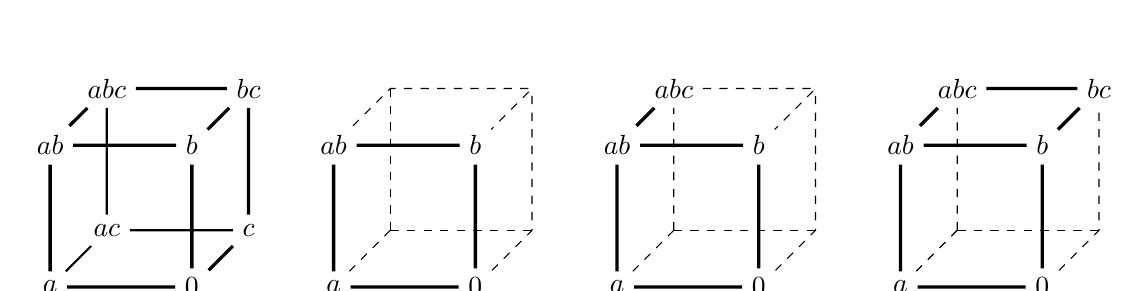
\begin{tikzpicture}[scale=1.8]
\begin{scope}[shift={(0,0)},local bounding box=aa]
    \node (0) at (0, 0) {$0$};
    \node (A) at (-1, 0) {$a$};
    \node (AB) at (-1, 1) {$ab$};
    \node (B) at (0, 1) {$b$};
    \node (C) at (0.4, 0.4) {$c$};
    \node (ABC) at (-0.6, 1.4) {$abc$};
    \node (BC) at (0.4, 1.4) {$bc$};
    \node (AC) at (-0.6, 0.4) {$ac$};

    \draw[very thick] (0) -- (A) -- (AB) -- (B) -- (0) ;
    \draw[very thick] (AB) -- (ABC) -- (BC) -- (B);
    \draw[very thick] (0) -- (C) -- (BC);

    \draw[thick] (AC) -- (A);
    \draw[thick] (AC) -- (ABC);
    \draw[thick] (AC) -- (C);        
\end{scope}

\begin{scope}[shift={(2,0)},local bounding box=bb]
    \node (0) at (0, 0) {$0$};
    \node (A) at (-1, 0) {$a$};
    \node (AB) at (-1, 1) {$ab$};
    \node (B) at (0, 1) {$b$};
    \coordinate (C) at (0.4, 0.4) {}; %{$c$};
    \coordinate (ABC) at (-0.6, 1.4) {}; % {$abc$};
    \coordinate (BC) at (0.4, 1.4) {}; % {$bc$};
    \coordinate (AC) at (-0.6, 0.4) {}; % {$ac$};

    \draw[very thick] (0) -- (A) -- (AB) -- (B) -- (0) ;
    \draw[dashed] (AB) -- (ABC) -- (BC) -- (B);
    \draw[dashed] (0) -- (C) -- (BC);

    \draw[dashed] (AC) -- (A);
    \draw[dashed] (AC) -- (ABC);
    \draw[dashed] (AC) -- (C);        
\end{scope}

\begin{scope}[shift={(4,0)},local bounding box=cc]
    \node (0) at (0, 0) {$0$};
    \node (A) at (-1, 0) {$a$};
    \node (AB) at (-1, 1) {$ab$};
    \node (B) at (0, 1) {$b$};
    \coordinate (C) at (0.4, 0.4) {};% {$c$};%
    \node (ABC) at (-0.6, 1.4) {$abc$};
    \coordinate (BC) at (0.4, 1.4) {};% {$bc$};%
    \coordinate (AC) at (-0.6, 0.4) {};% {$ac$};%

    \draw[very thick] (0) -- (A) -- (AB) -- (B) -- (0) ;
    \draw[very thick] (AB) -- (ABC);
    \draw[dashed] (ABC) -- (BC) -- (B);
    \draw[dashed] (0) -- (C) -- (BC);

    \draw[dashed] (AC) -- (A);
    \draw[dashed] (AC) -- (ABC);
    \draw[dashed] (AC) -- (C);        
\end{scope}

\begin{scope}[shift={(6,0)},local bounding box=dd]
    \node (0) at (0, 0) {$0$};
    \node (A) at (-1, 0) {$a$};
    \node (AB) at (-1, 1) {$ab$};
    \node (B) at (0, 1) {$b$};
    \coordinate (C) at (0.4, 0.4) {};% {$c$};%
    \node (ABC) at (-0.6, 1.4) {$abc$};
    \node (BC) at (0.4, 1.4) {$bc$};
    \coordinate (AC) at (-0.6, 0.4) {};% {$ac$};%

    \draw[very thick] (0) -- (A) -- (AB) -- (B) -- (0) ;
    \draw[very thick] (AB) -- (ABC) -- (BC) -- (B);
    \draw[dashed] (0) -- (C) -- (BC);

    \draw[dashed] (AC) -- (A);
    \draw[dashed] (AC) -- (ABC);
    \draw[dashed] (AC) -- (C);        
\end{scope}
\end{tikzpicture}
\caption{The Boolean lattice on 8 elements represented as a cube, and the 3 Heyting algebras of Figure \ref{fig:3HeytingAlgebras} embedded in this cube.}\label{fig:HAlgsInCubes}
\end{figure}

This hypercube representation immediately tells us that the Hasse diagrams of finite Heyting algebras are made up of lines and squares, and that no two squares can share more than one edge.  Figure \ref{fig:MoreHeytingAlgebras} illustrates a few more proper Heyting algebras, to give a sense of the range of shapes they can take.

\begin{figure}[htbp]
\centering
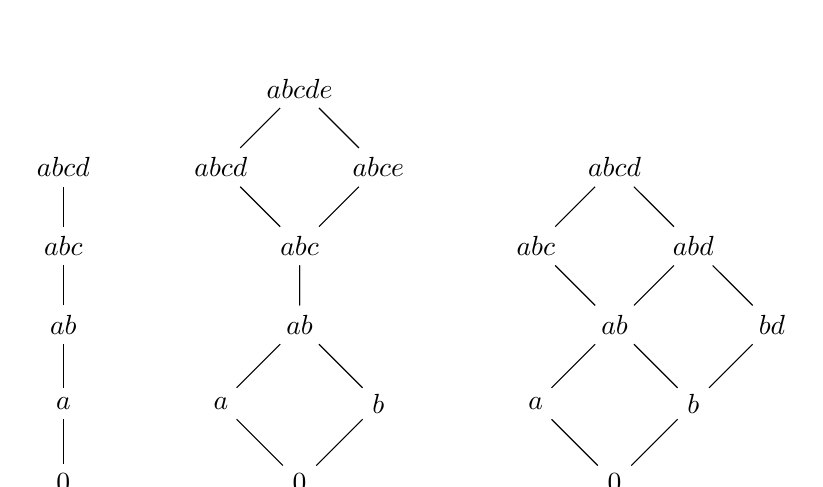
\begin{tikzpicture}[scale=.5]
\begin{scope}[shift={(0,0)},local bounding box=aa]
  \node (ABCD) at (0,8) {$abcd$};
  \node (ABC) at (0,6) {$abc$};
  \node (AB) at (0,4) {$ab$};
  \node (A) at (0,2) {$a$};
  \node (0) at (0,0) {$0$};
  
  \draw (0) -- (A)  -- (AB) -- (ABC) -- (ABCD); 
\end{scope}

\begin{scope}[shift={(6,0)},local bounding box=bb]
  \node (ABCDE) at (0,10) {$abcde$};
  \node (ABCD) at (-2,8) {$abcd$};
  \node (ABCE) at (2,8) {$abce$};
  \node (ABC) at (0,6) {$abc$};

  \node (AB) at (0,4) {$ab$};
  \node (A) at (-2,2) {$a$};
  \node (B) at (2,2) {$b$};
  \node (0) at (0,0) {$0$};
  
  \draw (0) -- (A)  -- (AB) -- (ABC) -- (ABCD) -- (ABCDE); 
  \draw (0) -- (B) -- (AB) -- (ABC) -- (ABCE) -- (ABCDE);
\end{scope}

\begin{scope}[shift={(14,0)},local bounding box=cc]
  \node (ABCD) at (0,8) {$abcd$};
  \node (ABC) at (-2,6) {$abc$};
  \node (ABD) at (2,6) {$abd$};
%  \node (AC) at (-4,4) {$ac$};
  \node (AB) at (0,4) {$ab$};
  \node (BD) at (4,4) {$bd$};
  \node (A) at (-2,2) {$a$};
  \node (B) at (2,2) {$b$};
  \node (0) at (0,0) {$0$};
  
  \draw (0) -- (A)  -- (AB) -- (ABC) -- (ABCD); 
  \draw (0) -- (B) -- (AB) -- (ABD) -- (ABCD);
%  \draw (A) -- (AC) -- (ABC);
  \draw (B) -- (BD) -- (ABD);
  \end{scope}



\end{tikzpicture}
\caption{Some more Heyting algebras.  Every chain forms a Heyting algebra (in which $\NOT x = 0$ for every element).  Heyting algebras can contain single edges between squares, as well as at the top and bottom.  Heyting algebras can be asymmetric.}\label{fig:MoreHeytingAlgebras}
\end{figure}



%\begin{table}[h]
%\centering
%\begin{tabular}{c|ccccc}
%$\IMPLIES$	& T & 2 & 3 & 4 & 0\\
%\hline
%T	&	T & 2 & 3 & 4 & 0	\\
%2	&	T & T & 3 & T & 3	\\
%3	&	T & 2 & T & T & 2	\\
%4	&	T & 2 & 3 & T & 0	\\
%0	&	T & T & T & T & T	\\
%\end{tabular}
%%
%\quad
%%
%\begin{tabular}{c|ccccc}
%$\AND$	& T & 2 & 3 & 4 & 0\\
%\hline
%T	&	T & 2 & 3 & 4 & 0	\\
%2	&	2 & 2 & 0 & 2 & 0	\\
%3	&	3 & 0 & 3 & 3 & 0	\\
%4	&	4 & 2 & 3 & 4 & 0	\\
%0	&	0 & 0 & 0 & 0 & 0	\\
%\end{tabular}
%%
%\quad
%%
%\begin{tabular}{c|ccccc}
%$\OR$	& T & 2 & 3 & 4 & 0\\
%\hline
%T	&	T & T & T & T & T	\\
%2	&	T & 2 & 4 & 4 & 2	\\
%3	&	T & 4 & 3 & 4 & 3	\\
%4	&	T & 4 & 4 & 4 & 4	\\
%0	&	T & 2 & 3 & 3 & 0	\\
%\end{tabular}
%\end{table} 




\subsection{Heyting algebras from preorders}

Another way to specify a Heyting algebra, which will be important in a later section, is to derive it as the lattice of upward closed sets of a preorder.  Let's unpack these terms.

A \terminology{preorder} is a binary relation on a set that is both reflexive and transitive, but need not be symmetric or antisymmetric.  We usually write the relation as $\leq$.

A subset $S$ of a preorder $(W, \leq)$ is \terminology{upward closed} 
if $x \in S$ and $x \leq y$ implies $y \in S$.  That is, if $S$ contains $x$ then it also contains every element of $W$ ``above'' $x$ in the preordering.  We will call an upward closed sets \emph{upsets} for short.  We will write $\uparrow x$ for the set of elements above $x$, i.e. $\uparrow x \DefinedAs \setSuchThat{y}{x \leq y}$, and we will call this the \emph{principal upset on $x$}.  An arbitrary upset is then a union of principal upsets.\footnote{
Trivially, the upset $S$ is the union $\bigcup_{s \in S} \uparrow S$, but there may be a smaller subset of $S$ that also serves as a base in this way (and a finite upset will always have a proper subset that serves as base).
}

Since upsets of $W$ are subsets of $W$, we can order them by subset inclusion.  We will now prove that this ordering on upsets makes then into a Heyting algebra.

\begin{Theorem}
The set of upsets on any preorder $(W, \leq)$, ordered by inclusion, form a Heyting algebra.
\end{Theorem}
\begin{Proof}
Let $(W, \leq)$ be a preorder.  We need to prove that the upsets of $(W, \leq)$ are closed under intersection and union, thus forming a lattice; that this lattice is bounded; and that we can define the $\to$ operation on lattice elements.  %
\begin{enumerate}[(a)]
\item If $P$ and $Q$ are upsets then for any element $i \in W$, 
\[
i \in P \intersect Q 
\iff
i \in P \mbox{ and } i \in Q
\]
Thus for any $j \geq i$, we have $j \in P$ and $i \in Q$, since $P$ and $Q$ are upsets, and thus $j \in P \intersect Q$.  Thus $P \intersect Q$ is also an upset.

\item If $P$ and $Q$ are upsets then for any element $i \in W$, 
\[
i \in P \union Q 
\iff
i \in P \mbox{ or } i \in Q
\]
Thus for any $j \geq i$, we either have $j \in P$ or $i \in Q$, since $P$ and $Q$ are upsets; in either case, $j \in P \union Q$.  Thus $P \union Q$ is also an upset.

\item The whole set $W$ itself is upward closed, and contains every upset as a subset; thus $W$ is the maximal element in the lattice.

\item The empty set $\varnothing$ is (trivially) upward closed, and is contained in every upset as a subset; thus $\varnothing$ is the minimal element in the lattice.

\item For upsets $P$ and $Q$, let 
\[
P \to Q
\DefinedAs
\setSuchThat{i \in W}{\uparrow i \subseteq \bar{P} \union Q}
\]
where $\bar{P} = W\setminus P$.  We will now prove that this satisfies the definition of $\to$ for a Heyting algebra, i.e. that it is the maximal upset $S$ such that $P \intersect S \subseteq Q$.
\begin{enumerate}[(i)]
\item First, $P \to Q$ is an upset: if 
$i \in P \to Q$ then $\uparrow i \subseteq \bar{P} \union Q$, and so for any $j \geq i$ we have ${\uparrow j} \subseteq {\uparrow i} \subseteq \bar{P} \union Q$, and thus $j \in P \to Q$.
%
\item Next, we prove that $P \intersect (P \to Q) \subseteq Q$.  Let 
$i \in P \intersect (P \to Q)$, so 
$\uparrow i \subseteq \bar{P} \union Q$, and so
$i \in \bar{P} \union Q$ (since the preorder relation is reflexive).  Thus 
\[
i \in (\bar{P} \union Q) \intersect P
= (\bar{P} \intersect P) \union (Q \intersect P)
= (Q \intersect P)
\]
by distributivity and the definition of $\bar{P}$.  Thus any $i$ in $P \intersect (P \to Q)$ is also in $Q$.
%
\item Finally, we prove that $P \to Q$ is the maximal such upset.  Let $X$ be an upset satisfying $X \intersect P \subseteq Q$.  Then we need to prove $X \subseteq (P \to Q)$.  Since $X$ is an upset, for any $x \in X$ we have $\uparrow x \subseteq X$.  But 
\[
X \intersect P \subseteq Q 
\iff
X \intersect P \intersect \bar{Q} = \varnothing
\iff
X \subseteq \bar{P} \intersect Q
\]
and so for any $x \in X$, $\uparrow x \subseteq X \subseteq \bar{P} \intersect Q$, and thus $x \in P \to Q$.
\end{enumerate}
\end{enumerate}
\end{Proof}

This gives us a useful way of constructing Heyting algebras -- we just give a preorder on some set and then order its upsets by subset inclusion.  As we'll see later, we can use this when we want to build Heyting algebra models of constructive logic satisfying certain properties.



\subsection{Logic with Heyting algebras}

Just as Boolean algebras provide the appropriate truth values for classical logic, Heyting algebras provide the appropriate truth values for constructive logic.


In Section \ref{sec:Models-TruthTables} we built a truth table for a formula in which each row corresponded to a way of assigning to each variable a truth value in the Boolean algebra $\{T, F\}$.  We can do exactly the same thing if we replace that Boolean algebra with any Heyting algebra -- since the usual logical operations are defined on a Heyting algebra, any assignment of values to the variables leads to a unique value for the formula itself.

We said that a formula is provable in CPL iff it is true under any assignment into $\{T, F\}$.  What is the corresponding result for constructive logic?  Which Heyting algebra plays the same role?  Unfortunately there is \emph{no} single Heyting algebra that serves the purpose.\footnote{As G\"{o}del proved in (1932).}  
However, what is true is that a formula is provable in constructive propositional logic iff it is a tautology -- i.e. gets the maximal value -- in \emph{every} Heyting algebra.  That means that if there is any assignment of values in any Heyting algebra that results in the formula getting a non-maximal value, then that formula is not provable constructively.  Thus we can still use truth tables to find  counterexamples to constructively invalid formulae.

As an example, consider again the formula 
$\NOT (P \AND Q) \IMPLIES ((\NOT P) \OR (\NOT Q))$.  We can evaluate this in any Heyting algebra, of course, but some will be more useful than others.  If we choose a Boolean algebra the formula will always get maximal value.  Likewise if we evaluate it in the 3-element chain.  But  in the 5-element Heyting algebra illustrated in Figure \ref{fig:3HeytingAlgebras} we can get a counterexample.  Since there are two variables we have $5^2=25$ rows to calculate, so we won't display the whole table -- but we don't need to.  To show that this formula is not constructively valid we just need to exhibit a single counterexample, i.e. a single row in which the formula does not have the maximal value $abc$ in that Heyting algebra, such as:
\begin{table}[h]
\centering
\begin{tabular}{c c|c c c}
P &	Q & $\NOT(P \AND Q)$ &	$(\NOT P) \OR (\NOT Q)$ &	$\NOT (P \AND Q) \IMPLIES ((\NOT P) \OR (\NOT Q))$ \\
\hline
a & b & 1 & ab & ab
\end{tabular}
\end{table}\\
That this is in fact a counterexample is easy to verify -- we simply have to evaluate the formula with the given values for the variables.  A Heyting algebra counterexample therefore provides a simple, compact, and easily verified demonstration that a given formula is not a tautology of constructive logic (and thus, via the Deduction theorem, that a given argument is not constructively valid).



\subsection{Building specific Heyting algebra counterexamples}

Although they are easy to verify, Heyting algebra counterexamples may not be easy to find.  For one thing, we do not know in advance \emph{which} Heyting algebra to evaluate into.  Then for any Heyting algebra we need to work out the entire truth table, which is a mechanical but tedious process.  It would be better, then, to have some means of producing counterexamples from formulae directly, or of demonstrating directly when a formula does not have a counterexample.

Ideally, what we would like (assuming we knew what Heyting algebra we should work in) is to construct a counterexample \emph{backwards}: starting with a non-maximal value in the right-most column of the truth table, we could then work from right to left, filling in the values that the preceding columns must take, until we eventually get to the left-most column containing the values of the variables.  


Of course, there are many factors that complicate matters.  First, we don't know which Heyting algebra we should be working in, and we don't yet even have a principle bounding the size of the Heyting algebras we need to consider.  Second, we don't know which non-maximal value the formula should take.  (For that matter, we don't even know in advance whether the formula has a counterexample at all -- that's what this process is supposed to find out.)  Then, for any given value in one column, there may be multiple compatible values that we could put in the preceding columns: for example, in two-valued Boolean logic, if we put $T$ in a column headed $A \OR B$ then there are 3 possible pairs of values we could assign to $A$ and $B$ that are compatible with this.  We would therefore need a \emph{branching} process, exploring each of these possibilities in parallel.

These various obstacles appear to make such a ``reverse-engineering'' of a counterexample unfeasible (or perhaps no less work than simply working out the whole truth table for a few Heyting algebras and hoping for some principle to guide us to the right one).  
However, a process based upon essentially this idea
 -- although with some major alterations! -- can be made to work, and this is the procedure we'll describe in the remainder of this section.

Rather than choosing the Heyting algebra in advance we will build it up indirectly by constructing a preorder by following certain rules depending upon the structure of the formula we are trying to disprove.  At the end of the procedure we will either have such a preorder, from which we can then obtain a Heyting algebra via the procedure of Section \ref{}, or we will find that no such preorder can be constructed.  In the latter case we wil have shown that there are no counterexamples to the formula, and thus the formula is a constructive tautology (and we should therefore direct our efforts into finding a constructive proof for it instead!)


\subsection{The rules of countermodel construction}

We want to define a preorder, so that we can obtain a Heyting algebra from it as its collection of upsets.  We also want to obtain an evaluation function from propositional variables and formulae into the Heyting algebra.  In particular, we want this evaluation to give a non-maximal value to the formula for which we are trying to give a countermodel.  So now we need to define a set of rules that will produce such a preorder for any formula that has a countermodel (i.e. any formula that is not a tautology of constructive logic).

If values in the Heyting algebra correspond to upsets in the preorder, then the valuation into the Heyting algebra, $h: F \to H$ should come from a valuation $\omega$ into the upsets of the preorder.  That is, for each formula $A$, $\omega(A)$ is an upward closed subset of the preorder.  It will also be useful to have a name for the complement of $\omega(A)$ in $W$, which we will denote $\bar{\omega}(A)$.


The valuation $h$ into the Heyting algebra that we obtain must be internally consistent -- for example, for any conjunction $A \AND B$ we must have $h(A \AND B) = h(A) \glb h(B)$.  If we pick values of $\omega$ arbitrarily then of course we can't expect this to hold, so we must impose rules on $\omega$ to guarantee consistency among values.  Specifically, we've seen in Section \ref{HAlgs-from-preorders} how the values must relate to one another: for all formulae $A$ and $B$,
\begin{itemize}
\item $\omega(A \AND B) \DefinedAs \omega(A) \intersect \omega{B}$
\item $\omega(A \OR B) \DefinedAs \omega(A) \union \omega{B}$
\item $\omega(A \to B) \DefinedAs 
\setSuchThat{i \in W}{\uparrow i \subseteq \bar{\omega}(A) \union \omega(B)}$
\end{itemize}
(where the latter condition follows from the fact that the upset corresponding to $A \to B$ must be the maximal upset $S$ such that $\omega(A) \intersect S \subseteq \omega(B)$.)

As usual, we define $\NOT A$ as $A \to \ABSURDITY$, where $\ABSURDITY$ is a contradictory proposition that is never true -- i.e. $\omega(\ABSURDITY) = \varnothing$.  Thus
\begin{itemize}
\item $\omega(\NOT A) \DefinedAs 
\setSuchThat{i \in W}{\uparrow i \subseteq \bar{\omega}(A)}$
\end{itemize}
Note that $\omega(\NOT A)$ is in general \emph{not} equal to $\bar{\omega}(A)$, but is always a subset of it.\footnote{
Proof sketch: if $i \in \omega(\NOT A)$ then $\uparrow i \subseteq \bar{\omega}(A)$, and we always have $i \in \uparrow i$, so 
$i \in \omega(\NOT A) \subseteq \bar{\omega}(A)$.  But for the converse dirction, $j \in \bar{\omega}(A)$ is not sufficient to guarantee $\uparrow j \subseteq \bar{\omega}(A)$, so in general $j \not\in \omega(\NOT A)$ and thus $\bar{\omega}(A) \not\subseteq \omega(\NOT A)$.
}
That is, $\omega(\NOT A) \intersect \omega(A) = \varnothing$, but 
$\omega(\NOT A) \union \omega(A) \neq W$, as we would expect for an intuitionistic logic.

We noted above that the whole preorder, being an upset, serves as the maximal element $1$ of the Heyting algebra.  Thus if the preorder has a root element -- i.e. a world $w_0$ such that $\forall w \in W,\, w_0 \leq w$ -- then any formula $A$ with $w_0 \in \omega(A)$ must (by the requirement that $\omega(A)$ be an upset) have $\omega(A) = W$, and therefore gets value $1$ in the Heyting algebra.  Conversely, to ensure that a formula $A$ does \emph{not} get maximal value in the Heyting algebra, we just need to ensure that $w_0 \not\in \omega(A)$.  This therefore gives our final two conditions when building a counterexample to $A$: ensure that the preorder has a root world $w_0$, and set $w_0 \not\in \omega(A)$.


So, given a formula $\phi$ that we wish to show is not a tautology, we  need to construct a rooted preorder $(W, \leq, w_0)$ and an evaluation function $\omega: F \to 2^W$ that assigns to each formula\footnote{
Specifically, to each formula using the same propositional variables as $\phi$.} 
an upward-closed subset of $W$, ensuring that $\omega$ obeys the rules above, and in which $w_0 \not\in \omega(\phi)$.  In the next section we will see the procedure that allows us to carry out this construction if it it possible.



%Another way to encode the same information is via a function $\nu: W \times F \to \set{0,1}$, defined by
%\[
%\nu(i, A) = 1 \quad \iff \quad i \in \omega(A)
%\]
%To ensure that the sets of worlds assigned to each formula are upward closed, we must impose a condition: if $\nu(i,A) = 1$ then for all $j \geq i$ in the preorder, $\nu(j,A) = 1$.

%For $\AND$ and $\OR$ the rules are obvious: for all $i \in W$, and all formulae $A$ and $B$,
%\[
%\nu(i,A \AND B) = 1 \quad \mbox{ iff } \quad 
%\nu(i,A) = 1 \mbox{ and } \nu(i,B) = 1
%\]
%\[
%\nu(i,A \OR B) = 1 \quad \mbox{ iff } \quad 
%\nu(i,A) = 1 \mbox{ or } \nu(i,B) = 1
%\]
%Equivalently, we can express these as sums and products of values:
%\begin{align*}
%\nu(i,A \AND B) &\DefinedAs 
%\nu(i,A) \times \nu(i,B)
%\\
%\nu(i,A \OR B) &\DefinedAs
%\nu(i,A) + \nu(i,B) - \nu(i,A) \times \nu(i,B)
%\end{align*}





%Part of the problem here is that when we do constructive logic all we know at a given time is which types we have terms for -- we have no way of positively recording the fact that we \emph{don't} have a term of a given type.  The mere omission of a term from the list of things we're given is not sufficient, since it may be possible to construct such a term from the things we are given and we have simply not yet done so.  That is, the fact that a term has not been constructed in a given context is not evidence that it \emph{cannot} be constructed in that context.  But it is precisely the latter that we need to demonstrate in order to show that a particular construction is not possible.  We therefore need a new approach to studying constructive arguments, in which both the presence and absence of terms can be actively recorded.
%
%In a constructive model, the failure to record that a term is present does not correspond to that term's being absent.  We models we require must therefore be \emph{classical}.  
%
%
%\subsubsection{Definition of Kripke models}
%
%A \terminology{Kripke frame} is a pair of a non-empty set $W$, whose elements we call \terminology{worlds}, and a binary relation $R$ on $W$, which we call \terminology{accessibility}.  For the most general Kripke frame we assume no particular properties of $R$.  However, for present purposes we will restrict attention to Kripke frames whose accessibility relations are \emph{reflexive} and \emph{transitive} (i.e. which are \emph{preorders}).  We therefore write the accessibility relation as $\leq$.
%
%An \terminology{intuitionistic Kripke model} is then a Kripke frame along with a relation $\makestrue$ between worlds and expressions of our language, such that:
%\begin{samepage}
%\begin{itemize}
%\item $w \makestrue A \AND B$ iff $w \makestrue A$ and $w \makestrue B$
%\item $w \makestrue A \OR B$  iff $w \makestrue A$ or  $w \makestrue B$
%\item $w \makestrue A \IMPLIES B$ iff for all $u \geq w$, $u \makestrue A$ implies $u \makestrue B$
%\item $w \not \makestrue \ABSURDITY$
%\item for any propositional variable, if $w \makestrue p$ and $w \leq u$ then $u \makestrue p$
%\end{itemize}
%\end{samepage}
%











%\newpage

%\setcounter{section}{6}
%\section{Recursive Types}
\label{sec:DataTypes}

\subsection{Defining a new type in a new way}
\label{sec:NaturalNumbers-NewTypeNewWay}

In Section \ref{} we introduced into the type theory two ways to form new types from old ones: the product 
$\type{A} \x \type{B}$ and the coproduct
$\type{A} \+ \type{B}$.
In each case we had to specify the \emph{term constructors} for the new type, i.e. the basic functions that give terms of this type as their outputs.  The term constructor for product takes one $\term{a}:\type{A}$ and one $\term{b}:\type{B}$ and returns a pair 
$(\term{a}, \term{b}):\type{A} \x \type{B}$.  The coproduct type has two constructors, namely $\inl: \type{A} \to \type{A} \+ \type{B}$ and  
$\inr: \type{B} \to \type{A} \+ \type{B}$.

We also introduced the finite types (Section \ref{}), whose constructors don't take any input from any other type, they just each produce a single specific term of the type (e.g. for the type \type{2} the constructors are $\term{0}_{\type{2}}:\type{2}$ and $\term{1}_{\type{2}}:\type{2}$).  We can think of these ``no-input constructors'' as (being provided by) functions into their corresponding types as well, since we can take the input type to be \type{1}, the Unit type.  Since this has only one term, $\ast:\type{1}$, any function $\term{f}: \type{1} \to \type{A}$ just picks out a single term $\term{f}(\ast):\type{A}$.  Thus any constructor, whether it depends upon inputs or just picks out a term of the type, can be given as a function into the type.\footnote{
In a slight abuse of notation, we will use the same name for a function $\type{1} \to \type{A}$ and for the term of $\term{A}$ that it picks out.  These are of course different entities belonging to different types, but since they are effectively interchangeable no harm will come from this convenience.
}

In this section we'll introduce types that are defined \emph{recursively}.  Whereas the constructors for the types we've defined before always take their inputs from \emph{other} types, a \terminology{recursive type} 
\type{R} has at least one constructor taking input from \type{R} itself.


Recursive types include some of the most important used structures in computer science 
(where they are more commonly called ``recursive data types''), such as trees and lists.  They also include a type that's very important in mathematics: the natural numbers, $\NN$.



\subsection{Lists}

A \terminology{list} is a finite ordered collection of zero or more terms of some given type \type{A} in which repetition is allowed.  For each type \type{A} there is therefore a type \emph{lists of terms of type \type{A}}, which we call $\List{\type{A}}$.

Since we allow a collection of zero elements to constitute a list, there is always a term $\Nil: \List{\type{A}}$, which we call the ``empty list''.\footnote{
Strictly we ought to put a subscript on $\Nil$ to indicate which type it belongs to, since 
$\Nil_{\type{A}}:\List{\type{A}}$
is a distinct term from 
$\Nil_{\type{B}}:\List{\type{B}}$, but for convenience we won't.
}

Since lists are ordered collections, any list that is not empty must contain a \emph{first} element, which is a term of \type{A}.  The remainder of the list is then also an ordered collection of zero or more terms of \type{A}, i.e. another list.  Thus any non-empty list in $\List{\type{A}}$ must be built from some $\term{a}:\type{A}$ and some $\term{L}:\List{\type{A}}$.

This gives us our two constructors for the type $\List{\type{A}}$:
\begin{align*}
\Nil&: \type{1} \to \List{\type{A}}  \\
cons&: \type{A} \x \List{\type{A}} \to \List{\type{A}}
\end{align*}
There are many different notations used for lists in mathematics and computer science.  In computer science the second constructor is traditionally called ``$cons$'' (short for ``constructor''\footnote{
This gives some indication of how important lists are in some programming languages!  In particular in one of the first functional programming languages \emph{Lisp}, which is short for ``LISt Processing''.
}), and $cons(\term{a}, \term{L})$ is often written as $\term{a}::\term{L}$.  However, this ``double colon'' notation threatens to clash with our notation for terms belonging to types, so we will instead use the notation $\ListOf{\term{a}}{\term{L}}$.  If we know that all the elements of the list are some particular terms 
\term{p}, \term{q}, \term{r}, and \term{s} of \type{A} (in that order) we may write the list as 
$[\term{p}, \term{q}, \term{r}, \term{s}]$.
We will also often use the traditional name $\term{as}$ for a list of type $\List{\type{A}}$ (which we read as the plural of \term{a}), and likewise $\term{bs}:\List{\type{B}}$, etc.

\subsection{Equations for Lists}

Since every list is of finite length, every list must either be of length 0, or length 1, or length 2, or \ldots etc.  This suggests the equation
\[
\List{\type{A}} \simeq \type{1} \+ \type{A} \+ (\type{A} \x \type{A}) \+ (\type{A} \x \type{A} \x \type{A}) \+ \ldots
\]
We can interpret the $\simeq$ sign here as $\dashv \; \tstile$, in the sense that if we have a term of one side then we can use it to construct a term of the other.

We can go further in approaching something that looks like arithmetic.  As we discussed above, a term of \type{A} is equivalent to a function of type $\type{1} \to \type{A}$.  We can write this as 
\[
\type{A} \;\simeq\; \type{1} \to \type{A}
\]
Similarly, a term of type $(\type{A} \x \type{A})$ is equivalent to a function of type $\type{2} \to \type{A}$; any such function $\term{f}$ picks out two values 
$f(\term{0}_{\type{2}}):\type{A}$ and 
$f(\term{1}_{\type{2}}):\type{A}$ and therefore corresponds to the term 
$(f(\term{0}_{\type{2}}),
f(\term{1}_{\type{2}})): \type{A} \x \type{A}$.  We can write this as
\[
\type{A} \x \type{A} \;\simeq\; \type{2} \to \type{A}
\]

We can of course extend the same argument: any product of the form 
$\type{A} \x \type{A} \x \ldots \x \type{A}$ with $n$ instances of $\type{A}$ is equivalent to a function $\type{n} \to \type{A}$, where \type{n} is the finite type containing $n$ terms.  That is,
\[
\underbrace{\type{A} \x \type{A} \x \ldots \x \type{A}}_\text{$n$ \type{A}s} 
\;\simeq\; \type{n} \to \type{A}
\]

But we can go further again.  If we use the common alternative notation $\type{Y}^{\type{X}}$ for the function type $\type{X} \to \type{Y}$ then we can write the above correspondences as
\begin{align*}
\type{A} \;&\simeq\; \type{A}^{\type{1}}
\\
\type{A} \x \type{A} \;&\simeq\; 
\type{A}^{\type{2}}
\\
\underbrace{\type{A} \x \type{A} \x \ldots \x \type{A}}_\text{$n$ \type{A}s} 
\;&\simeq\; 
\type{A}^{\type{n}}
\end{align*}
This is just a literal translation of the notation for exponentials!

Using this notation, we can re-write the equation for lists as
\[
\List{\type{A}} 
\;\simeq\;
\type{1} \+ \type{A}^{\type{1}} \+ \type{A}^{\type{2}} \+ \type{A}^{\type{3}} \ldots
\]
Thus $\List{\type{A}}$ looks like a \terminology{formal power series} in the ``variable'' \type{A}.


There's another equation we can write involving $\List{\type{A}}$.  Since the two constructors for $\List{\type{A}}$ take respectively a term of \type{1} or a term of $\type{A} \x \List{\type{A}}$, if we have a term of either type we can produce a term of $\List{\type{A}}$ by applying the appropriate constructor.  Thus we can define a function of type
\[
(\type{1} \+ \type{A} \x \List{\type{A}}) \to \List{\type{A}}
\]
But likewise given any list we can either decompose it (if it is not empty) into its first element and the remainder, or (if it is empty) just produce the term $\ast:\type{1}$.  We can therefore also define a function of type
\[
\List{\type{A}} \to (\type{1} \+ \type{A} \x \List{\type{A}})
\]
We therefore have the equation 
\[
\List{\type{A}} \;\simeq\; \type{1} \+ \type{A} \x \List{\type{A}}
\]
If we were doing algebra and were presented with the equation
\[
L(x) = 1 + x \times L(x)
\]
we could solve for $L(x)$ to get $L(x) = 1 + x + x^2 + x^3 \ldots$ which is exactly parallel to the equation we wrote for $\List{\type{A}}$ above!  There's clearly an interesting connection between this recursive type and this formal power series.  In subsequent sections we will develop this connection further.


\subsection{Binary Trees}

A \terminology{binary tree} over \type{A} is a recursively-defined structure\footnote{
There are many different variants of binary trees one could define.  For example, we could allow the ``empty binary tree'' with no elements, or we could label the internal nodes of the tree with terms of \type{A} (or of some other type \type{B}).  Each such variant constitutes a different type with slightly different constructors.  
Exercise: how would we modify the constructors to accomodate the variants described above?
} 
consisting of either a single term of type \type{A} or a pair of binary trees over \type{A} which we call the \terminology{left and right subtrees}.  These form a type, $\BTree{\type{A}}$.

The constructors of $\BTree{\type{A}}$ are therefore
\begin{align*}
Leaf&: \type{A} \to \BTree{\type{A}}
\\
Node&: \BTree{\type{A}} \x \BTree{\type{A}} \to \BTree{\type{A}}
\end{align*}

By an argument parallel to the one given in the previous section, we have a correspondence
\[
\BTree{\type{A}} 
\;\simeq\;
\type{A} \x \BTree{\type{A}} \x \BTree{\type{A}}
\]
or
\[
\BTree{\type{A}} 
\;\simeq\;
\type{A} \x (\BTree{\type{A}})^{\type{2}}
\]
If we treat this as an equation to be solved, namely
\[
b(x) = x \times (b(x))^2
\]
we find a solution
\[
b(x) = \frac{1 - \sqrt{1 - 4x}}{2}
\] 
whose Taylor expansion is
\[
b(x) = x + x^2 + 2x^3 + 5x^4 + 14x^5 + 42x^6 + \ldots
\]
Interpreting this back into types (as we did in the case of Lists above) we get
\[
\BTree{\type{A}} 
\;\simeq\;
\type{A} \+ 
(\type{A}^{\type{2}}) \+ 
(\type{2}\x \type{A}^{\type{3}}) \+ 
(\type{5}\x \type{A}^{\type{4}}) \+ 
(\type{14}\x \type{A}^{\type{5}}) \+ 
(\type{42}\x \type{A}^{\type{6}}) \+ \ldots
\]
The coefficients here are the \emph{Catalan numbers}, which count the  binary trees on $n$ leaves.  The above equation says that a binary tree whose leaves are labelled with terms of \type{A} is either a single term of \type{A}, or an ordered pair of terms of \type{A}, or one of the two binary trees with 3 leaves plus an ordered triple of terms of \type{A}, or \ldots  So by manipulation of equations involving the type $\BTree{\type{A}} $ we have arrived at a correct description of that type!\footnote{
For more on this, see John Baez's various articles on ``structure types''.
}

\newpage
\section{Natural numbers}
\label{sec:NaturalNumbers}

The type we're defining here is, of course, the \terminology{natural numbers}, $\type{\NN}$.  We'll call the no-input term constructor 
$\term{0}_{\type{\NN}}:\type{\NN}$.  
The other term constructor takes a term of $\type{\NN}$ and returns a new term.  It is therefore naturally interpreted as the \terminology{successor} operation, so we call it $s$.  
Thus the terms of $\type{\NN}$ can be written as
\[
\begin{cases}
\term{0}_{\type{\NN}}:\type{\NN}
\\
s(\term{n}):\type{\NN}\mbox{ for some }\term{n}:\type{\NN}
\end{cases}
\] 
The first few natural numbers are therefore $\term{0}_{\type{\NN}}$, 
$s(\term{0}_{\type{\NN}})$, $s(s(\term{0}_{\type{\NN}}))$, $s(s(s(\term{0}_{\type{\NN}})))$, and so on.
But rather than writing out numbers in this unary representation, we'll generally switch to the usual numerals, e.g. writing $3$ for $s(s(s(\term{0}_{\type{\NN}})))$.\footnote{
Context should make it clear when we're talking about \emph{numbers}, which are terms of type \type{\NN}, rather than \emph{types} like \type{0} and \type{2}, which are not directly related to \type{\NN} at all.
}  (Note that we won't put a subscript `\NN' on these numerals, to avoid cluttering up the notation.) 


\subsection{Defining addition on $\type{\NN}$}
\label{sec:NaturalNumbers-AdditionOnN}

Having defined natural numbers, we want to be able to do basic arithmetic on them.  Let's first see how to define addition.

The addition function will take two natural numbers and return another.  We can therefore define it by a (curried) function
\[
\term{add}:\NN \to (\NN \to \NN)
\]
where for any $\term{x}:\type{\NN}$, the function
$\term{add}_{\term{x}}: \type{\NN} \to \type{\NN}$
takes any $\term{m}:\type{\NN}$ and adds \term{x} to it.\footnote{
TODO: Spell this out in more detail with a particular example.  Mention commutativity and link ahead to the worked example.
}
To define \term{add} we therefore need to know what function  $\term{add}_{\term{x}}:\NN \to \NN$ is  for each 
$\term{x}:\type{\NN}$.

We can immediately see that $\term{add}_{ \term{0}_{\type{\NN}}}$ is the identity function 
$ \term{m} \mapsto \term{m}$, since adding zero to any number leaves it unchanged.  

By the definition of the natural numbers given above, any other natural number aside from $\term{0}_{\type{\NN}}$
must be of the form $s(\term{n})$ for some 
$\term{n}:\type{\NN}$.  We can use this fact, and the fact that 
$(1+n) + m = 1 + (n + m)$, to 
give a \terminology{recursive} definition of addition: to add $s(\term{n})$ to some number \term{m} we first add \term{n} to it, and then take the successor of the result.  This allows us to complete the definition:
for any $\term{n}:\type{\NN}$, 
the function $\term{add}_{s(\term{n})}$ is defined as:
\[
\term{add}_{s(\term{n})}(\term{m}) \DefinedAs
s(\term{add}_{\term{n}}(\term{m}))
\]

  The full definition of the addition function is therefore:
\begin{align*}
\term{add}(\term{0}_{\type{\NN}})(\term{m}) &\DefinedAs \term{m}
\\
\term{add}(s(\term{n}))(\term{m}) &\DefinedAs
s(\term{add}(\term{n})(\term{m}))
\end{align*}
This is a \emph{recursive} definition in the sense that it gives the definition of the sum of more complex terms 
(i.e. $s(\term{n})$ and $\term{m}$)
via the sum of less complex ones
(i.e.~$\term{n}$~and~$\term{m}$).\footnote{
TODO: Explain explicitly that \term{add} mirrors the structure of $\NN$ itself, since each $add_n$ function is defined in terms of the next smaller one, down to the base case.  This is foreshadowing the general idea of structural recursion and the definition of the recursor.
}



\subsection{Pattern matching}
\label{sec:NaturalNumbers-PatternMatching}

We call this style of function definition \terminology{pattern matching}.  Let's see how it works in the present example.

When we apply the \term{add} function to a pair of inputs \term{a} and \term{b}:
\begin{enumerate}[(i)]
\item we will compare the expression 
$\term{add}(\term{a})(\term{b})$ against each of the patterns above; 
\item it will match against \emph{exactly one} of those patterns -- i.e. \term{a} will be either $\term{0}_{\type{\NN}}$ or $s(\term{n})$ for some $\term{n}:\type{\NN}$;
\item the line that matches serves as the definition of $\term{add}(\term{a})(\term{b})$ in this instance;
\item each variable on the left side of that line takes a unique value in matching $\term{add}(\term{a})(\term{b})$;
\item the value of $\term{add}(\term{a})(\term{b})$ is therefore given by the right side of that line, with the variables taking those same values.
\end{enumerate}

Of course, we've seen the pattern matching style of definition before, when defining things by case analysis -- for example on coproducts, or on the type \type{2}.  
For definitions on \type{2} the pattern matching is trivial, since the only part of the pattern that varies from one case to another is whether we're dealing with $\term{0}_{\type{2}}$ or $\term{1}_{\type{2}}$.  
Pattern matching for coproducts is slightly more sophisticated -- a term of the coproduct $\type{A} \+ \type{B}$ is either of the form $\inl(\term{a})$ for some $\term{a}:\type{A}$ or of the form $\inr(\term{b})$ for some $\term{b}:\type{B}$, so we not only have to match against which of these two options we have, but then also match a variable to the given \term{a} or \term{b}, as in step (iv) above.

For natural numbers, pattern matching is just slightly more sophisticated again.  Now the options are $\term{0}_{\type{\NN}}$ or $s(\term{n})$ for some $\term{n}:\type{\NN}$, so first we have to match against which of these two options we have, and then \emph{if} we have $s(\term{n})$ we have to match a variable to the value \term{n}.

In general, definitions given in pattern matching style can be much more complicated than this, with many more than just two patterns to choose between, and more than just one or two variables to match against.  However, in practice, actually using a pattern matching style definition is easy, since we just have to compare the input we're given to each line of the pattern in turn, and confirm whether we have the right number of pieces, each of the right type, as specified by that line.





\subsection{An example of addition}
\label{sec:NaturalNumbers-ExampleAddition}

To make sure we understand it, let's do a simple example in full tedious detail: let's add $2$ and $3$.  %We'll write the numbers as $s(s(\term{0}_{\type{\NN}}))$ and $s(s(s(\term{0}_{\type{\NN}})))$, to make everything explicit.

To evaluate
$\term{add}(2)(3)$ we pattern match against each line of the definition of \term{add}.  $2$ is of the form $s(\term{n})$ for some $\term{n}:\type{\NN}$, so we match the second line, with \term{n} taking the value $1$ and \term{m} taking the value $3$.  The value of $\term{add}(2)(3)$ is therefore 
$s(\term{add}(1)(3))$, and so we need to evaluate $\term{add}(1)(3)$.

To evaluate
$\term{add}(1)(3)$ we pattern match against each line of the definition of \term{add}.  $1$ is of the form $s(\term{n})$ for some $\term{n}:\type{\NN}$, so we match the second line, with \term{n} taking the value $\term{0}_{\type{\NN}}$ and \term{m} taking the value $3$.  The value of our original function application $\term{add}(2)(3)$ is therefore 
$s(s(\term{add}(\term{0}_{\type{\NN}})(3)))$, and so we need to evaluate $\term{add}(\term{0}_{\type{\NN}})(3)$.

To evaluate
$\term{add}(\term{0}_{\type{\NN}})(3)$ we pattern match against each line of the definition of \term{add}, and we find a match at the first line with \term{m} taking the value $3$.  Thus $\term{add}(\term{0}_{\type{\NN}})(3)$ evaluates to $3$.

The value of our original function application $\term{add}(2)(3)$ is therefore $s(s(3))$ -- or, in full, 
$s(s(s(s(s(\term{0}_{\type{\NN}})))))$, 
which is a term of \type{\NN}, and so the evaluation is complete.

As is easily confirmed, if we had instead evaluated $\term{add}(3)(2)$ we would have gone through a different sequence of steps but would have ended up with the same term $s(s(s(s(s(\term{0}_{\type{\NN}})))))$ of $\type{\NN}$.\footnote{We will later be able to prove that addition is commutative -- i.e. that $\term{add}(\term{a})(\term{b})$ equals $\term{add}(\term{b})(\term{a})$ for all $\term{a}:\type{\NN}$ and $\term{b}:\type{\NN}$.  However, we don't yet have all the resources we need to express this, since we currently have no way to say that two terms of a type are the same (i.e. in this case, the same number).  Once we've introduced this new feature to our language in Section~\ref{} we'll return to investigate equations and proofs in arithmetic.
}
 

\subsection{Defining multiplication and exponentiation}
\label{sec:NaturalNumbers-MultiplicationExponentiation}

We have defined addition of natural numbers as repeated succession:
\begin{align*}
\term{add}(\term{0}_{\type{\NN}})(\term{m}) &\DefinedAs \term{m}
\\
\term{add}(s(\term{n}))(\term{m}) &\DefinedAs
s(\term{add}(\term{n})(\term{m}))
\end{align*}

We can use a similar pattern to define multiplication as repeated addition:
\begin{align*}
\term{mult}(\term{0}_{\type{\NN}})(\term{m}) &\DefinedAs \term{0}_{\type{\NN}}
\\
\term{mult}(s(\term{n}))(\term{m}) &\DefinedAs
\term{add}(\term{m})(\term{mult}(\term{n})(\term{m}))
\end{align*}
The first line just says that the product of zero with ny number is zero.  The second line says that $(1+n) \times m = m + (n \times m)$.  Since, as before, any natural number is either $\term{0}_{\type{\NN}}$ or $s(\term{n})$ for some $\term{n}:\type{\NN}$, these two cases are exhaustive and exclusive.  Again we can see by inspection that the call to \term{mult} on the right side of the second line takes a smaller argument than the one we're evaluating, so this will eventually hit the base case and terminate.  Then we're left with a sequence of additions to evaluate, and we've already seen that addition is well defined.  Thus the multiplication function is also well defined.

Let's look at a simple example -- but in much less detail than the example we did for addition!  To evaluate 
$\term{mult}(\term{3})(\term{4})$
we pattern match against the above definition, and we find a match with the second line, with \term{n} taking the value $2$ and \term{m} taking the value $4$.  Thus we need to evaluate
$\term{add}(\term{4})(\term{mult}(\term{2})(\term{4}))$.  To do this we evaluate 
$\term{mult}(\term{2})(\term{4})$, which in turn requires us to evaluate
$\term{mult}(\term{1})(\term{4})$, which finally requires us to evaluate
$\term{mult}(\term{0}_{\type{\NN}})(\term{4})$.  We therefore end up with the sequence of additions, adding three $4$s to $\term{0}_{\type{\NN}}$, which evaluates to $12$, as expected.

Note that, in both addition and multiplication, the recursive part (i.e. the line in which the input is of the form $s(\term{n})$)
involves the evaluation of the same function on a smaller input (respectively, 
$\term{add}(\term{n})(\term{m})$
and 
$\term{mult}(\term{n})(\term{m})$), 
the result of which is then acted upon by another function
(respectively,
$s$ and 
$\term{add}(\term{m})$).

Having defined addition as repeated succession and multiplication as repeated addition, we can go on to define the function we get by repeated multiplication, namely exponentiation.  We will define 
$\term{exp}(\term{n})(\term{m})$ as $m^n$, so that we can use the same pattern as above.  We use the fact that $m^0 = 1$ and $m^{(1+n)} = m \times m^n$:
\begin{align*}
\term{exp}(\term{0}_{\type{\NN}})(\term{m}) &\DefinedAs 1
\\
\term{exp}(s(\term{n}))(\term{m}) &\DefinedAs
\term{mult}(\term{m})(\term{exp}(\term{n})(\term{m}))
\end{align*}
Again, the recursive line here involves a call to \term{exp} with a smaller input, followed by the application of another well-defined function $\term{mult}(\term{m})$.


\subsection{Some other simple functions}
\label{sec:NaturalNumbers-OtherFunctions}

Let's quickly review some other functions on the natural numbers that we can easily define.
\begin{description}
\item[Double] We use the facts that $2\times 0 = 0$ and $2\times (n+1) = 1+1+(2\times n)$
\begin{align*}
\term{double}(\term{0}_{\type{\NN}}) 
&\DefinedAs 
\term{0}_{\type{\NN}}
\\
\term{double}(s(\term{n})) 
&\DefinedAs
s(s(\term{double}(\term{n})))
\end{align*}
%
\item[Factorial]  $0! = 1$; $(n+1)! = (n+1) \times n!$
\begin{align*}
\term{fact}(\term{0}_{\type{\NN}}) 
&\DefinedAs 
1\\
\term{fact}(s(\term{n})) 
&\DefinedAs
\term{mult}(s(\term{n}))(\term{fact}(\term{n}))
\end{align*}
%
\item[Triangular] The $n^{\mbox{th}}$ triangular number, $1+2+3+ \ldots +n$
\begin{align*}
\term{sum-to}(\term{0}_{\type{\NN}}) 
&\DefinedAs 
\term{0}_{\type{\NN}}
\\
\term{sum-to}(s(\term{n})) 
&\DefinedAs
\term{add}(s(\term{n}))(\term{sum-to}(\term{n}))
\end{align*}
%



\item[Limited predecessor]  We're working on $\NN$, so we must define $\term{pre}(\term{0}_{\type{\NN}})  = \term{0}_{\type{\NN}}$.
 \begin{align*}
\term{pre}(\term{0}_{\type{\NN}}) 
&\DefinedAs 
\term{0}_{\type{\NN}}
\\
\term{pre}(s(\term{n})) 
&\DefinedAs
\term{n}
\end{align*}
%
\item[Limited subtraction]  $\term{sub}(\term{a})(\term{b})$ is $b-a$, or $\term{0}_{\type{\NN}}$ if $a > b$.
 \begin{align*}
\term{sub}(\term{0}_{\type{\NN}})(\term{m}) &\DefinedAs 
\term{m}
\\
\term{sub}(s(\term{n}))(\term{m}) &\DefinedAs
\term{pre}(\term{sub}(\term{n})(\term{m}))
\end{align*}
\end{description}
(For ease of reading we'll usually write $\term{b} - \term{a}$ instead of $\term{sub}(\term{a})(\term{b})$.)


\subsection{``Predicates'' on natural numbers}
\label{sec:NaturalNumbers-PredicatesOnN}

In Section~\ref{} we saw how to define predicates using dependent types.\footnote{
Recall that a predicate on \type{A} is a function $\term{P}: \type{A} \to \TYPE$ such that for each $\term{a}:\type{A}$ the type $\term{P}(\term{a})$ corresponds to the proposition that the corresponding property holds of \term{a}.  Truth of this proposition corresponds to the existence of a witness 
$\term{p}^{\term{a}}:\term{P}(\term{a})$
}
However, when we're working with the natural numbers we can \emph{simulate} predicates without invoking such complicated technology.
Specifically, we can define functions that evaluate to $1:\type{\NN}$ if their input has some particular property and $\term{0}_{\type{\NN}}:\type{\NN}$ if it does not.\footnote{
In a slight overloading of terminology we will also call these functions ``predicates''.  Context should make it entirely clear whether we mean a function whose output is \type{\NN} or a function whose output is \TYPE; in the current discussion we will always mean the former.
}  
We can then use these functions in defining other functions -- for example, when we want a function to take one action if a property holds but a different action if it does not (see Section~\ref{} below).  We can also define the basic boolean operations on $\term{0}_{\type{\NN}}$ and $1$ in the obvious way.  Predicates therefore greatly extend the expressive power of functions defined just over the natural numbers.  

Let's see a couple of examples of predicates.  (In the definitions to follow we will use the naming convention that the names of predicates always end in a question mark.)
%
\begin{description}
\item[pos?]  The predicate ``Is the input positive, i.e. strictly greater than zero?''
 \begin{align*}
\term{pos?}(\term{0}_{\type{\NN}}) &\DefinedAs 
\term{0}_{\type{\NN}}
\\
\term{pos?}(s(\term{n})) &\DefinedAs
1
\end{align*}
%
\item[even?]  The predicate ``Is the input an even number?''
\begin{align*}
\term{even?}(\term{0}_{\type{\NN}}) &\DefinedAs 
1
\\
\term{even?}(1) &\DefinedAs 
\term{0}_{\type{\NN}}
\\
\term{even?}(s(s(\term{n}))) &\DefinedAs
\term{even?}(\term{n})
\end{align*}

\end{description}
%
%
The functions we have defined so far have all either taken just a single input or, if they take two inputs, have used the second unchanged.  But we can define functions of two inputs whose definition depends also on the form of the second input -- i.e. functions that act differently if their second input is $\term{0}_{\type{\NN}}$ rather than $s(\term{m})$ for some $\term{m}:\type{\NN}$.  For example:
\begin{description}
\item[Strictly greater]  $\term{gt?}(\term{a})(\term{b})$ is $1$ if $a>b$, or $\term{0}_{\type{\NN}}$ otherwise.
 \begin{align*}
\term{gt?}
(\term{0}_{\type{\NN}})
(\term{0}_{\type{\NN}})
&\DefinedAs 
\term{0}_{\type{\NN}}
\\
\term{gt?}(\term{0}_{\type{\NN}})(s(\term{m})) 
&\DefinedAs 
\term{0}_{\type{\NN}}
\\
\term{gt?}(s(\term{n}))(\term{0}_{\type{\NN}}) &\DefinedAs
1
\\
\term{gt?}(s(\term{n}))(s(\term{m})) &\DefinedAs
\term{gt?}(\term{n})(\term{m})
\end{align*}
\end{description}
%
By just changing the first line we can modify this to $\term{geq?}(\term{a})(\term{b})$:
\begin{description}
\item[Greater or equal]  $\term{geq?}(\term{a})(\term{b})$ is $1$ if $a \geq b$, or $\term{0}_{\type{\NN}}$ otherwise:
 \begin{align*}
\term{geq?}
(\term{0}_{\type{\NN}})
(\term{0}_{\type{\NN}})
&\DefinedAs 
1
\\
\term{geq?}(\term{0}_{\type{\NN}})(s(\term{m})) 
&\DefinedAs 
\term{0}_{\type{\NN}}
\\
\term{geq?}(s(\term{n}))(\term{0}_{\type{\NN}}) &\DefinedAs
1
\\
\term{geq?}(s(\term{n}))(s(\term{m})) &\DefinedAs
\term{geq?}(\term{n})(\term{m})
\end{align*}
\end{description}
%
Whereas to negate \term{gt?} and produce \term{leq?} we just invert all the base case values:
\begin{description}
\item[Less or equal]  $\term{leq?}(\term{a})(\term{b})$ is $1$ if $a \leq b$, or $\term{0}_{\type{\NN}}$ otherwise.
 \begin{align*}
\term{leq?}
(\term{0}_{\type{\NN}})
(\term{0}_{\type{\NN}})
&\DefinedAs 
1
\\
\term{leq?}(\term{0}_{\type{\NN}})(s(\term{m})) 
&\DefinedAs 
1
\\
\term{leq?}(s(\term{n}))(\term{0}_{\type{\NN}}) &\DefinedAs
\term{0}_{\type{\NN}}
\\
\term{leq?}(s(\term{n}))(s(\term{m})) &\DefinedAs
\term{leq?}(\term{n})(\term{m})
\end{align*}
\end{description}
%
For completeness, let's give the definition of \term{lt?}:
\begin{description}
\item[Strictly less]  $\term{lt?}(\term{a})(\term{b})$ is $1$ if $a < b$, or $\term{0}_{\type{\NN}}$ otherwise.
 \begin{align*}
\term{lt?}
(\term{0}_{\type{\NN}})
(\term{0}_{\type{\NN}})
&\DefinedAs 
\term{0}_{\type{\NN}}
\\
\term{lt?}(\term{0}_{\type{\NN}})(s(\term{m})) 
&\DefinedAs 
1
\\
\term{lt?}(s(\term{n}))(\term{0}_{\type{\NN}}) &\DefinedAs
\term{0}_{\type{\NN}}
\\
\term{lt?}(s(\term{n}))(s(\term{m})) &\DefinedAs
\term{lt?}(\term{n})(\term{m})
\end{align*}
\end{description}

(For ease of reading we'll generally write these as
$\term{a} > \term{b}$, 
$\term{a} \geq \term{b}$, 
$\term{a} \leq \term{b}$, and 
$\term{a} < \term{b}$.)


We can similarly write a function on natural numbers that returns 1 just when its two inputs are equal:
%
\begin{description}
\item[Equality] $\term{eq?}(\term{a})(\term{b})$ is $1$ if $a=b$ and $\term{0}_{\type{\NN}}$ otherwise.
\begin{align*}
\term{eq?}(\term{0}_{\type{\NN}})(\term{0}_{\type{\NN}}) &\DefinedAs 
1
\\
\term{eq?}(\term{0}_{\type{\NN}})(s(\term{m})) &\DefinedAs 
\term{0}_{\type{\NN}}
\\
\term{eq?}(s(\term{n}))(\term{0}_{\type{\NN}}) &\DefinedAs
\term{0}_{\type{\NN}}
\\
\term{eq?}(s(\term{n}))(s(\term{m})) &\DefinedAs
\term{eq?}(\term{n})(\term{m})
\end{align*}
\end{description}
(We \emph{won't} write this as ``$\term{a} = \term{b}$'', since we want to reserve the `$=$' sign for other purposes later.)


%A function whose action depends upon both inputs in this way doesn't have to be a predicate, of course -- we can define the base cases to be anything we want, not just $\term{0}_{\type{\NN}}$ and $1$.  Likewise, the recursive call doesn't have to be restricted to just the case where the inputs are both successors.  We can make the four lines of the definition as complicated as we like, as long as we satisfy certain restrictions, to be discussed below.


%\newpage
\subsection{Partial application and Branching functions}

In the previous section we talked about ``functions of two inputs'', but sometimes it's useful to consider these instead as curried functions, i.e. functions that take a single input and return another function as output.  We can therefore take a function that we initially thought of as a multi-input function, consider it as a curried function, and then feed in just a single input.  If we started with a function of $k$ arguments, we end up with a function of $k-1$ arguments.  We call this process \terminology{partial application}.

We can use this to get interesting and useful one-argument functions from some of the two-argument functions we defined above.  For example, partial application of \term{mult} gives us an alternative way to define the \term{double} function from Section~\ref{}:
\[
\term{double}	=	\term{mult}(2)
\]
Similarly, we can define:\footnote{
Exercise: We can also give an alternative definition of \term{pos?} by partial application.  In fact we can do it in at least two different ways.  Which two-argument functions return \term{pos?} when we apply them to a suitable first argument?
}
\begin{align*}
\term{squared}	&=	\term{exp}(2)
\\
\term{under5?}	&=	\term{gt?}(5)
\end{align*}

Another way we can use partial application is to define \emph{branching} functions.  A function \term{f} that takes two natural number inputs can be thought of as a family of single-input functions, $\term{f}_{0}$, $\term{f}_{1}$, $\term{f}_{2}$ etc., with the first input to \term{f} just thought of as an index \term{i} that picks out which $\term{f}_{\term{i}}$ to apply.  That is, $\term{f}(\term{i})(\term{m}) = \term{f}_{\term{i}}(\term{m})$.  (This isn't changing anything about the definition of any function, just our attitude on how to think about them.)

Now, let's say we have two functions $\term{f}_{0}$ and $\term{f}_{1}$, both of type $\type{\NN} \to \type{\NN}$, and we want to 
define a function that applies $\term{f}_{e}$ to its input only if that input is even, and $\term{f}_{o}$ if its input is odd.  How can we do this?

If we define a ``helper function'' \term{g} of two inputs such that
\begin{align*}
\term{g}(\term{0}_{\type{\NN}})(\term{m})
&\DefinedAs
\term{f}_{o}(\term{m})
\\
\term{g}(s(\term{n}))(\term{m})
&\DefinedAs
\term{f}_{e}(\term{m})
\end{align*}
then we can define 
\[
\term{f}(\term{m})
\DefinedAs
\term{g}
(\term{even?}(\term{m}))
(\term{m})
\]
which does exactly what we want: 
if \term{m} is even then 
$\term{even?}(\term{m})$ will evaluate to $1$ and 
$\term{f}(\term{m})$ evaluates to $\term{f}_{e}(\term{m})$; 
whereas 
if \term{m} is odd then 
$\term{even?}(\term{m})$ will evaluate to $\term{0}_{\type{\NN}}$ and 
$\term{f}(\term{m})$ evaluates to $\term{f}_{o}(\term{m})$.

We can use this same technique, using predicates and helper functions, to define any kind of branching function:
\[
\term{g}(\term{m}) \DefinedAs
\begin{cases}
\term{f}_{1}(\term{m}) \quad \mbox{if } \term{m}\mbox{ has property }\phi
\\
\term{f}_{0}(\term{m}) \quad \mbox{if } \term{m}\mbox{ does not have property }\phi
\end{cases}
\]
for any well-defined functions $\term{f}_{0}$ and $\term{f}_{1}$ and any property $\phi$ for which we can define a predicate.  This gives us an implementation of the common \emph{if \ldots then \ldots else \ldots} branching structure that's used in most programming languages.


\subsection{Examples of branching functions}

We can of course extend the above idea to functions and predicates of multiple arguments, and moreover we can \emph{nest} predicates to have multiple conditions evaluated as once.  We can therefore write the modulo function 
$\term{mod}
(\term{a})
(\term{b})$
(which returns the remainder when \term{b} is divided by \term{a}, usually written as `$b \mbox{ mod } a$') as follows:
\[
\term{mod}
(\term{k})
(\term{m}) 
\DefinedAs
\begin{cases}
\term{0}_{\type{\NN}}
	&\mbox{if } \term{eq?}(\term{k})(\term{0}_{\type{\NN}})
\\
\term{m} 
	&\mbox{if } \term{k} > \term{m}
\\
\term{mod}
(\term{k})
(\term{m} - \term{k} )
	&\mbox{otherwise}
\end{cases}
\]
(Using this function we could have defined $\term{even?}$ as $\term{mod}(2)$.)

%We can then use \term{mod} to define other functions, such as \term{gcd}, which returns the greatest common divisor of its two inputs:
%\begin{align*}
%\term{gcd}(\term{0}_{\type{\NN}})(\term{a})
%&\DefinedAs
%\term{a}
%\\
%\term{gcd}(\term{b})(\term{a})
%&\DefinedAs
%\term{gcd}
%(\term{mod}(\term{b})(\term{a}))
%(\term{b})	
%\quad \mbox{ for } \term{b} > \term{0}_{\type{\NN}}
%\end{align*} 



We can also define an integer division function 
%that we mentioned in Section~\ref{}, 
which takes inputs $a$ and $b$ and returns the greatest integer below $b/a$, as:\footnote{
Strictly speaking, we can't give the proper definition of integer division yet, because it's not a \terminology{total function} 
$\type{\NN} \to (\type{\NN} \to \type{\NN})$.  Division by zero ought to be undefined, resulting in an error, or else should evaluate to \emph{infinity} (which is not a term of \type{\NN}).  To solve this, we could try to define a new type that represents $\type{\NN}^{+}$, the extended natural numbers which include infinity, and have $\term{div}
(\term{0}_{\type{\NN}})
(\term{m})$ evaluate to infinity.  In order to use integer division in the definition of other functions we would have to extend all our existing definitions to account for this extra term.

Alternatively, we can introduce a more general \emph{error handling} system, borrowed from functional programming languages such as Haskell and ML.  This in effect gives a way of adding an extra term to any type to represent ``error'' values (such as attempting to divide by zero) and then automatically takes care of dealing with the possibility of error values being passed in as inputs when we compose functions together.  This system (modelled on the ``Maybe monad'' in Haskell or the ``Option type'' in ML) will be introduced in Section~\ref{}.

For now, we'll set this problem aside and just choose some value for division by zero to evaluate to: in particular, we'll choose $\term{0}_{\type{\NN}}$.  We should bear this in mind, then, and be careful when using integer division in other function definitions.
}
\[
\term{div}
(\term{k})
(\term{m}) 
\DefinedAs
\begin{cases}
\term{0}_{\type{\NN}}
	&\mbox{if } \term{eq?}(\term{k})(\term{0}_{\type{\NN}})
\\
\term{0}_{\type{\NN}}
	&\mbox{if } \term{k} > \term{m}
\\
s(\term{mod}
(\term{k})
(\term{m} - \term{k} ))
	&\mbox{otherwise}
\end{cases}
\]
%
So, for example:
\[
\term{div}(5)(17) = 
s(\term{div}(5)(12)) = 
s(s(\term{div}(5)(7))) = 
s(s(s(\term{div}(5)(2)))) = 
s(s(s(\term{0}_{\type{\NN}})))
\]
Choosing this ordering of the inputs means that we can define functions like 
\begin{align*}
\term{half}  &= \term{div}(2) \\
\term{third} &= \term{div}(3)
\end{align*}



\newpage





\section{Recursive Function Definitions}
\subsection{Pitfalls of pattern matching}
\label{sec:NaturalNumbers-PitfallsPatternMatching}

In complicated definitions it can be a complex task to ensure that the set of patterns are both \terminology{exhaustive} and \terminology{exclusive} -- i.e. to ensure that every possible input we could give to the function will match \emph{exactly one} pattern, so that the definition of the function for that input is unambiguously defined.

However, while this is a necessary criterion, it is not sufficient for our pattern matching style definition to result in a well-specified function.  As well as ensuring that it is unambiguous what the definition of the function for each input is, we must also ensure that each line of the definition is guaranteed to (eventually) result in a value of the function's output type.  In simple cases such as $\term{eq?}(\term{0}_{\type{\NN}})(\term{0}_{\type{\NN}})$ or $\term{add}(\term{0}_{\type{\NN}})(\term{m})$, where the output is just a particular named term (respectively, $\term{0}_{\type{\NN}}$ and \term{m} in these two examples) this isn't a problem.  But when we allow \emph{recursive} function definitions we have more work to do to ensure that any recursive call always results in a term (rather than an endless sequence of further recursive calls).  In summary: the output for each line of the function definition must result in a \terminology{terminating computation}.

For example, in the definition of addition given above the evaluation of $\term{add}(s(\term{n}))(\term{m})$ requires us to evaluate \term{add} on some other inputs.
But this recursive call is OK, since now we're adding \term{n} and \term{m} whereas before we were adding $s(\term{n})$ and \term{m}.  We can see that repeated iterations of this recursion will, at each step, involve smaller and smaller values of the first argument, until eventually we hit the ``base case'' of adding $\term{0}_{\type{\NN}}$ to \term{m} which we can evaluate to a term immediately.  So any evaluation of $\term{add}$ wil eventually terminate (i.e result in an output term).

On the other hand, what if we tried to define a function as follows:
\begin{align*}
\term{rocket}(\term{0}_{\type{\NN}}) &\DefinedAs \term{0}_{\type{\NN}}
\\
\term{rocket}(s(\term{n})) &\DefinedAs
\term{rocket}(s(s(\term{n})))
\end{align*}
To evaluate $\term{rocket}(s(\term{n}))$ we need to evaluate 
$\term{rocket}(s(s(\term{n})))$, which in turn means we have to evaluate
$\term{rocket}(s(s(s(\term{n}))))$, and so on.  It's clear that this recursion will never terminate, since the argument keeps getting bigger and bigger with each step (and there is no other larger base case that we will eventually reach to output a term).  Thus the evaluation of $\term{rocket}(s(\term{n}))$ never results in a term of $\type{\NN}$, and so \term{rocket} is not a well defined function.\footnote{
Specifically, it is not a \terminology{total} function -- it does not have a defined output of it output type for every input of its input type.  We require all functions to be total in order to consider them well-defined.
}
We will call something like \term{rocket} -- which results from something looking superficially like a function definition but which has evaluations that do not terminate -- a ``pseudo-function''.

It is clear that $\term{rocket}$ has non-terminating evaluations, but in other cases it may be much more difficult to determine this by inspection.  For example, a sufficiently complex pseudo-function's evaluation may terminate for most inputs, but have a specific subset of inputs on which it fails to terminate.  For a trivial example of this, we could define a pseudo-function \term{g} 
whose evaluation terminates on all inputs except $\term{0}_{\type{\NN}}$, as follows:
\begin{align*}
\term{g}(\term{0}_{\type{\NN}}) &\DefinedAs \term{rocket}(s(\term{0}_{\type{\NN}}))
\\
\term{g}(s(\term{n})) &\DefinedAs
\term{n}
\end{align*}
%
For a more troubling example, consider the following definition:
\begin{align*}
\term{k}(\term{0}_{\type{\NN}}) &\DefinedAs 
1
\\
\term{k}(1) &\DefinedAs 
1
\\
\term{k}(\term{n}) &\DefinedAs 
\term{k}(\term{coll}(\term{n}))	\quad \mbox{for } \term{n} > 1
\end{align*}
where $\term{coll}:\type{\NN} \to \type{\NN}$ is defined as
\[
\term{coll}(\term{n}) \DefinedAs 
\begin{cases}
\term{half}(\term{n}) & \mbox{ if } \term{n} \mbox{ is even }
\\
s(\term{mult}(3)(\term{n})) & \mbox{ if } \term{n} \mbox{ is odd }
\end{cases}
\]
\term{coll} is clearly a well-defined function,  But \term{k}, which uses \term{coll} in its recursive call, is another matter.  If we try a few example inputs we find that evaluation of \term{k} on them does indeed terminate.  For example:
\[
\term{k}(5) 
= \term{k}(16)
= \term{k}(8)
= \term{k}(4)
= \term{k}(2)
= \term{k}(1)
= 1
\]  
However, since the only base cases of \term{k} are $\term{0}_{\type{\NN}}$ and $1$ (and since \term{coll} can never output $\term{0}_{\type{\NN}}$) then evaluation of \term{k} can only terminate for a given input \term{n} if iterated evaluation of \term{coll} eventually reaches $1$ for that input \term{n}.  The assertion that this happens for \emph{all} values of \term{n} is the (as yet unproved) \emph{Collatz conjecture}, first formulated in 1937.  So we can give pattern matching style definitions for which it is \emph{extremely hard} to determine whether they result in well-defined functions!\footnote{
Moreover, (according to Wikipedia) ``In 2007, researchers Kurtz and Simon, building on earlier work by J.H. Conway in the 1970s, proved that a natural generalization of the Collatz problem is algorithmically undecidable.''  So if we adapted one of these generalised versions into a pattern matching style definition as above, we may end up with something for which it is \emph{undecidable} whether it constitutes the definition of a function!
}


\subsection{Larger and smaller inputs}

We clearly cannot rest upon ``it is obvious by inspection'' as our criterion for whether a function is well defined (and of course even if we could, we wouldn't want to, since we're trying to give an entirely formal foundation for mathematics).  To avoid these issues we must therefore introduce strict criteria on admissible function definitions to ensure that our recursively defined functions always terminate (i.e.~always result in a determinate output term) for every input.

One way we might diagnose the problem with the functions discussed in the previous section is that their recursive calls sometimes involved \emph{larger} inputs.  Evaluation of \term{rocket} on any input except $\term{0}_{\type{\NN}}$ involves evaluating it on the next larger input, and since there is always a larger natural number this sequence of evaluations never ends.  With \term{k} (and obvious generalisations of it) the situation is more subtle, since sometimes evaluation moves to a smaller input but other times we must evaluate on a larger input.  Since the only base case here is $1$, termination requires that, in the long run, we do more overall decreasing than increasing, wherever we start, and that can be extremely hard to prove.

But more generally the problem does not always come down to the \emph{size} of the inputs: we can define functions whose recursive calls \emph{never} involve smaller inputs, but which nonetheless \emph{always} terminate.  For example, it's possible to define, using the functions we've defined above, the predicate \term{prime?} which returns $1$ if its input is a prime number and $\term{0}_{\type{\NN}}$ otherwise.\footnote{
A simple way to do this: $\term{prime?}(s(\term{n})) \DefinedAs \term{h}(s(\term{n}))(\term{n})$, where \term{h} is a helper function:
\[
\term{h}(\term{m})(\term{k}) \DefinedAs
\begin{cases}
1	& \mbox{if } k= \term{0}_{\type{\NN}} \mbox{ or } 1
\\
\term{0}_{\type{\NN}} & \mbox{if } \term{mod}(\term{k})(\term{m}) = \term{0}_{\type{\NN}}
\\
\term{h}(\term{m})(\term{k} - 1)	& \mbox{otherwise}
\end{cases}
\]
}  
Using this, we can define 
\begin{align*}
\term{nextprime}(\term{n}) \DefinedAs 
\begin{cases}
\term{n} 		&\mbox{if } \term{n} \mbox{ is prime}
\\
\term{nextprime}(s(\term{n})) 	&\mbox{otherwise}
\end{cases}
\end{align*}
This outputs the next prime number larger than or equal to its input.  Since there is no largest prime, this recursion will always eventually hit a prime number, and so is guaranteed to terminate whatever \term{n} we begin at.  

So it seems that any solution to the termination problem that works by restricting us only to recursive calls on smaller inputs would be overly restrictive, since it would appear to rule out perfectly good terminating functions like \term{nextprime}.  But nonetheless let's investigate this approach first to see what it allows us to do.



\newpage
\subsection{Enforcing smaller inputs}

One straightforward way to ensure that we never have the problem of runaway arguments getting boundlessly bigger and bigger in our recursive calls is simply to require that in a definition of $\term{f}(s(\term{n}))$
the argument to the recursive call must be smaller than $s(\term{n})$.
There are two ways we could try to enforce this.  

The first is to require a \emph{proof} that the recursive argument is always smaller than the original argument.  For example, if we define a function that uses a recursive call of the form
\[
\term{f}(s(\term{n})) \DefinedAs
\term{f}(\term{half}(\term{n}))
\]
then we would require that a proof that  
$\term{half}(\term{n})$ is always smaller than $s(\term{n})$.  

To use this rule we would need to define a way to express numerical inequalities in the language of our type theory.  How can we do this?
We might first think of appealing to the function \term{lt?} defined in Section~\ref{sec:NaturalNumbers-PredicatesOnN}.  For example, if we feed $3$ and $7$ into that function as inputs, we find that
$\term{lt?}(3)(7)$ evaluates to $1$ as expected.  But this is not a \emph{proposition} being witnessed as true, it's just a function returning a numerical value.  We chose to use $1$ and $\term{0}_{\type{\NN}}$ to stand for ``true'' and ``false'' in our encoding, but that's just an interpretation we have chosen to give to these two numbers in this particular context.  We could just as well have chosen any other two numbers, or two sets of numbers (e.g. even vs. odd), or $1$ and $\term{0}_{\type{\NN}}$ with the \emph{opposite} interpretation -- there's no inherent meaning in that particular encoding.  Thus $\term{lt?}(3)(7)$ evaluating to $1$ cannot serve as a witness to the truth of $3 < 7$ in the way we require.  
An inequality such as $3 < 7$ is a \emph{proposition}, so it must correspond to a type; the proof we require must be a term of this type.

So what could be a witness to $3 < 7$?  What exactly do we \emph{mean} by $3 < 7$?
One obvious candidate witness to the fact that $3$ is smaller than $7$ is that we can add another positive number (namely $4$) to $3$ to get $7$.  So we could say that a witness to $3 < 7$ is a pair consisting of the number $4$ and a proof that $\term{add}(3)(4)$ is equal to $7$.  But again, this equality statement cannot just be an instance of the $\term{eq?}$ function evaluating to $1$, it must be a proposition as well.  

So now we need a type that corresponds to the proposition that $\term{add}(3)(4)$ is equal to $7$ -- but we don't have any way of defining such a type yet.  In Section~\ref{} we will introduce \emph{identity types} that express exactly this idea: for any two terms of a type, the identity type corresponds to the proposition that those terms are equal.  But until we have introduced this into our language, we cannot express numerical equalities and inequalities, and so we cannot provide proofs that one function argument is smaller than another.  We need a different way of enforcing that recursive calls are only applied to smaller inputs.


\subsection{Simple Recursion}

There is another obvious way of enforcing that the recursive call in the definition of $\term{f}(s(\term{n}))$ uses an argument smaller than $s(\term{n})$: we simply require that it can take only $\term{n}$ itself as an argument.  We call this constraint \terminology{Simple Recursion}, and we say that functions defined in this way are \terminology{simple recursive} functions.\footnote{
This is not, as far as we're aware, standard terminology.  However, as we'll see later, the more usual terminology -- ``primitive recursion'', as used in the HoTT Book (pp. 37--38) -- is not appropriate for the functions we're defining.  We therefore thought a new name was called for to avoid confusion.
}

A simple recursive function takes a natural number as input and returns an output of some type \type{C}.  This output type may be \type{\NN} itself, or it may be a more complex type such as a function type involving \type{\NN}.  Since the input is a natural number, we have two possibilities to cover: the case where the input is $\term{0}_{\type{\NN}}$ and the case where it is a successor $s(\term{n})$.  To define a simple recursive function \term{f}, then, we first need to specify the value $\term{f}(\term{0}_{\type{\NN}}):\type{C}$.  But then what do we do about the recursive call in the definition of $\term{f}(s(\term{n}))$?
A good way to think about this is as follows:\footnote{
In a later section we'll formalise this to make clearer the \emph{inductive} structure of this argument.
} 
\begin{quote}
``Imagine that the function \term{f} has already been defined for the previous input value \term{n}, so $\term{f}(\term{n})$ is just some value of the output type.  Now, if you're handed that value, and the value \term{n}, how would you go about using those to work out the value of $\term{f}(s(\term{n}))$?''
\end{quote}

So, when we're working out the value of $\term{f}(s(\term{n}))$, these are the resources we have available: we have \term{n} and $\term{f}(\term{n})$, we have any other functions that have already been defined using simple recursion, and of course we have constant values $\term{0}_{\type{\NN}}$, $1$, $2$, etc.  

Let's see how some of the functions we've defined above fit into this pattern.
\begin{description}
\item[Factorial]
The definition of factorial given in Section~\ref{} is a straightforward example of the above pattern.  It is a function $\type{\NN} \to \type{\NN}$, so its output type is \type{\NN}.  The value of $\term{fact}(\term{0}_{\type{\NN}})$ is $1$.  If we're handed the numbers \term{n} and $\term{fact}(\term{n})$, how do we work out the value of $\term{fact}(s(\term{n}))$?  We first apply $s$ to \term{n}, and then apply the function \term{mult} (which we can define using simple recursion, see below) to 
$s(\term{n})$
and the value
$\term{fact}(\term{n})$ we were given.  So:
\[
\term{fact}(s(\term{n})) \DefinedAs
\term{mult}(s(\term{n}))(\term{fact}(\term{n}))
\]

\item[Triangular]
The triangular numbers are computed in a very similar way to the factorial.  If we're given $\term{sum-to}(\term{n})$ and $\term{n}$, then to work out 
 $\term{sum-to}(s(\term{n}))$ 
we first apply $s$ to \term{n}, and then apply the function \term{add} (which we can also define using simple recursion, see below) to 
$s(\term{n})$
and the value
$\term{sum-to}(\term{n})$ we were given.  So:
\[
\term{sum-to}(s(\term{n})) 
\DefinedAs
\term{add}(s(\term{n}))(\term{sum-to}(\term{n}))
\]

\item[Double]
The function \term{double} defined in Section~\ref{} clearly fits this pattern.  It is also a function $\type{\NN} \to \type{\NN}$, so its output type is \type{\NN}.  The value of $\term{double}(\term{0}_{\type{\NN}})$ is $\term{0}_{\type{\NN}}$.  If we're handed the numbers \term{n} and $\term{double}(\term{n})$, how do we work out the value of $\term{double}(s(\term{n}))$?  In this case, we don't use \term{n} at all, and we simply apply $s$ twice to $\term{double}(\term{n})$.  So:
\[
\term{double}(s(\term{n})) \DefinedAs
s(s(\term{double}(\term{n})))
\]



\item[Addition]
Now let's consider a more complicated example: the addition function \term{add} is of type $\type{\NN} \to (\type{\NN} \to \type{\NN})$, so its output type is $\type{\NN} \to \type{\NN}$.  So now $\term{add}(\term{0}_{\type{\NN}})$, 
$\term{add}(\term{n})$, and
$\term{add}(s(\term{n}))$ 
are all functions of type $\type{\NN} \to \type{\NN}$.

The value of $\term{add}(\term{0}_{\type{\NN}})$ is just the identity function $\term{b} \mapsto \term{b}$.  

If we're handed the number \term{n} and the function $\term{add}(\term{n})$, how do we use these to define the function $\term{add}(s(\term{n}))$?  This function is of type $\type{\NN} \to \type{\NN}$, so it takes an input $\term{b}:\type{\NN}$ and returns some number $\term{add}(s(\term{n}))(\term{b})$.  If we know how to add \term{n} to any number, then it's clear how to add $s(\term{n})$ to a number -- we just add \term{n} and then take the successor.  
\[
\term{add}(s(\term{n})) \DefinedAs
\term{b} \mapsto s(\term{add}(\term{n})(\term{b}))
\]
\end{description}

Note that in the definition of \term{double} and \term{add} we don't use \term{n} in defining the recursive call.  When we're given resources to work with we're not \emph{obliged} to use them all!  Also, note in \term{factorial}, \term{sum-to}, and \term{double} that we're allowed to apply $s$ to the given value of \term{n} to use $s(\term{n})$ in our answer, and we're allowed to apply $s$ to other things we're given or have calculated: once we're handed \term{n} and $\term{f}(\term{n})$, we can do whatever we want with them.  The only constraints imposed by simple recursion are
\begin{enumerate}[(i)]
\item it's specifically $\term{f}(\term{n})$ we're given to work with, not $\term{f}$ applied to any other thing;
\item we can only make use of other functions that are also defined by simple recursion.
\end{enumerate}


\subsection{Which functions are simple recursive?}

We've seen that a few simple functions can be defined using simple recursion.  But what else can we do with it?  Isn't it, as we feared in Section~\ref{}, too restrictive to allow us to be sufficiently powerful for our requirements?  Let's review the functions we defined in Section~\ref{} to see.

It's clear by inspection of the definitions given in Section~\ref{} that \term{mult} and \term{exp} are simple recursive.  The limited predecessor function \term{pre} is simple recursive in a trivial way -- 
the definition of $\term{pre}(s(\term{n}))$ 
makes no use of $\term{pre}(\term{n})$ and just returns the given value \term{n}.  Thus limited subtraction is also simple recursive.

We can still define functions via partial application, and so branching as defined in Section~\ref{} is still available to us.\footnote{
TODO: Expand on this with an example.
}

All of the comparison predicates defined in Section~\ref{} are already written in simple recursive style.  For example, $\term{gt?}(\term{0}_{\type{\NN}})$ is the function that maps all inputs to $\term{0}_{\type{\NN}}$, while $\term{gt?}(s(\term{n}))$ is a function that is itself simple recursive and uses only $\term{gt?}(\term{n})$ in its definition.

What about the \term{even?} predicate, defined as:
\begin{align*}
\term{even?}(\term{0}_{\type{\NN}}) &\DefinedAs 
1
\\
\term{even?}(1) &\DefinedAs 
\term{0}_{\type{\NN}}
\\
\term{even?}(s(s(\term{n}))) &\DefinedAs
\term{even?}(\term{n})
\end{align*}
It's clear that the recursive call uses a smaller argument, but the definition given above doesn't fit the rules of simple recursion.  However, we can give an alternative definition as follows:
\begin{align*}
\term{even?}(\term{0}_{\type{\NN}}) &\DefinedAs 
1
\\
\term{even?}(s(\term{n})) &\DefinedAs
1  - \term{even?}(\term{n})
\end{align*}
Alernatively, we could have defined a negation operation \term{not} on our two ``truth values'' as
$\term{not}(\term{0}_{\type{\NN}}) \DefinedAs 1$ and 
$\term{not}(s(\term{n})) \DefinedAs \term{0}_{\type{\NN}}$, and 
then defined 
\[
\term{even?}(s(\term{n})) \DefinedAs
\term{not}(\term{even?}(\term{n}))
\]

So all the functions we defined in Section~\ref{} are simple recursive.  

We introduced simple recursion to rule out pseudo-functions like \term{rocket}, and we can see that this is not defined in a simple recursive way and cannot be re-written in such a way.

Similarly, although $\term{coll}$ is simple recursive, (since it is defined using only the \term{even?} predicate and functions \term{half} and \term{mult}) the function $\term{k}$ violates the rules of simple recursion by being defined via a call to $\term{k}(\term{coll}(\term{n}))$.

But that's not the end of the story.  When we found that \term{even?} was not given in simple recursive style we simply re-wrote it to make it conform.  Can we do that with \term{k} as well?  And what about \term{nextprime}?  We said in Section~\ref{} that we know this always terminates, and yet the definition given there is clearly not in simple recursive style.  Can we re-write it, as we did with \term{even?}, or does this reveal the limitations of simple recursion?

Let's think about how exactly we know that \term{nextprime} always terminates, despite using recursive calls on larger inputs.  We only know this because we know that there are infinitely many prime numbers -- or, more specifically, we know that for any number there exists a prime greater than that number.  Better than that, we can put a specific bound on how large that prime might be, since we know by Bertrand's theorem\footnote{
TODO: Cite!} that for any number $n$ there is a prime between $n$ and $2n$.

Equipped with this theorem, we could re-write \term{nextprime} to fit into the constraint of simple recursion, by using a helper function. Given an input $n$ we feed $2n$ into the helper function, which then works downward from $2n$ to $n$ finding the smallest prime in that range; when it reaches $n$, it outputs the smallest prime it has found, which is therefore the next prime greater or equal to $n$.

We can repeat this trick on any well-defined function for which we can put upper bounds on the argument values we need to consider.  Rather than having the recursive calls climb upward (with the implicit knowledge of the upper bound reassuring us that the recursion will terminate\footnote{
Assuming, that is, that we don't get stuck in an infinite loop.
}) 
we can instead just jump straight to the upper bound and work downwards, thereby making it \emph{explicit} that the recursion will terminate.

On this diagnosis, then, the problem with the pseudo-function \term{k}, defined via \term{coll}, is therefore not just that its inputs can sometimes increase rather than decreasing, but that we cannot put bounds on how high they will increase, and so we cannot translate it into a simple recursive function.

This might then lead us to seek a compromise.  In the case of \term{nextprime} we had Bertrand's theorem to tell us what the upper bound on the prime would be.  But even without this knowledge, we already knew that a prime larger than our given \term{n} existed.  Isn't that knowledge itself sufficient?  Can't we relax the strict constraint of structural recursion, and instead just require a proof that there exists an upper bound?  

But remember that we're working constructively: the proof of an existential proposition is an example.  To prove that there is an upper bound, we need to have a \emph{particular} upper bound to exhibit; and to prove that there is \emph{always} an upper bound for any $\term{n}$, we require a function that maps each $\term{n}$ to a corresponding upper bound.  Thus, if we are (constructively) in a position to claim that a function's evaluations will always terminate because its recursive arguments are bounded above, then this can only be because we know what that bound is for any given $\term{n}$, in which case we can use that bound in the definition of a simple recursive function instead.

%While there may be other more complex schemes for guaranteeing termination (i.e. guaranteeing that a given definition produces a function all of whose evaluations terminate), structural recursion has the benefit of being broad enough to cover most functions of interest to us, and simple enough to be able to enforce it in a completely formal way.  We will therefore use this as our constraint on what function definitions are allowed.\footnote{
%In practice, we will not in fact require that every function definition be given in an explicitly structural recursive form, since this can often make them hard to read.  The requirement is rather that any function we define can be re-cast into such a form, which we will sometimes demonstrate but will more often leave as an exercise for the diligent reader.
%}

\subsection{Some more simple recursive functions}

\subsubsection{Tetration}

Tetration is so called because it is the fourth in the series of operations beginning with addition, multiplication, and exponentiation.  (It is also known as superexponentiation.)
%
\begin{align*}
\term{tetr}(\term{0}_{\type{\NN}})(\term{y}) &\DefinedAs \term{y}
\\
\term{tetr}(s(\term{x}))(\term{y}) &\DefinedAs \term{exp}(\term{y})(\term{tetr}(\term{x})(\term{y}))
\end{align*} 
$\term{tetr}(\term{x})(\term{y})$ evaluates to $\term{y}^{\term{y}^{\term{y}^{\ldots}}}$, with $\term{x}+1$ instances of $\term{y}$ in the tower.
It therefore grows extremely quickly: 
\[
\term{tetr}(2)(2) = 2^{2^{2}} = 2^4 = 16
\]
while 
\[
\term{tetr}(2)(3) = {3^{3^{3}}} = {3^{27}} \simeq 7.63 \times 10^{12}
\]
Since we have already seen that \term{exp} is simple recursive, it is clear that \term{tetr} is as well.


\subsubsection{Further Hyper-operations}

We have now seen a sequence of operations, each defined in terms of the previous one using the same pattern:
\begin{align*}
\term{add}(s(\term{n}))(\term{m}) &\DefinedAs
s(\term{add}(\term{n})(\term{m}))
\\
\term{mult}(s(\term{n}))(\term{m}) &\DefinedAs
\term{add}(\term{m})(\term{mult}(\term{n})(\term{m}))
\\
\term{exp}(s(\term{n}))(\term{m}) &\DefinedAs
\term{mult}(\term{m})(\term{exp}(\term{n})(\term{m}))
\\
\term{tetr}(s(\term{n}))(\term{m}) &\DefinedAs \term{exp}(\term{m})(\term{tetr}(\term{n})(\term{m}))
\end{align*}

We can therefore gather them all into a single function that takes one extra argument (which we'll write as a subscript, to avoid clutter), as follows:
\begin{align*}
\term{h}_{0}(a)(b) &\DefinedAs 	s(b)
\\
\term{h}_{1}(a)(b) &\DefinedAs 	\term{add}(a)(b)
\\
\term{h}_{2}(a)(b) &\DefinedAs 	\term{mult}(a)(b)
\\
\term{h}_{3}(a)(b) &\DefinedAs 	\term{exp}(a)(b)
\\
\term{h}_{4}(a)(b) &\DefinedAs 	\term{tetr}(a)(b)
\end{align*}
We can then see the common pattern in the above recursive definitions more clearly.  For example, the definition of \term{mult} becomes:
\[
\term{h}_{2}(s(n))(m) \DefinedAs 	
\term{h}_{1}(\term{m})(\term{h}_{2}(\term{n})(\term{m}))
\]
while the definition of \term{exp} becomes:
\[
\term{h}_{3}(s(n))(m) \DefinedAs 	
\term{h}_{2}(\term{m})(\term{h}_{3}(\term{n})(\term{m}))
\]
and, since we've defined $\term{h}_{0}$ to return the successor of its second argument, even \term{add} fits this pattern:
\[
\term{h}_{1}(s(n))(m) \DefinedAs 	
\term{h}_{0}(\term{m})(\term{h}_{1}(\term{n})(\term{m}))
\]



%\newpage
%\subsection{Structural Recursion}
%This constraint is an example of \terminology{structural recursion}, so called because 
%we can think of the function ``structurally decomposing'' its input $s(\term{n})$ -- stripping off the $s$ term constructor from the predecessor term \term{n} -- and then using this \term{n} as the input to the recursive call.\footnote{
%TODO: Add citation to Felleisen et al., cited in Wikipedia page on structural recursion.
%}
%
%This is similar to the way we define functions on coproducts.  The structure of a term of $\term{A} \+ \term{B}$ is either a term constructor $inl$ applied to a term $\term{a}:\type{A}$
%or
%a term constructor $inr$ applied to a term $\term{b}:\type{B}$.  
%A function on the coproduct takes such a term, decomposes this structure to recover the term \term{a} or \term{b}, and then acts upon that term.
%The difference with the natural numbers, of course, is that the term that is extracted is of \emph{the same} type as the original input, and so we can recursively apply the same function to it.
%
%In later sections we will meet examples of more complex recursively defined types, and for each of these we can say what structural recursion means.  For example, we will define \emph{binary trees} (Section~\ref{}) which in general consist of a pair $(\term{t}_l, \term{t}_r)$, where 
%$\term{t}_l$ is the \emph{left subtree} and 
%$\term{t}_r$ is the \emph{right subtree}.  Structural recursion on a binary tree involves decomposing this structure, applying the function recursively to each of these two subtrees, and then combining the two results in some way.
%
%Returning to the natural numbers, it is clear that restricting ourselves to structural recursion straightforwardly and immediately solves the termination problem.  Since any term of $\type{\NN}$ (aside from  $\term{0}_{\type{\NN}}$) is constructed by applying the term constructor $s$ to a term $\term{n}:\type{\NN}$, each evaluation step of a function defined by structural recursion merely ``unwinds'' this construction, bringing us back to the base case $\term{0}_{\type{\NN}}$, and so the evaluation must eventually terminate.  The same is true of structural recursion on any other sensibly defined\footnote{
%Question: Is there some way we could define a type ``non-sensibly'', such that structural recursion might fail to guarantee termination?
%} 
%recursive type: as long as the only way to produce a term of the type is via some fixed collection of term constructors (including perhaps some no-input term constructors), then each evaluation step of the function unwinds the construction step that produced its input, and so leads us back toward the base cases for that type.







%Written in this form, it's clear that to define each of these functions we have to provide two things: 
%\begin{enumerate}[(i)]
%\item a value $\term{c}_{z}$ of the output type to map $\term{0}_{\type{\NN}}$ to;
%\item a value $\term{c}_{s}$ of the output type to map $s(\term{n})$ to, for any $\term{n}:\type{\NN}$
%\end{enumerate}
%





%\newpage

% \setcounter{section}{9}	%% intended section number - 1
% \section{Quantifiers}
\label{sec:Quantifiers}

We have now demonstrated how a constructive propositional logic can be incorporated into our type theory.  But propositional logic isn't enough for the purposes of doing mathematics -- we need predicate logic as well.  We therefore need to find a way of incorporating \emph{quantifiers} as well.  In this section we'll see how to do that, first examining how the universal and existential quantifiers should be understood in constructive logic under the BHK interpretation, and then defining how they are implemented in the type theory.

Recall that in constructive logic under the BHK interpretation the meaning of a mathematical proposition is closely tied to its method of verification: we only say that a proposition is true when we have a witness to it, where witnesses to compound propositions are related to witnesses to their components.  Our first task, then, is to work out what a witness to a quantified proposition is.  


\subsection{Predicates and Universes}
\label{sec:Quantifiers-PredicatesUniverses}

A quantified proposition is of the form 
$(\forall x)\, \phi(x)$ or  
$(\exists x)\, \phi(x)$ 
for some \terminology{predicate} $\phi$, with $x$ ranging over some ``domain of discourse''.  Sometimes we make the domain of discourse explicit.  In set theory the domain of discourse will be a set $A$, so we would write 
$(\forall x \in A)\, \phi(x)$ or 
$(\exists x \in A)\, \phi(x)$.

\subsubsection{What is a predicate?}
\label{sec:Quantifiers-WhatIsAPredicate}

To translate this into our type theory we first need to translate the predicate $\phi$.  What is this?  $\phi$ itself is not a proposition -- it corresponds to something like ``\ldots~is red'' or ``\ldots is prime'', where the ``\ldots'' has not been filled in with any particular entity.\footnote{
Cite Frege on predicates as ``unsaturated'' functions.
}  
So it is more like a function that takes some entity $x$ as input and returns as output a proposition involving $x$.  For example, if $\phi$ corresponds to ``\ldots is prime'', then $\phi(5)$ is the proposition ``5 is prime'' and $\phi(12)$ is the proposition ``12 is prime''.

But what kind of function could this be?  A function of type $\type{A} \to \type{B}$ takes a terms of \type{A} as input and returns a term of \type{B}.  However, we want a predicate to be a function that takes a term of some type as input and returns a \emph{type} (i.e. a proposition) as output.  What could the type of such a function be?


\subsubsection{A new type called $\TYPE$}
\label{sec:Quantifiers-TypeCalledTYPE}

The answer to this, which might seem a little odd and perhaps a little dangerous at first, is to introduce a new type -- a type whose \emph{terms} are all the types we've encountered so far.
That is, for every type\footnote{
At least, every type that we've ben able to define so far -- see Section~\ref{} for a more precise statement.
}
\type{A}, 
\type{B}, 
$\type{X} \x \type{Y}$, etc. 
we have
$\type{A}:\TYPE$, 
$\type{B}:\TYPE$, 
$\type{X} \x \type{Y}:\TYPE$, etc. 

This solves our problem: 
a predicate \term{P} that asserts things about terms of type \type{A} is a function of type $\type{A} \to \TYPE$.  It takes a term $\term{x}:\type{A}$ as input, and returns $\type{P}(\term{x}):\TYPE$ as output.


Before we can accept this solution we need to overcome two difficulties: 
\begin{enumerate}
\item Doesn't introducing this ``type of types'' immediately open the door to paradox?  
\item This seems too weird -- isn't it incompatible with the whole idea of having terms and types as distinct things?
\end{enumerate}
Let's address the second issue first.

We first introduced types as ``kinds of things that a mathematical entity could be''.  
Some mathematical entities are integers, so \emph{integer} is a type; 
some mathematical entities are points in the Euclidean plane, so 
\emph{point in the Euclidean plane} is a type; and so on.  We didn't put any kind of limits on what types there are, so any well-defined ``kind of mathematical entity'' should correspond to a type.\footnote{
TODO: Update this to cover ``types as mathematical concepts''.
}

If we are to take this defining concept seriously, we have two options:
we can either \emph{deny} that types themselves are mathematical entities, in which case \emph{type} is not a kind of thing that mathematical entities could be; alternatively, if we accept that types are mathematical entities, we could deny the assumption that for every kind of mathematical entity there is a type to which they belong.
The former option seems unmotivated: we're doing mathematics and logic using types, so they certainly seem like mathematical entities of some kind.  The second option is somewhat less unmotivated, but needs to be spelled out in more detail.  Which kinds of mathematical entities don't have types that they belong to?  Is it just types themselves -- and if so, why?  The main motivation for making such a distinction likely boils down to worries about the potential for introducing paradox or circularity.  So let's deal with that issue now.



\subsubsection{Is \TYPE\ paradoxical?}
\label{sec:Quantifiers-IsTYPEParadoxical}

Introducing \TYPE\ seems dangerous because a type that contains all types as terms must contain itself as a term, which surely leads to trouble.  And indeed, if we had $\TYPE:\TYPE$ then a paradox would arise.\footnote{
TODO: Citation to Girard's paradox?
}
But this is \emph{not} what we're introducing here.	 Note that the proposal, as stated in Section~\ref{}, is to introduce ``a type whose terms are \emph{all the types we've encountered so far}''.  So the type \emph{integer} is a term of \TYPE, but \TYPE\ itself is not.  Likewise, nor is any predicate type $\type{A} \to \TYPE$, since these could not have been defined before we introduced \TYPE\ itself.  So, to be more precise, the terms of \TYPE\ are all the types whose definitions can be given without introducing \TYPE\ itself.

By making this small compromise we able to retain the idea that types are mathematical entities and every kind of mathematical entity belongs to a type -- without introducing paradox.

But wait!  Don't we have some exceptions to the above claim?  What about \TYPE, and $\type{A} \to \TYPE$, and any other types that we can now define involving \TYPE?  These all look like types, so shouldn't there be a type that they all belong to?  The answer of course is yes, and so we cannot rest at introducing just \TYPE\ alone.  To do justice to the idea that \emph{types are terms of some higher type} we must introduce a whole hierarchy $\TYPE_0$, $\TYPE_1$, $\TYPE_2$, \ldots, where what we've called \TYPE\ above is really $\TYPE_0$, and a type whose definition depends upon $\TYPE_i$ belongs to $\TYPE_{i+1}$.  To handle this hierarchy we invoke \terminology{Grothendieck universes}.\footnote{In the HoTT Book, $\TYPE_i$ is written $\mathcal{U}_i$.
}

However, this becomes a little complicated, and is not really necessary in order to understand the basic problem that we introduced \TYPE\ to solve: namely, the ability to define predicates.  So for now let's just use \TYPE, but use it carefully (in particular bearing in mind that \TYPE\ is something different from the types it contains -- we don't have $\TYPE:\TYPE$).  So \emph{strictly speaking} what we'll say in the following involving \TYPE\ is not quite correct since it ignores or collapses the hierarchy of universes, but be assured that it can be patched to be made rigorous when we eventually need to.

\newpage
\subsection{The BHK interpretation of quantifiers}
\label{sec:Quantifiers-BHKQuantifiers}

In this section we'll look at quantified statements in set theoretic notation, i.e. 
$(\forall x \in A)\, \phi(x)$ and 
$(\exists x \in A)\, \phi(x)$, and how to understand them under the BHK interpretation.  We'll work out how to translate them into type theory in the next section.

\subsubsection{BHK interpretation of universal quantifier}

Given a predicate $\phi$, the universally quantified proposition 
$(\forall x \in A)\, \phi(x)$
says of every element $x \in A$ that $\phi$ holds of it, i.e. that the proposition $\phi(x)$ is true.

As ever, under the BHK interpretation we can only assert that $\phi(x)$ is true when we have a witness to it, and so we can only claim that $\phi(x)$ is true for all $x \in A$
if we can produce a witness for each such proposition.  Thus, under the BHK interpretation, a witness to 
$(\forall x \in A)\, \phi(x)$
must be a function that maps elements $x \in A$ to witnesses to $\phi(x)$.




\subsubsection{BHK interpretation of existential quantifier}


Given a predicate $\phi$, the existentially quantified proposition 
$(\exists x \in A)\, \phi(x)$
says that there is at least one element $x \in A$ such that $\phi$ holds of it, i.e. such that the proposition $\phi(x)$ is true.

Again, we can only claim that $\phi(x)$ is true for a given $x$ if we have a witness to that proposition.  So we interpret the existentially qualified proposition as saying that there is at least one $x$ for which there is a witness to $\phi(x)$.  But again, it is not enough to claim that such an $x$ and such a witness exist -- we must be able to produce them.  Thus, under the BHK interpretation, a witness to 
$(\exists x \in A)\, \phi(x)$
consists of a particular $x \in A$, along with a witness to the proposition $\phi(x)$.



\subsection{Translating this into the type theory}
\label{sec:Quantifiers-TranslatingToTypeTheory}

We've seen how the quantified propositions are to be interpreted.  We've seen that a predicate $\phi$ corresponds to a function $\term{P}:\type{A} \to \TYPE$, 
which takes a term 
$\term{x}:\type{A}$ 
as input, 
and returns as output the type \type{P}(\term{x}) corresponding to the proposition $\phi(x)$.  For a given predicate $\term{P}:\type{A} \to \TYPE$ and a given $\term{x}:\type{A}$ we will often write terms of 
$\type{P}(\term{x})$ as 
$\term{p}^{\term{x}}:\type{P}(\term{x})$, 
where the superscript indicates which term of \type{A} they pertain to.


Now let's put this all together to see how to express quantified propositions in our type theory.




\subsubsection{Dependent Function Types}
\label{sec:Quantifiers-DependentFunctionTypes}

Corresponding to the universally quantified proposition 
$(\forall x \in A)\, \phi(x)$
there must be some type.  Its terms -- witnesses of the proposition -- must be functions that take
a term 
$\term{x}:\type{A}$ 
as input and return as output a term of type \type{P}(\term{x}).

This is unlike any function we have seen before, since all previous functions of some type $\type{A} \to \type{B}$ always returned outputs of a given \emph{fixed} type \type{B}.  The functions we require now give outputs whose type is different depending upon which \emph{term} of the input type they are given.  We therefore need to introduce new technology to our type theory -- a new way of forming types, alongside product, coproduct and function types -- called the \terminology{dependent function type}.  Since we write the dependent function type with the $\prod$ symbol, it is often referred to as the $\prod$-type.\footnote{
Alternatively it is also called the \terminology{dependent product type}, but we avoid this terminology.
}

The dependent function type 
has one type former, which takes a type \type{A} and a predicate on \type{A}, i.e. a function $\term{P}:\type{A} \to \TYPE$.  We write the resulting dependent function type as
\[
\PROD{\term{x}:\type{A}}{\type{P}(\term{x})}
\quad\quad\mbox{ or }\quad\quad
\AltPROD{\term{x}:\type{A}}{\type{P}(\term{x})}
\]
We use the former notation to emphasise the resemblance to universal quantification, and the latter to emphasise the resemblance to (non-dependent) functions.

There is one term constructor for the dependent function type, which is a straightforward generalisation of the $\lambda$-abstraction
we used for function types (see Section~\ref{}).  The only difference is that whereas 
$\lambda$-abstraction for function types
took an expression $\Phi$ of type \type{B} that involves a variable \term{x} of type \type{A}, 
for dependent function types we require an expression whose type \type{P}(\term{x}) depends upon \term{x}.  As before, we write the function as $\lambda \term{x} . \Phi$, or more clearly as $(\term{x} \mapsto \Phi)$.

Application of a dependent function is just the same as application of a non-dependent function: when we apply 
$\term{f}:\AltPROD{\term{x}:\type{A}}{\type{P}(\term{x})}$ 
to any $\term{x}:\type{A}$ 
we get some $\term{p}^{\term{x}}: \type{P}(\term{x})$.  

As a special case, for any given type \type{B} we can define the ``\emph{constant} predicate'' that assigns to each $\term{x}:\type{A}$ \emph{the same} type \type{B}.  (This corresponds to a degenerate predicate $\phi$ that just ignores its argument $x$ and returns the same proposition for any $x \in A$.)
When we choose a constant predicate for $\term{P}$ we get a ``dependent function type'', which we might write as 
$\term{f}:\AltPROD{\term{x}:\type{A}}{\type{B}}$, 
that is no longer dependent.  A term of this type is a function that, when applied to some $\term{x}:\type{A}$, returns some term $\term{f}(\term{x}):\type{B}$, i.e. it's just a function $\type{A} \to \type{B}$.  So (non-dependent) function types $\type{A} \to \type{B}$ are just special cases of dependent function types -- they're ones that have a ``constant predicate'' that picks the same type \type{B} for every term of its input.







\newpage
\subsubsection{Dependent Pair Types}
\label{sec:Quantifiers-DependentPairTypes}

Corresponding to the existentially quantified proposition 
$(\exists x \in A)\, \phi(x)$
there must be some type.  Its terms -- witnesses of the proposition -- must consist of pairs $(\term{x},\term{p}^{\term{x}})$, 
where
$\term{x}:\type{A}$ 
and 
$\term{p}^{\term{x}}:\type{P}(\term{x})$. 

This is unlike the pairs that are terms of the product type $\type{A}\x\type{B}$, since in that case the second component of every pair is of the given fixed type \type{B}.  The pairs we require now have second components whose type is different depending upon the first component.  We therefore need to introduce new technology to our type theory -- another new way of forming types -- called the \terminology{dependent pair type}.  Since we write the dependent pair type with the $\sum$ symbol, it is often referred to as the $\sum$-type.\footnote{
Alternatively it is also called the \terminology{dependent sum type}, but we will avoid this terminology.
}

The dependent pair type 
has one type former, which takes a type \type{A} and a predicate on \type{A}, i.e. a function $\term{P}:\type{A} \to \TYPE$.  We write the resulting dependent pair type as
\[
\SUM{\term{x}:\type{A}}{\type{P}(\term{x})}
\quad\quad\mbox{ or }\quad\quad
\AltSUM{\term{x}:\type{A}}{\type{P}(\term{x})}
\]
We use the former notation to emphasise the resemblance to existential quantification, and the latter to emphasise the resemblance to (non-dependent) products.

The term constructor for the 
dependent pair type 
is just like that of the product type, with the simple generalisation that when the first component is $\term{x}:\type{A}$, 
the type of the second component $\term{p}^{\term{x}}$ is \type{P}(\term{x}).


What about the elimination rule for dependent pairs?  Given an output type \type{Z}, how do we define a function 
of type 
$\left(\AltSUM{\term{x}:\type{A}}{\type{P}(\term{x})}\right) \to \type{Z}$?  In the non-dependent case, i.e. the product type, we could define a function $\term{f}:(\type{A} \x \type{B}) \to \type{Z}$ via a curried version
$\term{g}:\type{A} \to (\type{B} \to \type{Z})$, such that for each 
$\term{x}:\type{A}$ the output of
$\term{g}$ is a particular 
$\term{g}_{\term{x}}: \type{B} \to \type{Z}$.
Similarly, the curried version of a function out of a $\sum$-type
must be a function $\term{h}$ such that for each 
$\term{x}:\type{A}$ the output of
$\term{h}$ is a particular 
$\term{h}_{\term{x}}: \type{P}(\term{x}) \to \type{Z}$ whose input type depends upon $\term{x}$.  
%
%What is the type of this $\term{h}$?
%For each $\term{x}:\type{A}$ we need something depending upon $\term{x}$, so it must be a dependent function type.  The thing 
%$\term{h}_{\term{x}}$ 
%that we require for a given $\term{x}:\type{A}$ is of type $(\type{P}(\term{x}) \to \type{Z})$, so $\term{h}$ is of type
%$\AltPROD{\term{x}:\type{A}}{(\type{P}(\term{x}) \to \type{Z})}$.  
Given any dependent function of type 
$\AltPROD{\term{x}:\type{A}}{(\type{P}(\term{x}) \to \type{Z})}$ 
we can uncurry it to give a function of type
$\left(\AltSUM{\term{x}:\type{A}}{\type{P}(\term{x})}\right) \to \type{Z}$.


If, as in the previous section, we choose \term{P} to be a ``constant predicate'' that picks the same type \type{B} for each input $\term{a}:\term{A}$ then the resulting $\sum$-type, which we might write as
$\AltSUM{\term{a}:\type{A}}{\type{B}}$, is again no longer dependent.  The terms of this type will be pairs $(\term{a}, \term{b})$, i.e. terms of the product type $\type{A} \x \type{B}$.
So product types $\type{A} \x \type{B}$ are just special cases of dependent pair types -- they're ones that have a ``constant predicate'' that picks the same type \type{B} for every term of its input.









\subsection{Other uses of dependent types}
\label{sec:Quantifiers-OtherUsesDependentTypes}

Dependent function types have uses outside of their role as universally quantified propositions, which we'll see later.
But more interesting is the alternative interpretation we can give to $\sum$-types, aside from their role as existentially quantified propositions.

We noted above (Section~\ref{}) that there's a temptation to think of types and their terms as being like sets and their members.  While we should continue to resist this temptation, there are similarities (which we'll explore later in Section~\ref{}).
Just temporarily, let's set aside the admonition of Section~\ref{} and
take the analogy fairly literally.  On that understanding, the dependent pair type takes on a new interpretation.  If \type{A} is like a set of elements, then
$\AltSUM{\term{x}:\type{A}}{\type{P}(\term{x})}$
is (approximately) like the \emph{subset} of $\type{A}$ for which the property corresponding to $\type{P}$ holds, 
i.e. it's like 
$\setSuchThat{x \in A}{P(x)}$.  
%The first component of each pair in $\AltSUM{\term{x}:\type{A}}{\type{P}(\term{x})}$
%is a term of \type{A}, but (in general) not all the terms of \type{A} are included, only those terms \term{x} for which a witness to $\type{P}(\term{x})$ can be constructed.

However, it's not exactly what we would expect from a subset, because a term of
$\AltSUM{\term{x}:\type{A}}{\type{P}(\term{x})}$
consists of a pair 
$(\term{x}, \term{p}^{\term{x}})$, where 
$\term{x}:\type{A}$ and $\term{p}^{\term{x}}:\type{P}(\term{x})$.  
Another term of the type might be a pair
$(\term{y}, \term{q}^{\term{y}}_1)$ involving a
different 
$\term{y}:\type{A}$ 
along with a witness 
$\term{q}^{\term{y}}_1:\type{P}(\term{y})$.  
If $\type{P}(\term{y})$ has another term $\term{q}^{\term{y}}_2$ then 
the pair
$(\term{y}, \term{q}^{\term{y}}_2)$ is also a term of 
$\AltSUM{\term{x}:\type{A}}{\type{P}(\term{x})}$.
So the same term $\term{y}:\type{A}$ can occur multiple times in multiple pairs -- one for each distinct witness of $\type{P}(\term{y})$.  Counted this way, there might be \emph{many more} terms in $\AltSUM{\term{x}:\type{A}}{\type{P}(\term{x})}$
 than in \type{A} itself.  But let's set this issue aside for now.\footnote{
In  Section~\ref{} we'll see how to fix this.  Roughly speaking what we'll do is collapse all the distinct proofs for a given 
$\term{y}:\type{A}$ 
together, so we (effectively) have just a single pair $(\term{y}, \term{q}^{\term{y}})$ where originally we may have had multiple $(\term{y}, \term{q}^{\term{y}}_1)$, $(\term{y}, \term{q}^{\term{y}}_2)$, etc.
}

In these two interpretations of the dependent pair type we see an illustration of one of the biggest differences between constructive and classical logic.  In set theory built on FOL, the interpretation of $(\exists x \in A)\, \phi(x)$ and $\setSuchThat{x \in A}{\phi(x)}$ are completely different: the former is a proposition which is simply either true or false, while the latter is a set, an object that can have substantial content.  They're related, of course -- non-emptiness of the latter set is logically equivalent to the truth of the former proposition -- but conceptually they're quite disinct.

In our constructive logic, on the other hand, the distinction between the two notions is completely obscured.  Propositions are only asserted to be true when we construct witnesses to their truth, and so the proof of an \emph{existential} claim is an \emph{example}.  
Thus, since each example is as good a witness as any other, the idea of ``the collection of all...'' 
and the idea of 
``there exists some...'' 
collapse together.



\newpage




\subsection{Predicates and Relations}

Having defined predicates as things that assert propositions about the terms of some type, we should look at \emph{relations}, i.e. things that assert propositions about \emph{multiple} terms of \emph{multiple} types.  Just as a predicate on \type{A} is a function of type 
$\type{A} \to \TYPE$, so a relation is a function from multiple inputs to $\TYPE$.  

As with any function of multiple inputs, we can write it either as taking a single input of product type, e.g. 
$(\type{A} \x \type{B}) \to \TYPE$, or we can use currying to write it as $\type{A} \to (\type{B} \to \TYPE)$.  The latter will usually be more convenient for us, since it allows partial application: applying a relation of type
$\type{A} \to (\type{B} \to \TYPE)$ to a term $\term{a}:\type{A}$ gives a predicate 
of type $\type{B} \to \TYPE$ on \type{B}.\footnote{
This is just parallel to the familiar fact from set-based mathematics that from any relation $R \subseteq A \times B$ we can obtain the predicate $R(a,\cdot)$ on $B$.
}

The application of relation $\type{R}$ to inputs $\term{a}:\type{A}$ and $\term{b}:\type{B}$ therefore gives a type, whose terms are witnesses to the fact that $\term{x}$ and \term{y} stand in this relation.  We may write these terms as $\term{r}^{\term{x}\term{y}}:\type{R}(\term{a}, \term{b})$.\footnote{
Strictly, the type should be written 
$\type{R}(\term{a})(\term{b})$, or as $\type{R}((\term{a}, \term{b}))$ if we think of the relation as a predicate on a product type.  However, for simplicity we will simply write $\type{R}(\term{a}, \term{b})$.
}



Given a predicate $\type{R}$
%: (\type{A} \x \type{B}) \to \TYPE
we can of course form dependent function types and dependent pair types.  A dependent function using relation
$\type{R}$
will be of the form
\[
\AltPROD{\term{a}:\type{A}}{
(\AltPROD{\term{b}:\type{B}}
{\type{R}(\term{a},\term{b})})
}
\]
That is, it will be a function taking an $\term{a}$ and a $\term{b})$ as input and returning as output a term of $\type{R}(\term{a},\term{b})$.  
Thus a term of this dependent function type represents the universally quantified proposition 
$(\forall \term{a}:\type{A})(\forall \term{b}:\type{B}), {\type{R}(\term{a},\term{b})}$.

Similarly, the dependent pair type using relation $\type{R}$ may be written as
\[
\AltSUM{\term{a}:\type{A}}{
(\AltSUM{\term{b}:\type{B}}
{\type{R}(\term{a},\term{b})})
}
\]
and expresses the proposition
$(\exists \term{a}:\type{A})(\exists \term{b}:\type{B}), {\type{R}(\term{a},\term{b})}$.

We can of course define relations not just on product types but on dependent pair types as well.  Such a relation, which is a predicate of the form 
$\AltSUM



%We can generalise this to predicates on multiple arguments, to get things like
%$\PROD{\term{x}:\type{A}}
%{\PROD{\term{y}:\type{A}}
%{\term{Q}(\term{x},\term{y})}
%}$, where \term{Q} is now a function 
%$\term{Q}: \type{A} \to (\type{A} \to \TYPE)$.  
%
%\terminology{Reflexive} relations are those for which
%${\term{Q}(\term{x},\term{x})}$ 
%holds for all $\term{x}:\type{A}$.

%We can of course extend this to relations on more than two inputs by defining predicates on products of more than two types.


\subsection{Mixed quantification}


The above expressions involve just a single type of quantifier, either universal or existential.  However, we also want to be able to express mixed-quantifier propositions of the form 
\[
\forall \term{a}:\type{A},\, \exists \term{b}:\type{B},\, {\type{R}(\term{a},\term{b})}
\quad\quad
\mbox{and}
\quad\quad
\exists \term{a}:\type{A},\, \forall \term{b}:\type{B},\, {\type{R}(\term{a},\term{b})}
\]
We can do this very easily with dependent function and product types, as
\[
\PROD{\term{a}:\type{A}}{
\SUM{\term{b}:\type{B}}
{\type{R}(\term{a},\term{b})}}
\quad\quad
\mbox{and}
\quad\quad
\SUM{\term{a}:\type{A}}{
\PROD{\term{b}:\type{B}}
{\type{R}(\term{a},\term{b})}}
\]
respectively.  To unpack these we simply follow the definitions of the $\Pi$- and $\Sigma$-types involved:
\begin{itemize}
\item A term of 
$\PROD{\term{a}:\type{A}}{
\SUM{\term{b}:\type{B}}
{\type{R}(\term{a},\term{b})}}$
is a function that takes an $\term{x}:\type{A}$ as input and returns a pair $(\term{y}, \term{r}^{\term{x}\term{y}})$, where $\term{y}:\type{B}$ and 
$\term{r}^{\term{x}\term{y}}: 
\type{R}(\term{x},\term{y})$
\item A term of 
$\SUM{\term{a}:\type{A}}{
\PROD{\term{b}:\type{B}}
{\type{R}(\term{a},\term{b})}}$
is a pair $(\term{x},\term{f})$ where $\term{x}:\type{A}$ and
$\term{f}:
\PROD{\term{b}:\type{B}}
{\type{R}(\term{x},\term{b})}$ is a function that takes a $\term{y}:\type{B}$ and returns a $\term{r}^{\term{x}\term{y}}: 
\type{R}(\term{x},\term{y})$.
\end{itemize}
We can of course extend this to produce propositions with any number of quantifiers.



\newpage
\subsection{Quantifying over other types}

We have seen that quantifying over a product type $\type{A} \x \type{B}$ is equivalent to quantifying separately over each of the two types \type{A} and \type{B}.  What about other types?

\subsubsection{Quantifying over coproducts}

A term of 
$\PROD{\term{c}:\type{A} \+ \type{B}}{\type{R}(\term{c})}$
says that $\type{R}$ holds for any term of \type{A}, and for any term of \type{B}.  Thus this should be equivalent to 
$\PROD{\term{a}:\type{A}}{\type{R}(\term{a})} \x
\PROD{\term{b}:\type{B}}{\type{R}(\term{b})}$.

A term of 
$\SUM{\term{c}:\type{A} \+ \type{B}}{\type{R}(\term{c})}$
says that $\type{R}$ holds for some term that is either a term of \type{A} or a term of \type{B}.  Thus this should be equivalent to 
$\SUM{\term{a}:\type{A}}{\type{R}(\term{a})} \+
\SUM{\term{b}:\type{B}}{\type{R}(\term{b})}$.

Of course, the above cannot be quite right as stated, since in each case \type{R} is a predicate with a particular input type, and so we cannot simply change its input type from $\type{A} \+ \type{B}$ to \type{A}.  We therefore need to be more careful about our definitions.

% \newpage

%\setcounter{section}{10}	%% intended section number - 1
%\section{Predicate Logic in Type Theory}
\label{sec:PredicateLogic}

Now we've introduced the quantifiers into our language we need to investigate how they behave.  How much of classical (first order) \terminology{predicate logic} is preserved when we work in this constructive system?\footnote{
Question: To what extent can we get quantified formulae into prenex normal form (i.e. with all quantifiers at the front?  We can't move negations inside, but what about $\AND$, $\OR$, and $\IMPLIES$?
%http://en.wikipedia.org/wiki/Prenex_normal_form
}
(Note that, as in Section~\ref{}, we're (currently) working in a \emph{semantic} rather than \emph{syntactic} style, i.e. we're thinking about manipulating and constructing terms rather than simply applying purely formal introduction and elimination rules to expressions.)


\subsection{Quantifiers and Conjunction or Disjunction}
\label{sec:PredicateLogic-QuantifiersANDOR}

Given two predicates $\term{P}$ and $\term{Q}$ on the type $\type{A}$, we can define a number of propositions involving a single quantifier and either a conjunction or a disjunction.  How do they relate to one another?  We will see that in all the following cases, the rule holds constructively exactly when it holds classically.  (For the cases where the rule does not hold, it is easy to get a counterexample: consider the case where we quantify over the natural numbers, and $\term{P}(\term{n})$ is ``$\term{n}$ is even'' while $\term{Q}(\term{n})$ is ``$\term{n}$ is odd''.)


\subsubsection{Universal quantifier and conjunction}

\[
(\forall x \in A) (P(x) \AND Q(x))
	\;\; \dashv \; \tstile \;\;
((\forall y \in A) P(y)) \AND ((\forall z \in A) Q(z))
\]
\[
\PROD{\term{x}:\type{A}}
{(
\type{P}(\term{x})
\x
\type{Q}(\term{x})
)}
	\;\; \dashv \; \tstile \;\;
\left(
\PROD{\term{y}:\type{A}}
{\type{P}(\term{y})}
\right)
\x
\left(
\PROD{\term{z}:\type{A}}
{\type{Q}(\term{z})}
\right)
\]

A term $\term{f}:\PROD{\term{x}:\type{A}}
{(
\type{P}(\term{x})
\x
\type{Q}(\term{x})
)}$
is a function that takes $\term{x}:\type{A}$ as input and returns as output a term of 
$(\type{P}(\term{x})
\x
\type{Q}(\term{x}))$, i.e. a pair 
$(\term{p}^{\term{x}},
\term{q}^{\term{x}})$.

A term $(\term{g}, \term{h}):
\left(
\PROD{\term{y}:\type{A}}
{\type{P}(\term{y})}
\right)
\x
\left(
\PROD{\term{z}:\type{A}}
{\type{Q}(\term{z})}
\right)$
is a pair of functions, where 
$\term{g}: \PROD{\term{y}:\type{A}}
{\type{P}(\term{y})}$
takes a term $\term{y}:\type{A}$ as input and returns a term 
$\term{p}^{\term{y}}: \type{P}(\term{y})$, while 
$\term{h}: \PROD{\term{z}:\type{A}}
{\type{Q}(\term{z})}$
takes a term $\term{z}:\type{A}$ as input and returns a term 
$\term{q}^{\term{z}}:\type{Q}(\term{z})$.


$\tstile$: Given \term{f} we use the projectors $pr_1$ and $pr_2$ from the product, and define 
$\term{g}(\term{x}) \DefinedAs pr_1(\term{f}(\term{x}))$ and 
$\term{h}(\term{x}) \DefinedAs pr_2(\term{f}(\term{x}))$.

$\dashv$: Given $(\term{g}, \term{h})$ we define
$\term{f}(\term{x}) \DefinedAs 
(\term{g}(\term{x}), \term{h}(\term{x}))$.


\newpage
\subsubsection{Existential quantifier and conjunction}

\[
(\exists x \in A) (P(x) \AND Q(x))
	\;\; \not\dashv \; \tstile \;\;
((\exists y \in A) P(y)) \AND ((\exists z \in A) Q(z))
\]
\[
\SUM{\term{x}:\type{A}}
{(
\type{P}(\term{x})
\x
\type{Q}(\term{x})
)}
	\;\; \not\dashv \; \tstile \;\;
\left(
\SUM{\term{y}:\type{A}}
{\type{P}(\term{y})}
\right)
\x
\left(
\SUM{\term{z}:\type{A}}
{\type{Q}(\term{z})}
\right)
\]

A term of 
$\SUM{\term{x}:\type{A}}
{(
\type{P}(\term{x})
\x
\type{Q}(\term{x})
)}$
is a pair 
$(\term{x}, (\term{p}^{\term{x}}, \term{q}^{\term{x}}))$, where $\term{x}:\type{A}$, $\term{p}^{\term{x}}:\type{P}(\term{x})$, and $\term{q}^{\term{x}}:\type{Q}(\term{x})$.

A term of 
$%\left(
\SUM{\term{y}:\type{A}}
{\type{P}(\term{y})}
%\right)
\x
%\left(
\SUM{\term{z}:\type{A}}
{\type{Q}(\term{z})}
%\right)
$
is a pair 
$((\term{y},\term{p}^{\term{y}}), (\term{z},\term{q}^{\term{z}}))$,
% 
where $\term{y}:\type{A}$, $\term{z}:\type{A}$, $\term{p}^{\term{y}}:\type{P}(\term{y})$, and $\term{q}^{\term{z}}:\type{Q}(\term{z})$.  NB: Note that we won't in general have the \emph{same} term of $\type{A}$ involved in both components of this pair, so must give them different names -- but nothing \emph{forces} the terms to be different, so we also have the case where the same term appears on both sides (i.e. where $\term{y} \equiv \term{z}$).


$\tstile$: Given $(\term{x}, (\term{p}^{\term{x}}, \term{q}^{\term{x}}))$ we can immediately construct 
$((\term{x},\term{p}^{\term{x}}), (\term{x},\term{q}^{\term{x}}))$, which is a term of 
$\left(
\SUM{\term{a}:\type{A}}
{\type{P}(\term{a})}
\right)
\x
\left(
\SUM{\term{a}:\type{A}}
{\type{Q}(\term{a})}
\right)$.


$\not\dashv$:  This is not constructively valid, as we'd expect, since in general we don't have $\term{y} \equiv \term{z}$ in the pair of terms provided.  








\subsubsection{Universal quantifier and disjunction}

\[
(\forall x \in A) (P(x) \OR Q(x))
	\;\; \dashv \; \not\tstile \;\;
((\forall y \in A) P(y)) \OR ((\forall z \in A) Q(z))
\]
\[
\PROD{\term{x}:\type{A}}
{(
\type{P}(\term{x})
\+
\type{Q}(\term{x})
)}
	\;\; \dashv \; \not\tstile \;\;
\left(
\PROD{\term{y}:\type{A}}
{\type{P}(\term{y})}
\right)
\+
\left(
\PROD{\term{z}:\type{A}}
{\type{Q}(\term{z})}
\right)
\]

A term 
$\term{f}:\PROD{\term{x}:\type{A}}
{(
\type{P}(\term{x})
\+
\type{Q}(\term{x})
)}$ 
is a function that takes $\term{x}:\type{A}$ as input and returns as output a term of 
$\type{P}(\term{x})
\+
\type{Q}(\term{x})$, i.e. either a term 
$\term{p}^{\term{x}}:\type{P}(\term{x})$
or a term
$\term{q}^{\term{x}}:\type{Q}(\term{x})$.


A term of
$%\left(
\PROD{\term{y}:\type{A}}
{\type{P}(\term{y})}
%\right)
\+
%\left(
\PROD{\term{z}:\type{A}}
{\type{Q}(\term{z})}
%\right)
$ 
is either a function 
$\term{g}:
%\left(
\PROD{\term{y}:\type{A}}
{\type{P}(\term{y})}
%\right)
$
or a function
$\term{h}:
%\left(
\PROD{\term{z}:\type{A}}
{\type{Q}(\term{z})}
%\right)
$.

$\not\tstile$:  This is not constructively valid, as we would expect -- in general we cannot guarantee that \term{f} will output a 
$\term{p}^{\term{x}}:\type{P}(\term{x})$ for every $\term{x}:\type{A}$, nor that it will output a 
$\term{q}^{\term{x}}:\type{Q}(\term{x})$ for every $\term{x}:\type{A}$, and so we cannot construct either of \term{g} or \term{h}.



$\dashv$:  Trivially, by case analysis on the coproduct: 
if we have \term{g} then we define $\term{f}(\term{a}) \DefinedAs 
\term{g}(\term{a})$, whereas 
if we have \term{h} then we define $\term{f}(\term{a}) \DefinedAs 
\term{h}(\term{a})$.



\newpage
\subsubsection{Existential quantifier and disjunction}

\[
(\exists x \in A) (P(x) \OR Q(x))
	\;\; \dashv \; \tstile \;\;
((\exists y \in A) P(y)) \OR ((\exists z \in A) Q(z))
\]
\[
\SUM{\term{x}:\type{A}}
{(
\type{P}(\term{x})
\+
\type{Q}(\term{x})
)}
	\;\; \dashv \; \tstile \;\;
\left(
\SUM{\term{y}:\type{A}}
{\type{P}(\term{y})}
\right)
\+
\left(
\SUM{\term{z}:\type{A}}
{\type{Q}(\term{z})}
\right)
\]

A term of 
$\SUM{\term{x}:\type{A}}
{(
\type{P}(\term{x})
\+
\type{Q}(\term{x})
)}$
is a pair $(\term{x}, \term{g}^{\term{x}})$, where $\term{g}^{\term{x}}$ is either $inl(\term{p}^{\term{x}})$ for some
$\term{p}^{\term{x}}:\type{P}(\term{x})$ or
$inr(\term{q}^{\term{x}})$ for some
$\term{q}^{\term{x}}:\type{Q}(\term{x})$.


A term of 
$%\left(
\SUM{\term{y}:\type{A}}
{\type{P}(\term{y})}
%\right)
\+
%\left(
\SUM{\term{z}:\type{A}}
{\type{Q}(\term{z})}
%\right)
$
is either a pair 
$(\term{y},\term{p}^{\term{y}})$ with $\term{y}:\type{A}$, and $\term{p}^{\term{y}}:\type{P}(\term{y})$,
or a pair 
$(\term{z},\term{q}^{\term{z}})$ with $\term{z}:\type{A}$, and $\term{q}^{\term{z}}:\type{Q}(\term{z})$.

Both directions of this proof are trivial, requiring only that we unwrap coproduct terms through case analysis and then re-wrap things with the relevant coproduct injectors.  No further construction is required.




%\subsubsection{Summary and Generalisation}

%From the above facts and a couple of other results, it follows that the whole ``cube'' of classical entailments between statements of this kind also hold constructively.


\subsection{Quantifiers and Negation}
\label{sec:PredicateLogic-QuantifiersNegation}

Classically we can ``pull negations past quantifiers'', for example transforming $\NOT \forall$ into $\exists \NOT$ and vice versa.  Can we do that in our constructive logic?  There are four classical relationships to test.  Written in set-theoretic notation, they look like this:

\begin{table}[h]
\centering
\begin{tabular}{r c r }
$(\forall a \in A) P(x)$					&$\dashv \; \tstile$ 	
&$\NOT (\exists a \in A) \NOT P(x)$
 \\
$(\forall a \in A) \NOT P(x)$					&$\dashv \; \tstile$ 	
&$\NOT (\exists a \in A) P(x)$
 \\
$\NOT(\forall a \in A) P(x)$					&$\dashv \; \tstile$ 	
&$(\exists a \in A) \NOT P(x)$
 \\
$\NOT(\forall a \in A) \NOT P(x)$					&$\dashv \; \tstile$ 	
&$(\exists a \in A) P(x)$
\end{tabular}
\end{table}
(where $P$ is some arbitrary predicate on the set $A$).

Schematically, we could write these as:

\begin{table}[h]
\centering
\begin{tabular}{r c l}
$\forall$					&$\dashv \; \tstile$ 	
&$\NOT \exists\NOT $
 \\
$\forall\NOT $					&$\dashv \; \tstile$ 	
&$\NOT \exists$
 \\
$\NOT\forall$					&$\dashv \; \tstile$ 	
&$\exists\NOT $
 \\
$\NOT\forall\NOT $					&$\dashv \; \tstile$ 	
&$\exists$
\end{tabular}
\end{table}

As with the case of de Morgan's laws (Section~\ref{}), we'll find that some of these hold constructively and some don't.  We'll deal with the two middle rows of the table first, and use these results in proving results for the other two rows.




\subsubsection{$\forall\NOT$ and $\NOT \exists$}

\[
(\forall a \in A) \NOT P(a)
\;\; \dashv \; \tstile 	\;\; 
\NOT (\exists a \in A) P(a)
\]
\[
\term{f}:\PROD
{\term{a}:\type{A}}
{(\type{P(a)} \to \z)}
\;\; \dashv \; \tstile 	\;\; 
\term{g}:\left(
\SUM{\term{a}:\type{A}}{\type{P(a)}}
\right) \to \z
\]

$\tstile$:  We are given a term 
$\term{f}:\PROD
{\term{a}:\type{A}}
{(\type{P(a)} \to \z)}$, 
and we want to use this to construct a function 
$\term{g}: \left(
\SUM{\term{a}:\type{A}}{\type{P(a)}}
\right) \to \z$.  
The function $\term{g}$ must take any witness of 
$\SUM{\term{a}:\type{A}}{\type{P(a)}}$
and return a term of $\z$.  

A term of 
$\SUM{\term{a}:\type{A}}{\type{P(a)}}$, 
recall, is a pair $(\term{x}, \term{p}^{\term{x}})$ consisting of a term $\term{x}:\type{A}$ 
and a term $\term{p}^{\term{x}}:\type{P(x)}$.  So we can think of  $\term{g}$ as taking any purported witness and discrediting it (by showing that a term of $\z$ can be obtained from it).

To do this, we just have to apply $\term{f}$ to the given $\term{x}:\type{A}$, which will produce a corresponding 
$\bar{\term{p}}^{\term{x}}: \type{P(x)} \to \z$.  We can then apply this 
$\bar{\term{p}}^{\term{x}}$ to the provided $\term{p}^{\term{x}}$ to get the term of $\z$ we need.  So we can define $\term{g}$ as 
$\term{g}((\term{x}, \term{p}^{\term{x}})) \DefinedAs 
\term{f}(\term{x})(\term{p}^{\term{x}})$



$\dashv$: Given a function \term{g} that discredits purported witnesses $(\term{x},\term{p}^{\term{x}})$, can we build a function $\term{f}$ that returns a particular $\term{f}_{\term{x}}: \type{P(x)} \to \z$ for each $\term{x}:\type{A}$?  What must $\term{f}_{\term{x}}$ do when given a term $\term{p}^{\term{x}}:\type{P(x)}$, in order to produce a term of $\z$?  It can just feed that $\term{p}^{\term{x}}$, along with its own particular $\term{x}$, into $\term{g}$.  Thus we can define
$\term{f}(\term{x})(\term{p}^{\term{x}})
 \DefinedAs 
\term{g}((\term{x}, \term{p}^{\term{x}}))$.




\subsubsection{$\NOT\forall$ and $\exists \NOT$}

\[
\NOT(\forall a \in A) P(x)
\;\; \dashv \; \tstile 	\;\; 
(\exists a \in A) \NOT P(x)
\]
\[
\bar{\term{f}}:
\left(
\PROD
{\term{a}:\type{A}}
{\type{P(a)}}
\right) \to \z
\;\; \dashv \; \tstile 	\;\; 
(\term{x}, \bar{\term{p}}^{\term{x}}):
\SUM{\term{a}:\type{A}}
{(\type{P(a)} \to \z)}
\]

$\not\tstile$:  This is not constructively valid.  In order to produce the ``counterexample'' $(\term{x}, \bar{\term{p}}^{\term{x}})$ we need to produce a term $\term{x}:\type{A}$, but for arbitrary types we cannot in general produce a term.  Having the function $\bar{\term{f}}$ doesn't help.

In fact, if we consider the special case where, for all $\term{a}:\type{A}$, we define the type $\type{P(a)}$ to simply be the type $\z$ then we see that if we could carry out this construction we could obtain a term of \type{A} from a term of $(\type{A} \to \z) \to \z$ -- i.e. we could do DNE.

$\dashv$:  We are given a term
$(\term{x}, \bar{\term{p}}^{\term{x}}):
\SUM{\term{a}:\type{A}}
{(\type{P(a)} \to \z)}$, 
where $\term{x}:\type{A}$ and 
$\bar{\term{p}}^{\term{x}}:\type{P(x)} \to \z$, 
and we want to use it to construct a function 
$\bar{\term{f}}:
\left(
\PROD
{\term{a}:\type{A}}
{\type{P(a)}}
\right) \to \z$.  This function $\bar{\term{f}}$ 
must take functions 
$\term{f}:\PROD
{\term{a}:\type{A}}
{\type{P(a)}}$ 
and discredit them by showing that they can be used to obtain to a term of $\z$.

To do this, all we need is to apply \term{f} to our ``counterexample'' \term{x} to get 
$\term{f}(\term{x}):\type{P(x)}$.  Then the provided 
$\bar{\term{p}}^{\term{x}}$ can be applied to this to give the required term of $\z$.  Thus we can define 
$\bar{\term{f}}$ as
$\bar{\term{f}}(\term{f}) \DefinedAs 
\bar{\term{p}}^{\term{x}}(\term{f}(\term{x}))$








\subsubsection{$\forall$ and $\NOT \exists \NOT$}

\[
(\forall a \in A) P(x)
\;\; \dashv \; \tstile 	\;\; 
\NOT (\exists a \in A) \NOT P(x)
\]
\[
\term{f}:\PROD{\term{a}:\type{A}}{\type{P(a)}}
\;\; \dashv \; \tstile 	\;\; 
\term{g}:
\left(
\SUM{\term{a}:\type{A}}{(\type{P(a)} \to \z)}
\right) \to \z
\]

$\tstile$:  From 
$\term{f}:\PROD{\term{a}:\type{A}}{\type{P(a)}}$
we can construct
$\term{f}^{\prime}:\PROD{\term{a}:\type{A}}
{((\type{P(a)} \to \z) \to \z)}$
by DNI. Specifically, $\term{f}^{\prime}(\term{x})$ applies \term{f} to \term{x} to get a term of $\type{P(x)}$, and then applies the construction described in Section~\ref{} to produce a term of 
${(\type{P(x)} \to \z) \to \z}$.

$\PROD{\term{a}:\type{A}}
{((\type{P(a)} \to \z) \to \z)}$ corresponds to the proposition
$(\forall a \in A) \NOT \NOT P(x)$.  Using the construction of Section~\ref{} above we can therefore ``pull'' one of the negation signs past the quantifier.  That is, we can use this $\term{f}^{\prime}$ to construct a term of 
$\left(
\SUM{\term{a}:\type{A}}{(\type{P(a)} \to \z)}
\right) \to \z$
corresponding to the proposition
$\NOT(\exists a \in A) \NOT P(x)$, as required.




$\not\dashv$:  This is not constructively valid.
\term{g} takes any pair $(\term{x},\bar{\term{p}}^{\term{x}})$ and returns a term of $\z$.  But to construct \term{f} we need a way to map any given \term{a} to a corresponding term $\term{p}^{\term{a}}:\type{P(a)}$, and \term{g} is no help in doing this.

In particular, if we consider the special case where for every $\term{a}:\type{A}$ we choose $\type{P(a)}$ to be \type{B} (i.e. consider a non-dependent function $\type{A} \to \type{B}$) then we can show that this construction would allow us to carry out DNE.\footnote{
Specifically, if we ``quantify'' over the Unit type \type{1} that has exactly one term.  The details are left as an exercise.}

%Of course, we can use the result proved above to ``pull'' the first negation past the $\exists$ quantifier, thereby demonstrating 
%\[
%\NOT (\exists a \in A) \NOT P(x)
%\;\; \tstile 	\;\; 
%(\forall a \in A) \NOT \NOT P(x)
%\]
%but since we can't do DNE this does not give us 
%$(\forall a \in A) P(x)$.




\subsubsection{$\NOT\forall\NOT$ and $\exists$}

\[
\NOT(\forall a \in A) \NOT P(a)
\;\; \dashv \; \tstile 	\;\; 
(\exists a \in A) P(a)
\]
\[
\bar{\term{f}}:
\left(
\PROD{\term{a}:\type{A}}
{(\type{P(a)} \to \z)}
\right) \to \z
	\;\; \dashv \; \tstile 	\;\; 
(\term{x}, \term{p}^{\term{x}}):
\SUM{\term{a}:\type{A}}
{\type{P(a)}}
\]


$\not\tstile$: This is not constructively valid.  We need to construct a particular term $\term{x}:\type{A}$, but $\bar{\term{f}}$ doesn't provide anything to help us do this.

Moreover, if we could carry out this construction then we could use it to do DNE (by taking ${\type{P(a)}}$ to be a constant \type{B} for all $\term{a}:\type{A}$, and `quantifying' over the Unit type). 

$\dashv$:  $\bar{\term{f}}$ takes any function 
$\term{f}:\PROD{\term{a}:\type{A}}
{(\type{P(a)} \to \z)}$
and applies it to \term{x} to get some 
$\bar{\term{p}}^{\term{x}}:{\type{P(x)} \to \z}$.  This function can then be applied to $\term{p}^{\term{x}}:\type{P(x)}$ to get the required term of $\z$.  Thus we can define $\bar{\term{f}}$ as
$\bar{\term{f}}(\term{f}) \DefinedAs
\term{f}(\term{x})(\term{p}^{\term{x}})$.




\subsubsection{Summary}

So, just as in the case of the de Morgan laws, 5 of the 8 classical entailments are constructively valid, and 3 are not.  We can summarise the results in the following schematic table:

\begin{table}[h]
\centering
\begin{tabular}{r c l}
$\forall$					&$\not\dashv \; \tstile$ 	
&$\NOT \exists\NOT $
 \\
$\forall\NOT $					&$\dashv \; \tstile$ 	
&$\NOT \exists$
 \\
$\NOT\forall$					&$\dashv \; \not\tstile$ 	
&$\exists\NOT $
 \\
$\NOT\forall\NOT $					&$\dashv \; \not\tstile$ 	
&$\exists$
\end{tabular}
\end{table}

Moreover, if we compare these results with the corresponding table we got for de~Morgan's laws, we can see that they are in exact parallel:

\begin{table}[h]
\centering
\begin{tabular}{r c l || c c c}
$(A \AND B)$					
&$\not\dashv \; \tstile$ 	
&$\NOT(\NOT A \OR \NOT B)$
%
&$\forall$					
&$\not\dashv \; \tstile$ 	
&$\NOT \exists\NOT $
 \\  %%%%%%%%%%%%%%%%
$(\NOT A \AND \NOT B)$ 	 	
&$\dashv \; \tstile$ 	
&$\NOT(A \OR B)$ 
%
&$\forall\NOT $					
&$\dashv \; \tstile$ 	
&$\NOT \exists$
 \\  %%%%%%%%%%%%%%%%
$\NOT(A \AND B)$  				
&$\dashv \; \not\tstile$ 	
&$(\NOT A \OR \NOT B)$
%
& $\NOT\forall$					
&$\dashv \; \not\tstile$ 	
&$\exists\NOT $
 \\  %%%%%%%%%%%%%%%%
$\NOT (\NOT A \AND \NOT B)$	
&$\dashv \; \not\tstile$ 	
&$(A \OR B)$
%
& $\NOT\forall\NOT $					
&$\dashv \; \not\tstile$ 	
&$\exists$
\end{tabular}
\end{table}

This brings up a different connection between dependent and non-dependent types.  In Section~\ref{} we saw that dependent function types include as a special case the non-dependent function types, and dependent pair types include as a special case the product types.  The above correspondence, on the other hand, suggests that we might think of 
universal quantification as a generalised kind of conjunction, and 
existential quantification as a generalised kind of disjunction (which is already a familiar idea from classical logic).  

In fact, we can go further than this.  If we hadn't defined product and coproduct types, we could have defined them as special kinds of $\prod$- and $\sum$-types respectively, where the type quantified over has exactly two terms (see Section~\ref{} for the definition of this type).\footnote{However, some of the details of what we end up with by doing things this way end up being a bit different.  For more about this, see the HoTT Book, pp. 35--36.
}
%Drawing these facts together in a table:
%
%\begin{table}[h]
%\centering
%\begin{tabular}{c c c c}
%Non-dependent	&	Dependent	&	Quantifier	&	\ldots which generalises 
%\\
%\hline
%$\to$			&	$\prod$		&	$\forall$	&	$\AND$ \; $\x$
%\\
%$\x$			&	$\sum$		&	$\exists$	&	$\OR$ \; $\+$
%\end{tabular}
%\end{table}
%%
%We might therefore be inclined to wonder whether all these type formers -- products, coproducts, functions, and the dependent types -- can all be unified into a single scheme somehow.  We will return to this topic later.



%(where $\term{P}:\type{A} \to \TYPE$ is some arbitrary predicate on type \type{A}).



%\subsection{Multi-argument predicates}
%
%Some of the expressions below will involve predicates of multiple arguments, like $P(x,y)$.  A predicate on \type{A} is a function $\type{A} \to \TYPE$, so what is a multi-argument predicate?  We could read it as a predicate on the product type, 
%$(\type{A} \x \type{B}) \to \TYPE$.  
%Alternatively, we could read it as a curried function of type
%$\type{A} \to (\type{B} \to \TYPE)$, i.e. as a function from \type{A} that returns a predicate on \type{B} as its output.  Just as with non-dependent functions, the two viewpoints are interchangeable and essentially equivalent.
%Let's prove this now.
%\[
%\PROD{x:A}{\PROD{y:B}{P(x,y)}}
%\; \dashv \; \tstile
%\PROD{(x,y):A \x B}{P((x,y))}
%\]
%A term $\term{f}:\PROD{x:A}{\PROD{y:B}{P(x,y)}}$ is a function that takes $x:A$ as input and returns a term $g_x:\PROD{y:B}{P(x,y)}$ as output, where the latter is a function that takes $y:B$ as input and returns a term $p_{x,y}:P(x,y)$ as output.  



%\subsection{Interchange of repeated quantifiers}
%
%Classically, if we have an adjacent pair of universal quantifiers or
%an adjacent pair of existential quantifiers, we can exchange their order without changing the truth of the proposition.  Can we still do that in our constructive logic?
%\[
%\forall x \in A, \, \forall y \in B, \, P(x,y) 
%\dashv \; \tstile
%\forall y \in B, \, \forall x \in A, \, P(x,y)
%\]
%\[
%\PROD{x:A}{\PROD{y:B}{P(x,y)}}
%\dashv \; \tstile
%\PROD{y:B}{\PROD{x:A}{P(x,y)}}
%\]
%
%\[
%\exists x \in A, \, \exists y \in B, \, P(x,y) 
%\Leftrightarrow 
%\exists y \in B, \, \exists x \in A, \, P(x,y)
%\]




%\newpage

% \setcounter{section}{11}	%% intended section number - 1
% \section{Continuity}

In this section we introduce a central idea of Homotopy Type Theory that, until now, we have been able to get away with ignoring.  This is the idea of \terminology{continuity}.  Continuity is the starting point whereby homotopy enters Homotopy Type Theory!  It will be an important part of motivating the definition of \emph{identity types} in Section \ref{}, and is central to the correct interpretation of the quantifiers introduced in Section \ref{} (as we'll see later).  We therefore need to take care to introduce, understand, and motivate these ideas properly.

Initially it might seem most odd that an idea like continuity should play any role at all in a putative foundation for mathematics.
Continuity enters into mathematics via \emph{topology}, whose definitions are initially motivated by considerations of \emph{continua} in the form of rich mathematical entities like the Euclidean plane and Riemannian manifolds.
But the definition of these structures requires mathematical technology like fields, and in particular the field of real numbers $\RR$, which clearly do not belong in the foundations.

We subsequently abstract away from these examples to give a definition of topological space that depends on nothing more sophisticated than the language of set theory -- subsets, unions, intersections, etc.  While this captures the formalisation of the idea, it leaves behind the intuition that motivates the subject.  Put another way: if we were asked to describe our pre-mathematical ideas of what ``continuous'' means we would not immediately reach for a \emph{discrete} collection of objects!
So while we could define point set topology using just the primitives of a foundational theory, without the richer examples to motivate these ideas we have no coherent justification for doing so.

How, then, can a concept that (usually) naturally occurs rather late in the development of mathematical ideas be a central idea of a supposedly \emph{foundational} theory?
To answer this we need to find a conceptually simpler approach -- a chain of ideas that leads to continuity without going through rich structures based on continua.  We will develop this alternative approach in the present section.
First we'll define continuity as it appears in classical mathematics: as a property of maps between topological spaces, with the particular example of continuous functions $\RR \to \RR$ being the easiest to understand.  We will then see how a version of the same ideas arises in the context of \emph{computation}.  (We might also see how the latter idea is formalised in the definition of \emph{Scott continuity}.)



\newpage
\subsection{Topology}

A \terminology{topological space} is a pair consisting of a set $X$ and a collection $T$ of subsets of $X$ (i.e. $T \subseteq 2^T$), which we call the \emph{open} subsets of $X$, satisfying the following:
\begin{enumerate}[(i)]
\item $\varnothing$ and $X$ are both open;
\item the union of any collection of open subsets of $X$ is open;
\item the intersection of any finite collection of open subsets of $X$ is open.
\end{enumerate}

For example the ``open intervals'' $(a,b)$ on the real line $\RR$, defined as
\[
(a,b) \DefinedAs \setSuchThat{r \in \RR}{a < r \;\AND\; r < b}
\]
are open subsets of $\RR$, and any open subset of $\RR$ is the union of open intervals.  Thus, for example, for any $r \in \RR$ and any positive $e \in \RR$, the interval 
\[
(r-e, r+e) \DefinedAs \setSuchThat{r' \in \RR}{|r' - r| < e}
\] 
is an open interval of $\RR$.  We write $B_e(r)$ for this interval.

A \terminology{continuous function} is a function between topological spaces
\[
f: (X,T) \to (X', T')
\] 
such that for every open set $V \in T'$, the inverse image under $f$ is open in $(X,T)$:
\[
V \in T' 
\;\IMPLIES\;
f^{-1}(V) \DefinedAs \setSuchThat{x \in X}{f(x) \in V} \in T
\]


In the special case of functions $\RR \to \RR$, where $\RR$ is equipped with the open interval topology described above, we can state the definition a little differently.  We say that $f$ is continuous at $x_0 \in \RR$ iff 
\[
\forall \epsilon >0,\,
\exists \delta > 0\,
\mbox{ such that }
\forall x \in \RR,\,
[
|x - x_0| < \delta
\IMPLIES
|f(x) - f(x_0)| < \epsilon
]
\]
or, phrasing it in terms of the open intervals:
\[
\forall \epsilon >0,\,
\exists \delta > 0\,
\mbox{ such that }
\forall x \in B_{\delta}(x_0),\, 
f(x) \in B_{\epsilon}(f(x_0))
\]
This captures the idea that small changes in $x$ (i.e. changes smaller than $\delta$) only lead to small changes in $f(x)$ (i.e. changes smaller than $\epsilon$).
If we want to ensure that we hit an output value less than some $\epsilon$ from $f(x_0)$ then we can always do so by using an input value within $\delta$ of $x_0$, and for every finite $\epsilon$ there is a finite $\delta$ that guarantees this.


\newpage
\subsection{Streams}

In Section \ref{} we saw the recursive scheme that lets us define functions $\List{\type{A}}$ to some other type (where the terms of $\List{\type{A}}$, recall, are finite sequences of terms of \type{A}). In particular, this allowed us to define the natural numbers $\NN$ as $\List{\type{1}}$, where every term of $\NN$ is a finite sequence of $\ast$s which is therefore a natural number.

Since there are an infinite number of terms of $\NN$, any function  $\term{f}:\NN \to \type{A}$ corresponds to an \emph{infinite} collection of terms of \type{A}, namely $\term{f}(\zN)$, $\term{f}(1)$, $\term{f}(2)$, \ldots  What can we do with such a thing?

In practice, of course, we can only ever access a finite number of these terms, since we can only ever do a finite amount of computation.  Thus in practice $\term{f}$ is not really an infinite collection of values, but rather a finite but unbounded -- or what is sometimes called a \emph{potentially infinite} -- collection of terms of \type{A}.  Such potentially infinite collections are called \terminology{streams}.

Note also that, since any function $\term{f}:\NN \to \type{A}$ must be defined recursively (see Section \ref{}), in the course of producing a particular $\term{f}(\term{n})$ we must evaluate \term{f} at every number smaller than \term{n}.  Thus whenever we obtain a value of the stream we must produce an initial segment of it.  
We could therefore think of the stream instead as a function $\term{g}: \NN \to \List{\type{A}}$ that returns the first \term{n} elements of the stream $\term{f}$ when given input \term{n}.

Now consider a function from streams to streams: 
\[
\term{h}: (\NN \to \type{A}) \to (\NN \to \type{B})
\]
Given a stream $\term{f}:\NN \to \type{A}$, the output is a stream $\term{h}(\term{f}): \NN \to \type{B}$.  When we give an input \term{n} to $\term{h}(\term{f})$ it must produce some term of \type{B}, which will of course in general depend upon \term{n} and the original stream \term{f}.
Since we require that all functions terminate on all inputs (i.e. that all functions are \emph{total}), the computation of $\term{h}(\term{f})(\term{n})$ cannot depend upon the \emph{entire} infinite sequence of values that could in principle be produced by \term{f}.  Rather, it can can only depend upon a \emph{finite} initial segment of $\term{f}$.  This must hold for any \term{n} that we give to $\term{h}(\term{f})$.  We don't require that \emph{the same} initial segment of \term{f} be sufficient to work out all values of $\term{h}(\term{f})$ for all inputs \term{n}.  But for every \term{n} there must be \emph{some} initial segment of \term{f} that is sufficient to calculate $\term{h}(\term{f})(\term{n})$.  That is:
\[
\forall \term{n}:\NN,\,
\exists \term{m}:\NN, \,
\mbox{ such that } 
[\term{f}(\zN), \term{f}(1), \ldots, \term{f}(\term{m})]
\mbox{ is sufficient to calculate }
\term{h}(\term{f})(\term{n})
\]
This requirement on \term{h} is very similar in form to the definition of continuity for functions $\RR \to \RR$ given above!  With some more work we can demonstrate that this is indeed a form of continuity requirement on \term{h}.  Thus we can start to see hints of how continuity might enter our foundational story.


\subsection{Topology for Streams}

Consider the type of streams, i.e. functions from $\NN$ to any type.  Temporarily, let's think of this type as just a set of terms.  Can we put a topology on this set such that the above requirement on the function $\term{h}$ is just continuity with respect to this topology?

% \newpage

% \setcounter{section}{12}	%% intended section number - 1
% \section{Identity Types}

In Section \ref{} we introduced the natural numbers and defined some common functions from arithmetic, such as addition, multiplication, and exponential, and some more complex ones such as factorial and the triangular numbers.  In some cases we gave multiple alternate definitions of functions: for example, we defined \term{double} recursively, but also said that we could have defined it as $\term{mult}(2)$.  However, we weren't able to prove that these alternative definitions gave the same function, i.e. that for all \term{n}
\[
\term{double}(\term{n}) = \term{mult}(2)(\term{n})
\]
or to prove simple arithmetical statements like
\[
\term{sum-to}(\term{n}) = \term{half}(\term{mult}(\term{n})(\term{n}-1))
\]
Not only were we unable to prove these things: we weren't able even to \emph{state} them.  We had no way to express the proposition 
that two numbers are equal,
or more generally that two terms of a type are the same (in some suitable sense).\footnote{
As we noted in Section~\ref{}, while we do have the \term{eq?} function on natural numbers, this doesn't serve the purposes we need, since it's just a function evaluation that results in a number that \emph{we interpret} to mean ``true'' or ``false''.  What we need is a \emph{proposition}, i.e. a type, and so we need to add something new to our language to introduce this.
}

In this section we'll add this new feature to our language and see how it behaves in abstract generality.  In the next section we'll see how we can use it to prove some basic things about natural numbers, and do a little number theory.  In Section~\ref{} we'll consider the general case again, and get into some more intricate questions.

For the remainder of this section we'll use phrases like ``equal'', ''identical'' and ``the same'' interchangeably, without further analysing them.  Later on we might need to revisit these terms and do some philosophical work to figure out what we ought to mean by them and whether we ought to be more careful about their use.

\newpage
\subsection{Type former for the identity type}

The assertion that two things are equal, or identical, is a proposition.  It must therefore correspond to some type in our theory.  However, there is no type that we can currently define that plays this role.  We must therefore introduce a new type former into the language to create these \terminology{identity types}.  In this section we'll spell out the term constructors and elimination rules for identity types.  

First, we can only say that two terms are equal when they're terms of the same type -- if two terms aren't even of the same type then they certainly can't be identical.  So an identity type must depend somehow upon the type to which the two terms belong.

For any two terms $\term{a}:\type{A}$ and $\term{b}:\type{A}$ we can state the proposition that \term{a} and \term{b} are equal (which may be true or false).  Thus there isn't just a \emph{single} identity type for each type \type{A}, but there must be an identity type for each \emph{pair} of terms of \type{A}.

With this in mind, we write the type corresponding to the proposition that $\term{a}:\type{A}$ and $\term{b}:\type{A}$ are equal as:\footnote{
This type is sometimes written as 
$\mathrm{Id}_{\type{A}}(\term{a},\term{b})$, 
but we generally won't use this notation here.
}
\[
\IdType{\term{a}}{\term{b}}{\type{A}}
\]
or sometimes we'll omit the type label (since we can infer this if we know the type of \term{a} and \term{b}) and write it as
\[
\Identity{\term{a}}{\term{b}}
\]
As with product types in Section~\ref{}, we'll consider 
$\Identity{\term{a}}{\term{b}}$
and
$\Identity{\term{b}}{\term{a}}$
to be different types -- i.e. the order of \term{a} and \term{b} matters -- and we'll later prove an appropriate commutativity result (Section \ref{}).



A term of 
$\Identity{\term{a}}{\term{b}}$ 
is a witness to the proposition that the terms \term{a} and \term{b} are equal.  We call such a term an \terminology{identification} of \term{a} and \term{b}.  
So, for example, we can form the type 
$\IdType{5}{5}{\type{\NN}}$, which is \emph{inhabited} since the corresponding proposition is true; but we can also form the type
$\IdType{5}{7}{\type{\NN}}$, which is \emph{uninhabited} because the corresponding proposition is false (i.e. we cannot construct a witness to the identity of the natural numbers $5$ and $7$).

Note: sometimes we'll omit to give names to terms of identity types when they're not required.  Similarly, sometimes we'll write things like ``if 
$\Identity{\term{a}}{\term{b}}$ 
then ...'', when what we strictly ought to say is 
``if 
$\Identity{\term{a}}{\term{b}}$ is inhabited
then ...''
or
``if we have a term of
$\Identity{\term{a}}{\term{b}}$ 
then ...''.  That is, we'll use ``$\Identity{\term{a}}{\term{b}}$'' as a proposition (when strictly it's the type corresponding to that proposition).
We trust that this mild abuse of notation will not cause confusion.


\subsection{Multiple identifications}

One of our guiding principles in incorporating logic into our type theory is that propositions are not merely true or false: inhabited types can have \emph{multiple} witnesses.  This principle holds for identity types as well: we do not restrict identity types to being merely inhabited or uninhabited -- in general there may be multiple terms of 
$\Identity{\term{a}}{\term{b}}$, 
or just one, or none at all.  That is, for a given pair of terms \term{a} and \term{b} there may be multiple different ways they can be considered equal (or, put another way, multiple different proofs of their equality).  

This is an unfamiliar idea, since we're used to identification being a simple binary proposition: two things are either distinct, in which case there's no identification between them, or they're equal, in which case there's just the singular fact of their equality.  The idea of having multiple different witnesses of the equality of a given pair of things is therefore difficult to accomodate into our reasoning.\footnote{
TODO: Write about why this is essential and natural from the point of view of an intensional system.
}

One way to understand this is to take $\IdType{\term{x}}{\term{y}}{\type{A}}$ to be the type corresponding to the proposition that the expressions ``\term{x}'' and ``\term{y}'' \emph{name the same term} of \type{A}.  But it's not clear whether we can make such an interpretation work.  Previously we have dealt only with propositions that talk directly about mathematical objects, such as natural numbers;  they have \emph{used} expressions to refer to these objects.  Now we're considering propositions that deal with expressions themselves -- they \emph{mention} expressions.  We would therefore need some kind of mechanism of quotation and disquotation to incorporate expressions into our language, an it's not clear how to do this.\footnote{
Moreover, it's clear that this isn't what's done in the HoTT Book, so we'd be deviating from their approach.  While we've added some new \emph{interpretation} to the material in the HoTT Book already, we haven't departed from their account on the \emph{content} of the theory, and we shouldn't do so unless their account turns out to be philosophically untenable.
}



%An analogy will perhaps be helpful.  Consider a city in which some of the streets have been blocked (by a disaster, or for a special event, for example).  From any given location there are some places in the city that can be reached, and others that cannot.  Now consider a particular pair of locations $A$ and $B$ in the city.  If all we know about them is that $B$ is accessible from $A$ then we can derive certain other facts from this -- that $A$ can be used to store supplies that are needed at $B$, for example.  But perhaps there are multiple different routes we could take from $A$ to $B$.  In that case, we can learn more useful information by being able to discriminate between routes: for example, we could work out how long it will take to get from $A$ to $B$ along each route, or whether we have enough fuel to make the journey along a particular route.  By introducing a finer-grained structure -- in this case, replacing the binary relation ``accessible'' with the \emph{set} of routes between each pair of locations\footnote{
%The kind of move that John Baez and others have called ``categorification''.
%} 
%-- we gain the ability to discuss and investigate a richer and more useful domain of questions.
%
%The same is true in many different areas of study.\footnote{
%TODO: Write up some brief examples.}
%
%However, we might still object: even if it's better to consider the richer structure of connections and processes rather than the singular fact that there exists such a connection, don't we already have other adequate mathematical structures we can describe them with?  Why should we modify our existing notion of identity to allow for multiple identifications, rather than preserving it as a simple binary fact and considering separately the various ways in which non-identical things can be related?\footnote{
%TODO: Write up a good response to this!
%}


\newpage
\subsection{Term constructor for the identity type}

What is the term constructor for the identity type -- what identifications should be included as part of the definition of identity?

It's clear that we shouldn't just be able to freely create terms of 
$\Identity{\term{a}}{\term{b}}$ for arbitrary $\term{a}$ and $\term{b}$,
since this corresponds to proving that any two terms of a type are equal
(for example, that two arbitrary natural numbers are equal).  We clearly don't want that!

The only identifications that we must guarantee to exist (with no further assumptions or premises) are the \emph{self-identities}.  That is, for any type \type{A} we must have a witness to the proposition that all terms of \type{A} are self identical.  We express this proposition as
\[
\PROD{\term{a}:\type{A}}{
\IdType{\term{a}}{\term{a}}{\type{A}}}
\]
The term constructor for the identity type must therefore be a dependent function which takes a term $\term{x}:\type{A}$ as input and returns a term of $\IdType{\term{x}}{\term{x}}{\type{A}}$ as output.  We call this dependent function \term{refl}, short for \terminology{reflexivity}.\footnote{
Just as with the term constructors for coproducts, strictly speaking we should have a subscript on \term{refl} to indicate its input type.  However, in practice this should never be ambiguous, so for simplicity of notation we will omit it.
}
This is how we construct terms of identity types when we have no other inputs to work with.  It allows us to construct one witness to $\IdType{\term{x}}{\term{x}}{\type{A}}$ for any $\term{x}:\type{A}$, and no other terms of other identity types.  This is what we should expect -- given no further information, we cannot demonstrate that two arbitrary terms of a type are identical.

But that doesn't mean that we should assume that these are the only terms of identity types that exist!  How, then, do we get hold of other terms $\iota_{\term{x}}:\Identity{\term{x}}{\term{x}}$ aside from $\term{refl}_{\term{x}}$, or more generally a term of any type 
$\Identity{\term{a}}{\term{b}}$ for two arbitrary terms $\term{a}:\type{A}$ and $\term{b}:\type{A}$?  How do we prove any non-trivial identity statements?  


The only way to prove an identity (aside from \term{refl}) is to derive it from another identity given as an assumption (or produced as a \term{refl}).  That is, if we're given a term of some identity type
$\Identity{\term{x}}{\term{y}}$ 
then we may be able to construct from this a term of
$\Identity{\term{a}}{\term{b}}$.  This is what we do, for example, in some inductive proofs on natural numbers: given that an identity holds for \term{n}, we must prove that it also holds for $s(\term{n})$.  We'll see how this works in the examples below.\footnote{
This is analogous to the situation with negations: one of the main ways of proving a negation (i.e. constructing a function 
$\bar{\term{b}}:\type{B} \to \z$) is to use some other negation term
$\bar{\term{a}}:\type{A} \to \z$ that was provided amongst our assumptions.  Of course in that case we can also prove negations by demonstrating contradictions; there is no analogue of that here.
}  In particular, in the next section we will introduce a way of systematically producing terms of identity types, and more generally things depending upon terms of identity types.



\newpage
\subsection{Elimination rules and internal structure}


How do we define a function out of an identity type?  That is, how do we define a function that takes an identification as one of its inputs?  There seems to be no clear way to do this, because we don't know what \emph{arbitrary} identifications look like.  The term constructor only gives us terms of the form $\term{refl}_{\term{x}}$ for some \term{x} in the relevant type, but these are obviously special amongst identifications -- they're the trivial identifications.  Until we can say something more detailed about the form of arbitrary identifications $\iota:\IdType{\term{x}}{\term{y}}{\type{A}}$, it's not clear how we could do anything with them, such as define functions that take them as inputs.

In the present section we will argue that this impression is false, and arises from an erroneous generalisation.  To see where this comes from, let's look back at other elimination rules we've defined for other types.

To define a function of type $\type{A} \x \type{B} \to \type{Z}$ we used \emph{currying} -- we said that any such function can be obtained from a function of type $\type{A} \to (\type{B} \to \type{Z})$.  Any function of the latter type first takes an $\term{a}:\type{A}$ and then applies the resulting function to a $\term{b}:\type{B}$ to produce a term of \type{Z}.  This tells us, in effect, that to define a function out of a product type $\type{A} \x \type{B}$ it is sufficient to specify what that function does for any term of the form $(\term{a},\term{b})$.  We interpret this to mean that \emph{every} term of $\type{A} \x \type{B}$ is indeed of the form $(\term{a},\term{b})$ (and moreover it's possible to prove this).

Similarly, to define a function of type $\type{A} \+ \type{B} \to \type{Z}$ it is sufficient to say what such a function does to 
any term of the form $\inl(\term{a})$ for some $\term{a}:\type{A}$, and to
any term of the form $\inr(\term{b})$ for some $\term{b}:\type{B}$.  We interpret this to mean that \emph{every} term of $\type{A} \+ \type{B}$ is indeed of the form $\inl(\term{a})$ or $\inr(\term{b})$ (and again it's possible to prove this).

Finally, to define a function of type $\NN \to \type{Z}$ it is sufficient to specify what the function does to $\zN:\NN$ and what it does to any successor $\s(\term{n})$, which again fits naturally with the idea that every natural number is either $\zN$ or a successor.

In each of these cases we have made a seemingly obvious step: we have gone from
\begin{quote}
to define a function for all terms $\term{v}:\type{V}$ it is sufficient to define it for all terms of the form $\term{w}$
\end{quote}
to the claim
\begin{quote}
all terms of \type{V} are of the form \term{w}
\end{quote}
Now, in the particular cases we have chosen both claims are true.  This might mislead us into thinking that the inference from the former to the latter is valid in general.  But examples from familiar mathematical domains demonstrates that this is not the case.

For example, consider a finite vector space $V$, with a basis $(e_1, e_2, \ldots, e_n)$.  To define a linear function $f$ out of the vector space, it is sufficient to define $f(e_1)$, $f(e_2)$, \ldots, $f(e_n)$.  Since any other vector is of the form $a_1 e_1 + a_2 e_2 + \ldots + a_n e_n$ for some coefficients $a_1, a_2, \ldots, a_n$, linearity then extends the definition of the function to all vectors:
\[
f(a_1 e_1 + a_2 e_2 + \ldots + a_n e_n) \DefinedAs
a_1 f(e_1) + a_2 f(e_2) + \ldots + a_n f(e_n)
\]
Thus, if we restrict attention to linear functions (as we do, for example, when we work with the category whose objects are vector spaces and whose morphisms are linear functions) then we have
\begin{quote}
to define a function for all vectors $v \in V$ it is sufficient to define it for all basis vectors $e_i$
\end{quote}
but of course it doesn't follow from this that 
\begin{quote}
all vectors of $V$ are basis vectors
\end{quote}
The structure amongst the elements of the vector space allows us to define functions on the whole space by stating the definition only for some sub-collection of elements of the space, namely the basis vectors.  This works because
\begin{enumerate}[(i)]
\item all vectors can be generated from the basis vectors
\item the definition of the function carries over through the generation process
\end{enumerate}

Thus if the space on which we want to define a function has a sufficiently well-behaved internal structure then we can state the definition for just a special sub-collection of the elements of that space, and then have this definition extend to all elements of the space through the generation process.

Now let's return to the present case of interest, i.e. identity types.  Although we don't know anything about generic identifications, perhaps we can show that the identity types have a suitably well-behaved internal structure, such that defining a function on just the trivial identifications $\term{refl}_{\term{x}}$ will be sufficient to extend the definition to all identifications.  The elimination rule for identity types is, as we'll see in the next few sections, exactly the assertion that identity types have this kind of structure.

\newpage


\subsection{Substitution of equals for equals}

There are various ways we want to be able to use identities, but a main one is \emph{substitution of equals for equals}.  To give three examples:

\begin{itemize}

\item
For any predicate $\term{P}$ on \type{A} we should have
\[
\Identity{\term{x}}{\term{y}}, \,
\term{P}(\term{x})
	\;\tstile\;
\term{P}(\term{y})
\]

\item 
It should be the case that 
for any function $\term{f}: \type{A} \to \type{B}$
\[ 
\IdType{\term{x}}{\term{y}}{\type{A}}
	\;\tstile\;
\IdType
{\term{f}(\term{x})}
{\term{f}(\term{y})}
{\type{B}}
\]

\item
Furthermore, for any reflexive relation $\term{Q}(\term{x},\term{y})$ -- i.e. any relation for which we have a witness to
$\PROD{\term{x}:\type{A}}
{\term{Q}(\term{x},\term{x})}$ -- 
we should have
\[
\Identity{\term{x}}{\term{y}}, \,
\PROD{\term{x}:\type{A}}
{\term{Q}(\term{x},\term{x})}
	\;\tstile\;
{\term{Q}(\term{x},\term{y})}
\]
\end{itemize}
If we couldn't use identity types to make substitutions in this way, they could not reasonably be considered to correspond to the proposition that ``\term{x} and \term{y} are the same''.  We must therefore make these requirements part of the definition of identity types.  
When we define the elimination rule for identity types, we must ensure that functions corresponding to the above constructions can always be given.  In the remainder of this section we will study these examples in turn and formulate a principle that enables us to carry out all three constructions.  Then in the next section we will be able to formulate the elimination rule for identity types, which enforces this principle.


\subsubsection{Indiscernability of Identicals}

The first example above is a statement of the \emph{indiscernability of identicals}.  
Start with the trivial case, in which we take $\term{x}:\type{A}$ and $\term{x}:\type{A}$ rather than two distinct terms of \type{A}, and the self identity $\term{refl}_{\term{x}}:\IdType{\term{x}}{\term{x}}{\type{A}}$. 
Then of course it's trivial that given a term 
$\term{p}^{\term{x}}:\term{P}(\term{x})$
we can produce a term of 
$\term{P}(\term{x})$ -- we just return the term we were given.  We can formalise this as a function of type 
$\term{P}(\term{x}) \to \term{P}(\term{x})$, namely the identity function.


Now we require that the same holds for any $\term{x}:\type{A}$ and $\term{y}:\type{A}$ and any identification 
$\iota:\IdType{\term{x}}{\term{y}}{\type{A}}$.
If $\iota$ is really a witness to the fact that $\term{y}$ is the same as \term{x} then we should be able to substitute $\term{y}$ for one instance of \term{x} and $\iota$ for $\term{refl}_{\term{x}}$ in the above, and the same reasoning should hold.  So, since there is a function of type 
$\term{P}(\term{x}) \to \term{P}(\term{x})$ that we can define when starting from 
\term{x}, \term{x}, and $\term{refl}_{\term{x}}$, then there should likewise be a 
function of type 
$\term{P}(\term{x}) \to \term{P}(\term{y})$ that we can define when starting from 
\term{x}, \term{y}, and $\iota$.

The formalisation of the principle of substitution in this case just says ``if, 
given 
\term{x}, \term{x}, and $\term{refl}_{\term{x}}$, 
we can define a function of type 
$\term{P}(\term{x}) \to \term{P}(\term{x})$, then 
given 
\term{x}, \term{y}, and $\iota:\IdType{\term{x}}{\term{y}}{\type{A}}$, 
we can define a function of type 
$\term{P}(\term{x}) \to \term{P}(\term{y})$''.  

Let's call this function 
$\term{subs}(\term{x}, \term{y})(\iota):\term{P}(\term{x}) \to \term{P}(\term{y})$.
The statement above therefore says that if we can pick a value to assign to 
$\term{subs}(\term{x}, \term{x})(\term{refl}_{\term{x}})$ for arbitrary \term{x} then we must be able to define 
$\term{subs}(\term{x}, \term{y})(\iota)$ for every 
\term{x}, \term{y}, and $\iota$.  We can now make this statement completely formal.

The antecedent is witnessed by any dependent function that takes an $\term{x}:\type{A}$ as input and returns a function of type 
$\term{P}(\term{x}) \to \term{P}(\term{x})$ as output, i.e. by a dependent function of type
\[
\PROD{\term{x}:\type{A}}
{\term{P}(\term{x}) \to \term{P}(\term{x})}
\]
The function mapping $\term{x}:\type{A}$ to the identity function on 
$\term{P}(\term{x})$ is such a witness.

Given a particular \term{x} and \term{y}, 
$\term{subs}(\term{x}, \term{y})$ takes an identification $\iota:\IdType{\term{x}}{\term{y}}{\type{A}}$ and returns a function of type $\term{P}(\term{x}) \to \term{P}(\term{y})$.  So the type of  $\term{subs}(\term{x}, \term{y})$ is 
$(\IdType{\term{x}}{\term{y}}{\type{A}}) \to 
(\term{P}(\term{x}) \to \term{P}(\term{y}))$.  
Since this clearly depends upon the particular \term{x} and \term{y} that are given, \term{subs} itself must be a dependent function:
\[
\term{subs}:\PROD{\term{x},\term{y}:\type{A}}
{(\IdType{\term{x}}{\term{y}}{\type{A}}) \to 
(\term{P}(\term{x}) \to \term{P}(\term{y}))}
\]



So now we can state the principle of substitution for the present case:
\begin{quote}
Given 
%a dependent type
%\[
%\PROD{\term{x},\term{y}:\type{A}}
%{(\IdType{\term{x}}{\term{y}}{\type{A}}) \to 
%(\term{P}(\term{x}) \to \term{P}(\term{y}))}
%\]
%and 
a witness
\[
\term{f}:\PROD{\term{x}:\type{A}}
{\term{P}(\term{x}) \to \term{P}(\term{x})}
\]
we can define the dependent function
\[
\term{subs}:\PROD{\term{x},\term{y}:\type{A}}
{(\IdType{\term{x}}{\term{y}}{\type{A}}) \to 
(\term{P}(\term{x}) \to \term{P}(\term{y}))}
\]
\end{quote}
%For coherence, we should add the condition
%\begin{quote}
%such that 
%\[
%\term{subs}(\term{x},\term{x})(\term{refl}_{\term{x}}) = \term{f}(\term{x})
%\]
%\end{quote}
If we translate this into the language of propositions it becomes quite simple.  We wish to prove the proposition $
\forall x,y,\, (x = y) \IMPLIES (P(x) \IMPLIES P(y))
$.  
To do this, we apply the principle of substitution to the obvious fact that
$
\forall x,\, (P(x) \IMPLIES P(x))
$.  
The principle of substitution we have expressed in the formal language of HTT is just saying exactly the same thing.


\newpage
\subsubsection{Functions respect equality}

Now let's apply the same reasoning to the second example above, i.e. the requirement that for any function $\term{f}: \type{A} \to \type{B}$
\[ 
\IdType{\term{x}}{\term{y}}{\type{A}}
	\;\tstile\;
\IdType
{\term{f}(\term{x})}
{\term{f}(\term{y})}
{\type{B}}
\]

We begin with the trivial fact that for any $\term{f}: \type{A} \to \type{B}$ and any $\term{x}:\type{A}$ we have
$\IdType
{\term{f}(\term{x})}
{\term{f}(\term{x})}
{\type{B}}$.  We witness this with the dependent function
\[
[\term{x} \mapsto \term{refl}_{\term{f}(\term{x})}]:
\PROD{\term{x}:\type{A}}
(\IdType
{\term{f}(\term{x})}
{\term{f}(\term{x})}
{\type{B}})
\]
The principle of substitution now tells us that we can define a dependent function of type 
\[
\PROD{\term{x},\term{y}:\type{A}}
{(\IdType{\term{x}}{\term{y}}{\type{A}}) \to 
(\IdType
{\term{f}(\term{x})}
{\term{f}(\term{y})}
{\type{B}})}
\]
which is exactly what we need to carry out the required construction.

\subsubsection{Reflexive relations}

Now let's look at the third example: for any reflexive relation $\term{Q}(\term{x},\term{y})$, 
%if we have a witness to
%$\PROD{\term{x}:\type{A}}
%{\term{Q}(\term{x},\term{x})}$ then
we should have
\[
\Identity{\term{x}}{\term{y}}, \,
\PROD{\term{x}:\type{A}}
{\term{Q}(\term{x},\term{x})}
	\;\tstile\;
{\term{Q}(\term{x},\term{y})}
\]

Here the fact that we can define a term for \term{x}, \term{x}, and $\term{refl}_{\term{x}}$ is not trivial (since this isn't true for every relation), but is given to us as one of the premises.  The principle of substitution then tells us that we can define a dependent function of type
\[
\PROD{\term{x},\term{y}:\type{A}}
{(\IdType{\term{x}}{\term{y}}{\type{A}}) \to 
\term{Q}(\term{x},\term{y})}
\]
which is exactly what we need to carry out the required construction.



\newpage
\subsubsection{The common pattern}

We have seen three examples, in each case applied the principle of substitution, and seen that this would be sufficient to ensure that the required construction can in fact be carried out.  We have also seen a common pattern among the three examples: they all fit the formula 
``if, 
given 
\term{x}, \term{x}, and $\term{refl}_{\term{x}}$, 
we can define a term of type 
$\type{Z}(\term{x},\term{x})$, then 
given 
\term{x}, \term{y}, and $\iota:\IdType{\term{x}}{\term{y}}{\type{A}}$, 
we can define a term of type 
$\type{Z}(\term{x},\term{y})$''.  In the three cases respectively, 
$\type{Z}(\term{x},\term{y})$ was 
\begin{align*}
(\term{P}(\term{x}) \to \term{P}(\term{y}))
\\
(\IdType
{\term{f}(\term{x})}
{\term{f}(\term{y})}
{\type{B}})
\\
{\term{Q}(\term{x},\term{y})}
\end{align*}
We then formalised this principle to say 
\begin{quote}
Given 
a witness of type
\[
\PROD{\term{x}:\type{A}}
{\type{Z}(\term{x},\term{x})}
\]
we can define a dependent function of type
\[
\PROD{\term{x},\term{y}:\type{A}}
{(\IdType{\term{x}}{\term{y}}{\type{A}}) \to 
\type{Z}(\term{x},\term{y})}
\]
\end{quote}


\newpage

\subsubsection{Path induction}

Path induction generalises this pattern: we allow the type \type{Z} to depend upon not just \type{x} and \type{y}, but also upon the identification between them.  Thus the generalised principle now says:
we have a dependent type
\[
\term{D}(\term{x},\term{y},\iota)
\]
with a witness
\[
\term{d}:
\PROD{\term{x}:\type{A}}
{\term{D}(\term{x},\term{x},\term{refl}_{\term{x}})}
\] 
which sends any 
$\term{a}:\type{A}$
to
a witness $\term{d}(\term{a}): 
{\term{D}(\term{a},\term{a},\term{refl}_{\term{a}})}$.
Finally, we have an identification 
$\term{p}:
\Identity{\term{x}}{\term{y}}$.
Using these, we must construct a term of
\[
\term{D}(\term{x},\term{y},\term{p})
\]
The elimination rule for identity types, path induction, is the assertion that we can indeed always construct such a term.  In particular, it's a function that produces this term for us, when given the above ingredients.  We will use path induction often when dealing with identity types, so we give this function a name: we write $\pind{\term{A}}$ for the path induction function on type \type{A}.  Given the following inputs:
\begin{itemize}
\item a dependent type $\term{D}$, 
\item a witness to its reflexivity $\term{d}:\PROD{\term{x}:\type{A}}
{\term{D}(\term{x},\term{x},\term{refl}_{\term{x}})}$, 
\item terms $\term{x}:\type{A}$ and $\term{y}:\type{A}$, 
\item an identification $\term{p}: \IdType{\term{x}}{\term{y}}{\type{A}}$
\end{itemize}
the path induction function $\pind{\type{A}}$ returns a term of 
$\term{D}(\term{x},\term{y},\term{p})$, i.e.
\[
\pind{\type{A}}(
\term{D},
\term{d},
\term{x}, \term{y}, \term{p}): \term{D}(\term{x},\term{y},\term{p})
\]




%There are two equivalent formulations of the elimination rule, called  \terminology{path induction} and \terminology{based path induction} (for reasons to be explained later).  We will begin with the latter, which is perhaps a little simpler; we'll introduce path induction and prove the equivalence of the two rules later.
%















%
%It turns out that the third case, in which we derive
%${\term{Q}(\term{x},\term{y})}$ 
%when we know that \term{Q} is reflexive and we have an identification
%$\Identity{\term{x}}{\term{y}}$,
%is the level of generality we need; as we'll see later, the other two examples can be recovered as special cases.  We will therefore use this as our template for defining path induction -- with one modification.
%
%
%In each of the above three cases, we would expect the construction of the term on the right side of the turnstile to depend in some way upon the given identification on the left side of the turnstile.  That is, since identity types (like any other type) are in general not merely inhabited or uninhabited, we should expect that the construction does not simply depend upon the fact that there is \emph{some} identification of \term{x} and \term{y}, but on \emph{which particular} identification we're given.  Given one witness to $\Identity{\term{x}}{\term{y}}$ we construct one term of ${\term{Q}(\term{x},\term{y})}$, but if we had a different identification of \term{x} and \term{y} we might obtain a different term of ${\term{Q}(\term{x},\term{y})}$.
%
%
%More generally, we should allow for the possibility that not only the witness but the \emph{proposition} itself depends upon which identification of \term{x} and \term{y} we're given.  That is, the proposition we're trying to prove might not just be of the form 
%${\term{Q}(\term{x},\term{y})}$,
%but rather of the form
%$\term{D}(\term{x},\term{y},\iota)$, with $\term{x}:\type{A}$, $\term{y}:\type{A}$, and $\iota:\Identity{\term{x}}{\term{y}}$.
%Thus \term{D} is a relation between an $\term{x}:\type{A}$, a $\term{y}:\type{A}$ and an identification $\iota:\Identity{\term{x}}{\term{y}}$.
%
%Reflexivity of a relation $\term{Q}(\term{x},\term{y})$ is represented by the dependent function type $\PROD{\term{x}:\type{A}}
%{\term{Q}(\term{x},\term{x})}$, and so is witnessed by a dependent function of this type, i.e. a function that takes an $\term{a}:\type{A}$ as input and returns a witness $\term{q}^{\term{a}\term{a}}: \term{Q}(\term{x},\term{x})$ as output.
%
%When we generalise to consider propositions that also depend upon the identification between \term{x} and \term{y}
%we must suitably modify the statement that $\term{D}$ is reflexive.  
%%$\term{D}(\term{x},\term{y},\iota)$
%
%




\newpage
\subsection{Properties of the identity}

Identity must be an equivalence relation: it must be reflexive, symmetric and transitive.  We therefore need to prove that these hold for the identity type.

\begin{Theorem}
For any type \type{A} and any term $\term{x}:\type{A}$ there is a term of $\IdType{\term{x}}{\term{x}}{\type{A}}$.
\end{Theorem}
\begin{Proof}
We always have
$\term{refl}_{\term{x}}:
\IdType{\term{x}}{\term{x}}{\type{A}}$.
\end{Proof}



\begin{Theorem}
For any type \type{A} and any terms $\term{x}:\type{A}$ and $\term{y}:\type{A}$,
\[
\term{p}:\IdType{\term{x}}{\term{y}}{\type{A}}
\;\tstile \;
\IdType{\term{y}}{\term{x}}{\type{A}}
\]
\end{Theorem}

\begin{Proof}
The dependent type 
$\term{D}(\term{x},\term{y},\iota) \DefinedAs (\IdType{\term{y}}{\term{x}}{\type{A}})$ corresponds to the proposition that \term{y} is equal to \term{x}.  We need to construct a term of this type.  

First we want to show that this type is indeed reflexive.  This requires that we construct a term of 
\[
\PROD{\term{a}:\type{A}}
{\term{D}(\term{a},\term{a},\term{refl}_{\term{a}})}
\]
i.e. a function that maps terms $\term{a}:\type{A}$ to terms of the corresponding ${\term{D}(\term{a},\term{a},\term{refl}_{\term{a}})}$.
For any $\term{a}:\type{A}$ we have 
%$\term{D}(\term{x},\term{x},\term{refl}_{\term{x}}) \DefinedAs \IdType{\term{x}}{\term{x}}{\type{A}}$
%and so we have
$\term{refl}_{\term{a}}: \term{D}(\term{a},\term{a},\term{refl}_{\term{a}})$.  Thus the function we want is simply $[\term{a} \mapsto \term{refl}_{\term{a}}]$.  This is our witness to the reflexivity of $\term{D}$.

Now path induction says that whenever we have a reflexive dependent type $\term{D}$ and an identification $\term{p}:\IdType{\term{x}}{\term{y}}{\type{A}}$, we have a term of 
$\term{D}(\term{x},\term{y},\term{p})$, which is what we require.
\end{Proof}




%
%\begin{Theorem}
%For any type \type{A} and any terms $\term{x}:\type{A}$,  $\term{y}:\type{A}$, and $\term{z}:\type{A}$
%\[
%\IdType{\term{x}}{\term{y}}{\type{A}}, \;
%\IdType{\term{y}}{\term{z}}{\type{A}}
%\;\tstile \;
%\IdType{\term{x}}{\term{z}}{\type{A}}
%\]
%\end{Theorem}




%\newpage

%Now we must prove that the other two principles follow from path induction.
%
%\begin{Theorem}
%For any predicate $\term{P}$ on \type{A},
%\[
%\Identity{\term{x}}{\term{y}}, \,
%\term{P}(\term{x})
%	\;\tstile\;
%\term{P}(\term{y})
%\]
%\end{Theorem}
%
%
%
%\begin{Theorem}
%For any function $\term{f}: \type{A} \to \type{B}$
%\[ 
%\IdType{\term{x}}{\term{y}}{\type{A}}
%	\;\tstile\;
%\IdType
%{\term{f}(\term{x})}
%{\term{f}(\term{y})}
%{\type{B}}
%\]
%\end{Theorem}
%
%




%%%%%%%%%%%%%%%%%%%%%%%%%%%
%Does intensionality of the type theory tell us anything about identity types?

%Recall from Section \ref{} the argument for why we must work in an intensional type theory rather than an extensional one.  In an extensional system we have entities that are equal, and therefore interchangeable, but which we cannot determine to be so.  This is because extensional equality of two collections may be hard to determine -- it may require solving a hard problem, or proving something like Fermat's Last Theorem -- or may even be impossible to determine.\footnote{
%TODO: Example of the latter?
%}
%This means that we may be unable to determine the truth or falsity of some statements we can write down: the equality statements themselves, for example, or anything we get by replacing a set by a (hypothetically) extensionally equal one where the extensional equality can't be proved.  
%
%Since we always want to be able to determine the truth value of any statement we can write down, by computational means in finite time, this rules out extensional collections.
%%%%%%%%%%%%%%%%%%%%%%%%%%%
%\newpage










% \section{More things left to write}
% %


% \subsection{Recursion, Induction, and Polymorphism}
%
%\subsubsection{Recursion: Systematizing function definitions}
%%
%%In previous sections -- in particular, in Sections~\ref{} and~\ref{} --  we've made various arguments that, given some particular inputs, a particular output can be constructed.  For example, in Section~\ref{} we argued that given a function
%%$\term{f}:\type{A} \to (\type{B} \to \type{C})$
%%we could construct a function
%%$\term{g}:(\type{A} \x \type{B}) \to \type{C}$
%%which works by extracting 
%%$\term{a}:\type{A}$
%%and 
%%$\term{b}:\type{B}$, applying $\term{f}$ to $\term{a}$ to get 
%%$\term{f}_{\term{a}}:\type{B} \to \type{C}$, and then applying 
%%$\term{f}_{\term{a}}$ to \term{b} to get 
%%$\term{f}_{\term{a}}(\term{b}):\type{C}$.
%%
%%
%%The above construction didn't depend upon any details of 
%%the function $\term{f}$ that we were given, since all we know about \term{f} is its type.  
%%So the same method will always work to construct a function $\term{g}:(\type{A} \x \type{B}) \to \type{C}$
%%for any function $\term{f}:\type{A} \to (\type{B} \to \type{C})$.  
%%
%%We can see that this is true by inspection of the definition of $\term{g}$.  But we can do better than that: now that we have dependent types we can state and prove this within the language of our type theory.  That is, we can express the proposition ``for all functions 
%%$\term{f}:\type{A} \to (\type{B} \to \type{C})$
%%there is a function
%%$\term{g}:(\type{A} \x \type{B}) \to \type{C}$'', which corresponds to a particular dependent type, and then prove it by exhibiting a term of that type -- i.e. a function that maps any given $\term{f}$ to the corresponding $\term{g}$ that we construct from $\term{f}$.
%%
%%Recall that we used this definition (which we called ``uncurrying'') in Section~\ref{} in order to say how to define functions out of the product type.  Back then we merely claimed, and gave the above informal proof, that functions of type
%%$(\type{A} \x \type{B}) \to \type{C}$ could be constructed from functions of type
%%$\type{A} \to (\type{B} \to \type{C})$.  But now we can rigorously and formally prove this, and give a standard name to the process that carries out the construction.
%%
%%Similarly, in the definition of coproducts (Section~\ref{}) we said that a function out of the coproduct
%%$\term{f}: (\type{A} \+ \type{B}) \to \type{C}$
%%could be constructed if we had functions
%%$\term{g}_l: \type{A} \to \type{C}$
%%and
%%$\term{g}_r: \type{B} \to \type{C}$.  Again, the construction didn't depend upon details of those two functions, since all we know about them is their type.  Thus the construction of \term{f} from $\term{g}_l$ and $\term{g}_r$ can be completely formalised, and we can define a function that maps pairs $(\term{g}_l, \term{g}_r)$ to the corresponding constructed functions 
%%$\term{f}: (\type{A} \+ \type{B}) \to \type{C}$.
%%
%%
%%More generally, for any type \type{T} that we can define, we will likely want to know how define functions out of \type{T}.  Once we've worked out what ingredients are required in order to be able to define such a function, and how to construct the function from those inputs in a standardised uniform manner, we can go on to define a function that formalises this construction process, mapping the required inputs to the corresponding constructed function out of \type{T}.
%%
%%In this section we'll see how to define these ``function constructing functions'', which we call \terminology{recursors} for their corresponding types (for reasons that will be explained later).
%%
%%
%%
%%
%%%\subsection{The recursor for the Product type}
%%%
%%%
%%%For example: when we said how to use a product type \PType{A}{B} -- i.e. how to define functions out of them -- we said that, for any type \type{C}, functions of type \FType{\PType{A}{B}}{C} are given by curried functions \FType{A}{(\FType{B}{C})}.  We \emph{said} it, but now we can formalise it.  When we say ``$x$ is given by $y$'', what we ought to mean, if that idea can be expresed formally, is that there's a \emph{function} that takes $y$ as input and gives $x$ as output.  
%%%
%%%So what's the type of this function?  First, it must be a polymorphic type, since we can apply it with any type \type{C}.  Then, given any particular \type{C}, we should have a function taking functions of type 
%%%\FType{A}{(\FType{B}{C})} and returning functions of type \FType{\PType{A}{B}}{C}.  So the type we're looking for is:
%%%\[
%%%\PROD{\type{C}}{\TYPE}{
%%%\FType
%%%{(\FType{A}{(\FType{B}{C})})}
%%%{(\FType{\PType{A}{B}}{C})}
%%%}
%%%\]
%%%(where the scope of the $\prod$ encloses the entire expression).
%%%
%%%So we should be able to write down a specific function of this type.  For reasons that will be explained later, we'll call this function the \newIdea{recursor} for this product type, 
%%%$\term{rec}_{\type{A} \times \type{B}}$.  Its first argument will be a type \type{C}; its second argument will be a function (let's call it \term{g}) of type \FType{A}{(\FType{B}{C})}.  $\term{rec}_{\type{A} \times \type{B}}(\type{C})(\term{g})$ is then a function of type (\FType{\PType{A}{B}}{C}).  If we feed a pair $(\term{a}, \term{b})$ to that function, it should give us a term of type \type{C}.  Which term?  It must be the term we get by feeding first \term{a} and then \term{b} into the function \term{g}.  We summarize all this by saying
%%%\[
%%%\term{rec}_{\type{A} \times \type{B}}(\type{C})(\term{g})((\term{a}, \term{b})) 
%%%\DefinedAs
%%%\term{g}(\term{a})(\term{b})
%%%\]
%%%
%%%Exercise: which type and which function do we need to feed into $\term{rec}_{\type{A} \times \type{B}}$ to get the first projection function for products?  Which for the second projection?
%%
%%
%%%\subsection{The recursor for the Coproduct type}
%%%
%%%We went through that first example in fine detail; for the coproduct type we'll move a bit more quickly.
%%%
%%%Recall that to define a function out of a coproduct type $\FType{(\CType{A}{B})}{C}$ we need functions of types \FType{A}{C} and \FType{B}{C}, and that's all we need.  So the recursor for coproduct types, 
%%%$\term{rec}_{\type{A} + \type{B}}$ 
%%%will be a polymorphic function quantified over all types, taking two further inputs of those two respective function types.  The type of 
%%%$\term{rec}_{\type{A} + \type{B}}$ 
%%%is therefore
%%%\[
%%%\PROD{\type{C}}{\TYPE}{
%%%(\FType{A}{C})
%%%\to
%%%	((\FType{B}{C})
%%%	\to
%%%	(\FType{\CType{A}{B}}{C}))
%%%}
%%%\]
%%%
%%%$\term{rec}_{\type{A} + \type{B}}(\type{C})(\term{g}_l)(\term{g}_r)$ is then a function of type \FType{\CType{A}{B}}{C}.  We can give it either a term of the form $inl(\term{a})$ or  a term of the form $inr(\term{b})$.  We therefore need to complete the definition of $\term{rec}_{\type{A} + \type{B}}$ by \emph{case analysis}:
%%%\begin{align*}
%%%\term{rec}_{\type{A} + \type{B}}(\type{C})(\term{g}_l)(\term{g}_r)(inl(\term{a})) 
%%%&\DefinedAs \term{g}_l(\term{a}) \\
%%%\term{rec}_{\type{A} + \type{B}}(\type{C})(\term{g}_l)(\term{g}_r)(inr(\term{b})) 
%%%&\DefinedAs \term{g}_r(\term{b}) 
%%%\end{align*}
%%%
%%%
%%%\subsection{Recursors for the Zero and Unit types}
%%%
%%%Since there are no terms of the Zero type \type{0}, to construct a (trivial) function to some type \type{C} we just need to be given \type{C} itself.  So the recursor $\term{rec}_\type{0}$ for the Zero type is a polymorphic function of type $\PROD{\type{C}}{\TYPE}{\FType{0}{C}}$, and 
%%%$\term{rec}_\type{0}(\type{C})$
%%%is the trivial function of type 
%%%\FType{0}{C}.
%%%
%%%There is just a single term, \term{$\ast$}, of the Unit type \type{1}, so a function from \type{1} to another type \type{C} picks out a single term of \type{C}.  To define such a function, then, we need to have some element of \type{C} that the function can pick out.  Thus the recursor $\term{rec}_\type{1}$ must take two arguments, the first being a type and the second being a term of that type.  $\term{rec}_\type{1}(\type{C})(\term{c})$ is then the function of type \FType{1}{C} that picks out $\term{c}$, i.e. $\term{rec}_\type{1}(\type{C})(\term{c})(\term{$\ast$}) \DefinedAs \term{c}$.  The recursor for \type{1} appears to be quite useless, since we have to provide the term \term{c} that the function produced wil give back to us; it may in fact be ``completely useless'' (as the HoTT Book describes it, Section 1.5).\footnote{
%%%But perhaps not: the function produced resembles a ``thunk'' as used in functional programming (i.e. a function of no arguments that returns a specific value).  These are used as ``promises to compute a value'', which allows us to delay evaluation of functions.  Maybe this resemblance will turn into something useful in type theory \ldots?}  
%%
%%
%%
%%
%\subsubsection{Induction: Constructing dependent functions}
%%
%%How do we prove that some property holds of all terms of some type \type{T}?  As we saw in Section~\ref{}, the property in question will be some predicate
%%$\term{P}:\type{T} \to \TYPE$, and the universally quantified claim will be a dependent function type
%%$\PROD{\term{t}:\type{T}}{\type{P}(\term{t})}$.  To construct a term of this type -- i.e. a witness to the universal proposition -- we will in general need some particular ingredients, but given those ingredients there should be some uniform way of constructing that witness.
%%
%%This is parallel to the situation of the previous section.  In this section we will see how to generalise the work we did there to cover this further case.  Whereas in the previous section we defined the \emph{recursor} for a type, in this section we will define the \terminology{inductor}.  In Section~\ref{} we'll compare recursors and inductors, but first let's see a very simple example of how an inductor is defined.
%%
%%
%%
%%\subsection{Simple example: the inductor for \type{2}}
%%
%%Let's revisit the simple type $\type{2}$ we introduced in Section~\ref{}, which has just two term constructors, 
%%$\term{0}_{\type{2}}:\type{2}$
%%and
%%$\term{1}_{\type{2}}:\type{2}$.  How do we prove that some predicate $\term{P}:\type{2} \to \TYPE$ holds for all terms of \type{2}?  
%%
%%This may not be the only way to do it, but we know we can certainly prove it for all terms if we are given a particular proof for each term!  That is, if we have 
%%a witness that $\term{P}$ holds for $\term{0}_{\type{2}}$
%%and
%%a witness that $\term{P}$ holds for $\term{1}_{\type{2}}$
%%then we can construct a witness to the proposition ``for all terms of \type{2}, $\term{P}$ holds for that term''.  (This is utterly trivial, of course, but we've deliberately chosen a trivial example to see how the basic mechanism works before moving onto more complex examples.)
%%
%%It is now straightforward to formalise the construction of a proof of the universally quantified statement from these two witnesses in a way that mirrors the definition of the recursor in the previous section.
%%
%%Let's start by translating the above claim into type-theoretic language: 
%%if we have
%%a term $\term{p}_0: \type{P}(\term{0}_{\type{2}})$ 
%%and
%%a term $\term{p}_1: \type{P}(\term{1}_{\type{2}})$ 
%%then we can construct a term of the dependent function type
%%$\PROD{\term{x}:\type{2}}{\type{P}(\term{x})}$, i.e. a function \term{f} that takes a term $\term{x}:\type{2}$ as input and returns a term of the corresponding type \type{P}(\term{x}) as output.  The definition of \term{f} is a straightforward case analysis on \type{2}:
%%\[
%%\term{f}(\term{0}_{\type{2}}) \DefinedAs \term{p}_0
%%\]
%%\[
%%\term{f}(\term{1}_{\type{2}}) \DefinedAs \term{p}_1
%%\]
%%
%%We now formalise this (trivial) construction by defining the \terminology{inductor} for \type{2} (with predicate $\term{P}$), 
%%which we'll call
%%$\ind{\type{2}, \term{P}}$.
%%
%%The inductor must be a function that takes the two witnesses 
%%$\term{p}_0$ and $\term{p}_1$
%%as inputs and returns the above $\term{f}$ as output.  It is therefore a function of type
%%\[
%%\type{P}(\term{0}_{\type{2}}) \to
%%\left(
%%\type{P}(\term{1}_{\type{2}}) \to
%%\PROD{\term{x}:\type{2}}{\type{P}(\term{x})}
%%\right)
%%\]
%%defined by case analysis on \type{2} as:
%%\[
%%\ind{\type{2}, \term{P}}(\term{p}_0)(\term{p}_1)(\term{0}_{\type{2}})
%% \DefinedAs \term{p}_0
%%\]
%%\[
%%\ind{\type{2}, \term{P}}(\term{p}_0)(\term{p}_1)(\term{1}_{\type{2}})
%% \DefinedAs \term{p}_1
%%\]
%%
%%As in the previous section, we have taken the informal meta-language claim that we can always construct a proof of the universal from proofs of the particulars and turned it into a completely formal thing: a function within the language of our type theory that actually carries out this construction.  We've again gone from saying that we \emph{can} do it to explicitly saying \emph{how} to do it.
%%
%%Of course, this wasn't a very impressive achievement in the trivial case of a predicate on \type{2}, since \type{2} has just two terms which we can name explicitly!  But the same principle applies to arbitrary other types \type{T} -- if we know how to define a term of the dependent function type 
%%$\PROD{\term{t}:\type{T}}{\type{P}(\term{t})}$
%%(for some predicate $\term{P}$) given some ingredients, then we can define an inductor $\ind{\type{T}, \term{P}}$ that takes those ingredients as input and returns the corresponding constructed witness as output.  In general the ingredients we're given won't consist of a \emph{particular} proof for \emph{each and every term} $\term{t}:\type{T}$, since in general we won't be able to enumerate all the terms of \type{T} like we could for \type{2}.  Rather, the ingredients will be more general things that relate to the way \term{T} is put together.  We'll see some examples of this in the next few sections, where we consider the inductors for the product and coproduct types.
%%
%%%\subsection{Induction for Product Types}
%%%
%%%Recall that the \emph{recursor} for Product types was a polymorphic function $\term{rec}_{\type{A} \times \type{B}}$ that formalised the fact that, given any type \type{C} and any function of type 
%%%(\FType{A}{(\FType{B}{C})})
%%%we can use these to create a function of type
%%%{(\FType{\PType{A}{B}}{C})} -- i.e. a function out of the product type into \type{C}.
%%%
%%%Now we're defining \emph{induction}, so the end result we're looking for is a dependent type 
%%%\PROD
%%%{\term{x}}{\type{A} \times \type{B}}
%%%{\type{C}(\term{x})}
%%%that depends upon the product type.  What ingredients do we need in order to construct this?
%%%
%%%As we noted above, dependent types are given by functions into \TYPE, so the first thing we need is a such a function \ldots
%%%
%%%
%%%\[
%%%ind_{\type{A} \times \type{B}}:
%%%\PROD
%%%{\term{C}}{\type{A} \times \type{B} \to \TYPE}
%%%{
%%%\left(
%%%\PROD
%%%{\term{x}}{\type{A}}
%%%{
%%%\PROD
%%%{\term{y}}{\type{B}}
%%%{\type{C}((\term{x},\term{y}))}}
%%%\right)
%%%}
%%%\to
%%%\PROD
%%%{\term{x}}{\type{A} \times \type{B}}
%%%{\type{C}(\term{x})}
%%%\]
%%%\[
%%%ind_{\type{A} \times \type{B}}(\type{C})(\term{g})((\term{x},\term{y})) 
%%%\DefinedAs
%%%\term{g}(\term{x})(\term{y})
%%%\]
%%%
%%%
%%%\subsection{Induction for Coproduct Types}
%%
%%%\subsection{Discussion: Recursors and Inductors}
%%
%%
%%%Standardly in mathematics we draw a distinction between ``definition by recursion'' (which builds a mathematical object) and ``proof by induction'' (which constructs a mathematical proof). In our type theoretic foundation we're no longer drawing any distinction between objects and proofs -- we consider proofs to be just another kind of mathematical object.  However, conceptually this is still a useful distinction to draw, so we treat the two cases separately.
%%%
%%%In the previous section we saw how to define the recursor for \type{T}, which formalises the way we define functions from \type{T} to some other arbitrary type \type{C}.  We didn't say anything about what type \type{C} might be, but we never considered explicitly the case where \type{C} is \TYPE, i.e. where we're defining functions 
%%%$\type{T} \to \TYPE$.  Let's look at that now.
%%
%%
%%%are likewise applicable to the case of defining functions that map into \TYPE, i.e. functions that output propositions about their inputs. Although there is no in-principle difference between how we handle these functions and any other, we will nonetheless consider them separately.  Following the convention of the HoTT Book,  we will call these functions \terminology{inductors}.\footnote{Question: Why do we separate these two and give them separate names, when we've been emphasising all along that propositions are just another kind of mathematical object?  Answer this once we better understand induction.}
%%
%%%We haven't yet seen why the recursor is so-called, since we haven't seen any cases where it apears to be doing anything actually recursive.
%%
%%
%%%%% End of {Discussion}
%%
%%
%%\newpage
%
%
%\subsubsection{Polymorphism: Quantifying over types}
%
%
%
%
%

% \subsection{Other Inductive Type Definitions}
% \subsubsection{Lists}
% \subsubsection{Trees}
% \subsubsection{The `Option' or `Maybe' Type}

% \subsection{Higher Inductive Type Definitions}
% \subsubsection{The Circle}
% \subsubsection{The Interval}

% \subsection{The Ladder of $n$-types}
% \subsubsection{Contractible types}
% \subsubsection{Mere propositions}
% \subsubsection{Sets}
% \subsubsection{Groupoids}
% \subsubsection{Upwards!}
%
%\subsection{Truncation}
%\subsubsection{Mere propositions}
%
% \subsection{Homotopy Theory}
%
%
%
%
%
%
%
%
%
%
%

\end{document} 

